% --------------------------------------------------------------------------
% booleans to turn on/off compilation of difference sections of the thesis
\newif\iffinalize
\newif\iffrontmatter
\newif\ifendmatter
\newif\ifprintversion

\finalizetrue       % lets us work on the report piecemeal style
% (if commented out it stops the title page and all frontmatter and other stuff from being generated, this speeds up compilation)
% \frontmattertrue    % turn on/off the frontmatter
% \endmattertrue      % specific options for the paper version
% \printversiontrue   % specific options for the paper version (you don't need to use until you submit for printing)
% --------------------------------------------------------------------------
\ifprintversion%
    % For PDF, suitable for double-sided printing, change the PrintVersion variable below to "true" and use this \documentclass line instead of the one above:
    \documentclass[letterpaper, 12pt, titlepage, openright, twoside, final]{book}
\else%
    % For hyperlinked PDF, suitable for viewing on a computer, use this:
    \documentclass[letterpaper, 12pt, titlepage, oneside, final]{book}
    % \documentclass[letterpaper, 12pt, oneside]{report}
\fi
% --------------------------------------------------------------------------


%----------------------------------------------------------------------
% PDF/UA compliant package?
%----------------------------------------------------------------------
\usepackage[utf8]{inputenc}
% \usepackage[T1]{fontenc}  % alternative font (if you want)

%----------------------------------------------------------------------
% \usepackage{dirtytalk}  % see https://www.overleaf.com/learn/latex/Typesetting_quotations
%----------------------------------------------------------------------
% \usepackage{adjustbox}      % needed for Table 3.4 in Chapter 3 Section 3.7.1
% \usepackage{blkarray}       % allows for matrices with col and row labels
\usepackage{rotating}       % rotated images (spectra to fit the whole page)
%----------------------------------------------------------------------
%----------------------------------------------------------------------
% \usepackage{./local_packages/macros_and_settings_simplified}
\usepackage{./local_packages/macros_and_settings_current}
% \usepackage[noreferences]{./local_packages/macros_and_settings_simplified}  % you can do this to stop it from compiling references
%----------------------------------------------------------------------
%----------------------------------------------------------------------
\glsdisablehyper%
\addbibresource{./supporting_tex_files/ref.bib}
\input{supporting_tex_files/acronyms}
\input{supporting_tex_files/commands.tex}
\usepackage{listings}  
\input{supporting_tex_files/template_settings.tex}
\input{supporting_tex_files/define_json_listings_style}
\input{supporting_tex_files/define_python_listings_style}
\lstset{style=mysimpleCodestyle}  % set default style
% \input{glossaries}
\makeglossaries%
% \DeclareSIUnit\cal{cal}  % you may not need?
%----------------------------------------------------------------------
%----------------------------------------------------------------------
\newenvironment{itquote}  % italic quote blocks
  {\begin{quote}\itshape}
  {\end{quote}\ignorespacesafterend}
\newenvironment{itpars}   % italic text paragraphs
  {\par\itshape}
  {\par}
%----------------------------------------------------------------------
% we use the geometry settings from template_settings.tex
%======================================================================


%======================================================================
%   L O G I C A L    D O C U M E N T
% The logical document contains the main content of your thesis.
% Being a large document, it is a good idea to divide your thesis into several files, each one containing one chapter or other significant chunk of content, so you can easily shuffle things around later if desired.
%======================================================================
\begin{document}


%----------------------------------------------------------------------
% FRONT MATERIAL
% title page,declaration, borrowers' page, abstract, acknowledgements,
% dedication, table of contents, list of tables, list of figures, nomenclature, etc.
%----------------------------------------------------------------------
\iffrontmatter%
    \frontmatter%
    \input{front_matter/thesis_frontmatter}%
    \pagenumbering{arabic}  % Change page numbering back to Arabic numerals
\else \fi


\mainmatter%
%----------------------------------------------------------------------
% MAIN BODY
% We suggest using a separate file for each chapter of your thesis.
% Start each chapter file with the \chapter command.
% Only use \documentclass or \begin{document} and \end{document} commands in this master document.
% Tip: Putting each sentence on a new line is a way to simplify later editing.
%----------------------------------------------------------------------
\glsresetall%



% --------------------------------------------------------------------------------------------------
% --------------------------------------------------------------------------------------------------
\chapter{Introduction} 
% --------------------------------------------------------------------------------------------------
\doublespace

% 

% --------------------------------------------------------------------------------------------------
\section{Vibronic Models Background}
% this needs to do :
% 1 - Introduce vibronic models
% 2 - Show the development timeline of vibronic models, from origin to modern
% 3 - Declare the central research project goal
% 4 - Give an outline of the rest of the thesis
% --------------------------------------------------------------------------------------------------

% Introduce vibronic models and their history, BOA, ease people into it
% i need to say the word vibronic, and reference some books, and describe why its important to the reader
Since the breakthrough of quantum physics, it was claimed that the whole of chemistry was in essence solved. The Schrödinger equation had it all, as long as you were able to solve it. \\Despite the rapid growth in computing, for the majority of meaningful and sizeable chemical systems, the calculation of its exact solutions remains intractable. Therefore, modern quantum chemistry relies on clever mathematical approximations to calculate energies sufficient for predictive and chemical accuracy. In 1927, Born and Oppenheimer proposed the Born-Oppenheimer Approximation (\glsfirst{boa}), a method that separates the nuclear and electronic regimes and allows one to calculate the energy of adiabatic potential energy surfaces (PES). The transformed electronic Hamiltonian was more manageable. However, many realistic chemical processes are innately non-adiabatic, and have electronic states that are not well separated and are nearly degenerate. Prime examples where non-adiabatic effects show an important role are the photo-isomerization of retinal and
%explanation of non-radiative decay pathways.
transition metal complex spectra. 
Vibrational-electronic (\textbf{\textit{vib-ronic}}) coupling models aim to simulate the mechanics revolving around non-adiabatic dynamics. Maturation in both post-Hartree-Fock and computing methods have since enabled quantum and computational chemists alike to explore sophisticated non-adiabatic phenomena such as conical intersections and intersystem crossings. \\ Research in non-adiabatic chemistry has since gained momentum in recent decades leading to the consequent construction of vibronic models that can go beyond the BOA and can capture a proper non-adiabatic picture. Vibronic models in a diabatic basis is theorized to be one viable approach to non-adiabatic treatments. This procedure is referred to as a diabatization. Diabatic states (diabats) have the advantage of diminishing the tricky non-adiabatic couplings (NACs) that arise from the BOA adiabiatc states (adiabats), and maintaining smooth character along the PES. To solve for dynamics, many proceed to use the classic Multiconfiguration Time-dependent Hartree (MCTDH) algorithm. A long term goal of the Nooijen group is to formulate novel alternative operator techniques like Vibrational Electronic Coupled Cluster (VECC) to calculate vibrationally-resolved electronic spectra and statistical mechanics based on a vibronic model framework \cite{10.1063/5.0190034}. 

\begin{figure}[!ht]
    \center
    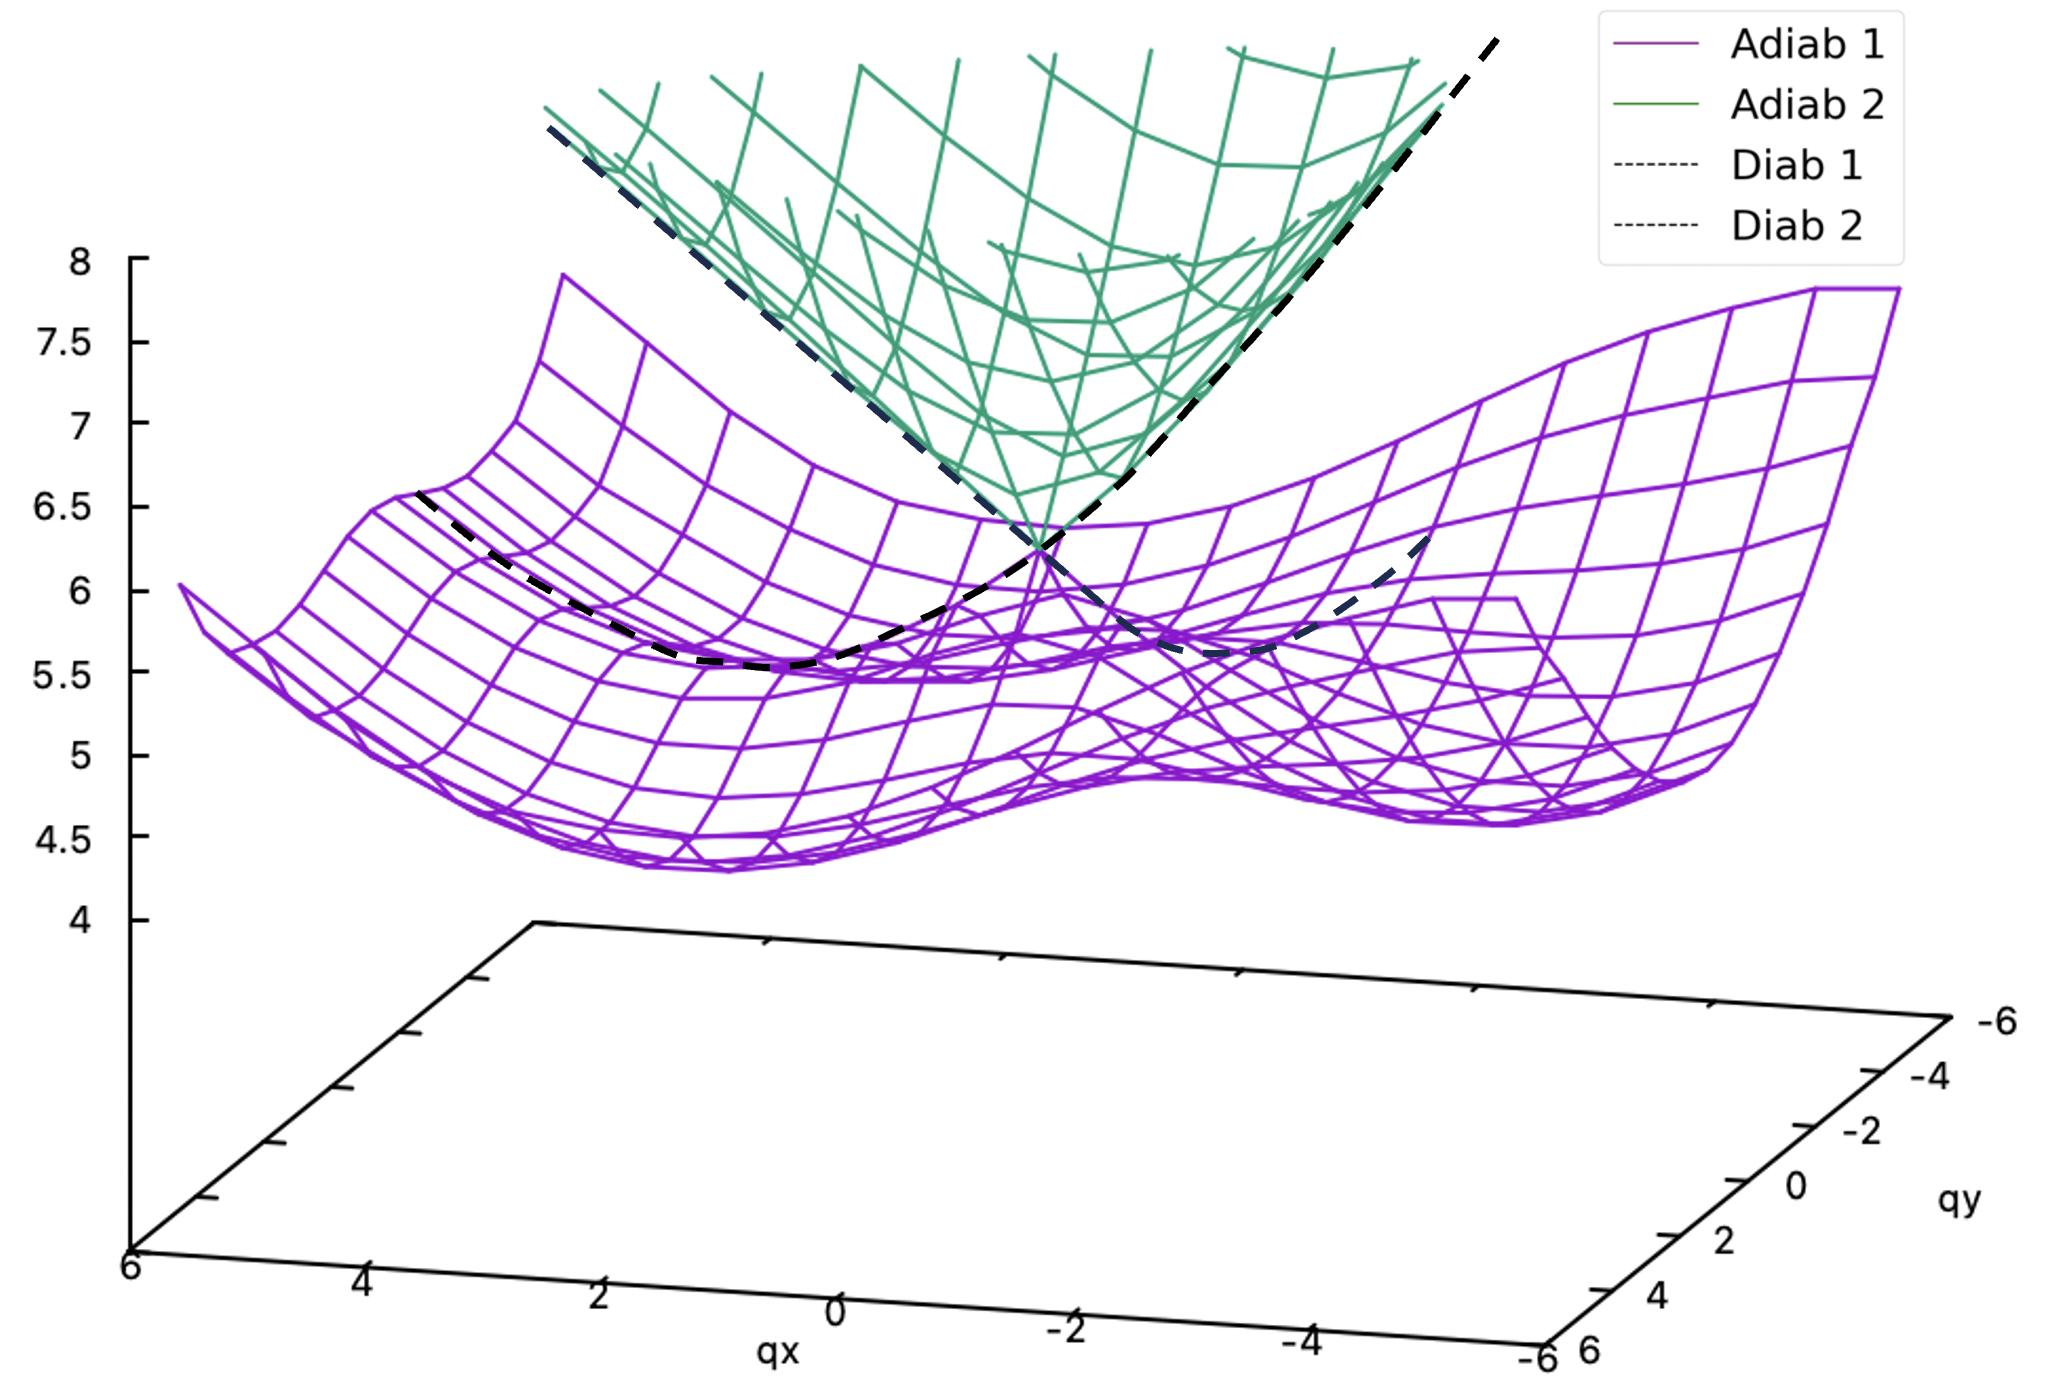
\includegraphics[width=0.75\linewidth,trim={0in 0in 0in 0in},clip]{images/updated_adiab_diab.png}
    \center
    \small{Fig 1. Stereotypical depiction of a conical intersection (CoIn) involving both adiabatic states (adiabats) and diabatic states (diabats) commonly seen in vibronic models. Source: Zeng.}
\end{figure}

The central goal in this project is to produce an accessible diabatization protocol that can supply MCTDH and VECC with vibronic model Hamiltonians suitable for a wide range of applications such as spin-orbit coupling (SOC) effects and spectroscopy. Since 2022 at the Nooijen and Zeng group, we have jointly endeavoured to pursue this goal.

% --------------------------------------------------------------------------------------------------
\section{Modern Vibronic Models - Timeline}
% --------------------------------------------------------------------------------------------------

% Rundown on the buildup towards the modern vibronic model protocol
The pioneering work of Cederbaum, Köppel, and Domcke gave rise to the original idea of vibronic models in their 1981 seminal paper~\cite{cederbaum1981multimode}. Determination of a vibronic model Hamiltonian that simultaneously coupled vibrational modes with an arbitrary set of electronic states was given in an \textit{ab initio} procedure. Their study proceeded to simulate spectroscopy and demonstrated the need for the inclusion of vibronic coupling effects to match with findings in experimental spectra. Neugebauer and Nooijen found this approach useful and further developed a diabatization scheme suitable for Time-dependent Density Functional Theory (TD-DFT) absorption spectrum~\cite{nooijen2003first,neugebauer2004vibronic}. Vibronic models were used at this point to model multiple potential energy surfaces in a limited region of configuration space, akin to a harmonic oscillator approximation applied to a single surface. Moreover, this established a formalized and standard method for extracting (from quantum chemistry calculations) vibronic model Hamiltonians in a routine fashion. Their scheme inspired Santoro and coworkers, who in recent years recasted Nooijen's scheme into a single-reference linear order Gaussian-MCTDH TD-DFT diabatization scheme purposed for studying the excited state dynamics of hexahelicene~\cite{yaghoubi2020ultrafast}. However, hexahelicene is merely an organic molecule. Ongoing frontier research by Domcke and Mondal aims to apply vibronic models for transition metal complex spectra, a notoriously difficult task due to the dilemma of low-lying degenerate electronic states. It is difficult to resolve the states and PES character for such systems. Therefore, a more ideal approach is to pivot towards a diabatization scheme that is multi-reference in nature, and can capture relativistic effects like spin-orbit coupling. \\

% This paragraph aims to justify Toby's contribution towards the field and basis of the GAMESS-SOC vibronic models
The existence of a diabatization protocol that includes spin-orbit coupling was first devised by Toby Zeng, an expert who specializes in vibronics and has massively contributed to the field of arbitrarily large Hamiltonian formalisms and Jahn-Teller (JT) interactions~\cite{zeng2017diabatization}. The foundation of the Zeng SOC protocol derives from previous work done by Atchity and Rudenberg on configurational uniformity. The protocol of interest specifically uses GAMESS-US package Generalized Multi-Configuration Quasidegenerate Perturbation Theory (GMC-QDPT) calculations. Diabatic states are directly calculated using Nakamura and Truhlar's version of configurational uniformity, whereby diabatic molecular orbitals (DMOs) are first prepared, and then computation of diabatic state functions follows. Calculations involved here are typed as multi-state multi-reference perturbation theory calculations in a given active space reference as generalized and implemented by Nakano. GMC-QDPT addresses the requisite Complete Active Space Self Consistent Field (CASSCF) component of the model. At this point, Zeng assembles all these pieces and opens up the possibility of adding spin orbit coupling terms to the model Hamiltonian. The basis of the vibronic models in this project will use the diabatic energies and couplings provided by this process. \\ 

Familiarity of transition metal vibronic models with SOC and spectroscopy is not recognized as new. To provide supplementary context, in 1999 Graham Worth of GAMESS and Nakano scrutinized the behaviour of $FeCO^+$ in a theoretical study. Domcke and Mondal have in particular investigated and discussed E x e Jahn-Teller and SOC effects in transition-metal fluorides, such as $CoF_3$ with a 17 orbital and 30 electron active space - CAS(30,17). Their analysis included generation of $D_{3h}$ trigonal planar symmetry vibronic model Hamiltonians and spectra. Zeng has previously applied the SOC protocol to pnictogen hydride cations with trigonal symmetry: $PH_3^+$, $AsH_3^+$, and $SbH_3^+$ for the purposes of investigating vibronic coupling and SOC characteristics. Zeng's protocol did not include spectroscopy components. The state of research so far builds up a case for which the project's diabatization protocol should be applied to: a large $D_{3h}$ iron-carbonyl complex with low-lying degenerate electronic states. The candidate molecule is $Fe(CO)_5$. If successful, the appealing challenge of $Fe(CO)_5$ should exhibit demonstrable JT, SOC, and photochemical effects as reported in the literature.

% An optimal and desirable system for exhibiting both JT and SOC effects is a large iron complex with low-lying degenerate electronic states and carbonyl ligand, due to carbonyls' known stabilizing effect on metals (Nooijen discussion referenece).
% Ultimately, the intersection of these previous explorations motivates a study converging on applying the Zeng protocol to a candidate $D_{3h}$ $Fe(CO)_5$ vibronic model system.


% --------------------------------------------------------------------------------------------------
%section{Scope: Vibronic Models Suitable for Transition Metal Complexes with Spin-orbit Coupling Effects}
\section{Project Scope: Pivot to Zeng Protocol and Limitations of Single-reference Linear Vibronic Models}
% --------------------------------------------------------------------------------------------------
To capitalize on all the work presented so far, I have created a novel automated diabatization code in Python to be incorporated into the Zeng SOC protocol. In my previous work, the Santoro protocol was used to generate vibronic models in Gaussian 16 for MCTDH testing. Naturally, they did not suffice for transition metal complexes. As shown in Fig 2, the vibronic models were found to not resolve any fine structure in metallic vibronic spectra, and for cases such as caffeine, the spectra was still inaccurate despite meticulous checking of the model. Santoro has likewise acknowledged the inaccuracies with using the linear protocol due to complications in finding correct parameters for calculations. The most pressing concern of using the Santoro protocol at the Nooijen lab was that the output vibronic model Hamiltonian (operator file) format was incompatible for VECC input.  

\begin{figure}[!ht]
    \center
    %\hspace*{-2cm}
    \includegraphics[width=1\columnwidth]{quad5.png}
    \small Fig 2. (a) Caffeine. Slightly matching peaks in the sub 240nm region observed, appears to need a linear red-shift for better agreement. (b) Titanium tetrachloride. The predictive accuracy here of a smooth single peak is recognized to be nowhere near reality, due to limitations of single reference TD-DFT methods applied to transition metal complexes.
\end{figure}

To improve on the capabilities of the vibronic models available for VECC, such limitations of the Santoro G-MCTDH method prompted for a pivoting towards the Zeng protocol. Prior to this project, only the top half path shown in Fig 3. (Santoro-MCTDH-Spectra) was explored. Here, VECC was also able to perform excited state simulations like MCTDH, however VECC's statistical mechanics ideally necessitate Zeng models for proper functionality. Therefore, to reiterate the declared task: we shall construct a composite approach where the Zeng protocol is first used to manufacture vibronic model Hamiltonians to be plugged in as input, and the latter half of non-adiabatic simulation shall be taken care of by VECC. A Zeng-VECC-Spectra pathway. Once the Zeng protocol can be successfully connected to both MCTDH and VECC, then it will allow for a variety of models and dataset to be used for practical comparison of the gold standard MCTDH method with the new VECC method.

\begin{figure}[!ht]
    \includegraphics[width=1\linewidth,trim={0in 0in 0in 0in},clip]{images/updated_scheme.png}
    \center
    \small{Fig 3. Original proposed research plan, the right half motivates the left half.}
\end{figure}

Formerly, the Zeng protocol diabatization was not automated. Each calculation in the series needed for full diabatization was handcrafted. In early 2023, Zeng completed the first step towards accomplishing the task: a prototype 'machine gun' bash code that automates diabatization. This version could effectively produce up to quadratic order Zeng non-SOC models, and was implemented to be extracted from GAMESS package calculations. Neil Raymond and I have iterated on the prototype and designed a full operating protocol. The code was first translated into Python, and then received a wide array of upgrades to ensure that it is SOC-compatible and readily plugged into MCTDH/VECC for spectroscopy.


\cleardoublepage


% --------------------------------------------------------------------------------------------------
%\subsection{Systems of Interest / Objectives (Most difficult system) } % maybe find different wording? 
%\subsection{Vibronic Models: Quadratic-order CASSCF GMCPT SOC Protocol} % Best case scenario
% --------------------------------------------------------------------------------------------------


% --------------------------------------------------------------------------------------------------

% --------------------------------------------------------------------------------------------------
\section{Outline of Thesis}
% --------------------------------------------------------------------------------------------------
In this thesis:
\begin{enumerate}
    \item The first chapter gives an overview of vibronics and the research project objectives.
    \item Fundamental quantum chemistry concepts and mathematics is presented.
    \item Full elucidation of Python code to automate the Zeng SOC protocol.
    \item Applications of the protocol to realistic transition metal systems and vibronic spectroscopy. 
    \item Conclusion and future outlook.
\end{enumerate}

\cleardoublepage

% --------------------------------------------------------------------------------------------------
% Rough notes from Neil 

% basically you just briefly introduce each chapter and its purpose
% see coco's and any body else's thesis'

% \section{Explanation of common terms} 
% maybe need to explain CASSCF GMCPT etc..? or you could explain in the section where you introduce them
% write later if needed
% Goal: introduce Vibronic (vib+elec) and diabatic models / diabatization protocols -> then give some specific example of why they're cool
% (why do we care (in general), and specific thing )
% \begin{enumerate}
%     \item BOA works for most systems, ignore specific math term
%     \item BUT, for interesting systems (Nonadaibatic) it is not sufficient and so we need new approaches
%     \item diabatic is one such approach, and it has various advantages. \\
% \end{enumerate}
% Application of diabatization methods to transition metal compound spectra. In a nutshell, this is very hard.

%     Fancy method, otherwise why not just DFT B3LYP 6-31G* @ everything ...


%     Analogy: we did not build the car, we merely are a driver, make sure we diligently perform routine maintenance on it, know what engine is and how to fill gas, etc. 

%     We do not construct a car from the ground up, not feasible... monumental task


% \begin{enumerate}
%     \item provide background for the general version/style (Open-shell transition metal complex) of Fe(CO)5 
%     (you could mention / use the D3h systems you trained on as general examples... you don't have to, just if its useful to draw on that experience)
    
%     \item introduce the specifics of Fe(CO)5 

%     \item  Describe Jahn-Teller effect and spin-orbit coupling effect in transition metal chemistry.

%     1,2,3,4,5,6,7,8
%     somewhere in intro you should explain what CASSCF is.
%     go look at CHEM gaussian course notes from jake + textbook or two (marcel/fred?/toby might have a textbook to recommmend)
    
    
%     \item talk about challenges and other stuff?


% \end{enumerate}

% --------------------------------------------------------------------------------------------------


% --------------------------------------------------------------------------------------------------
% --------------------------------------------------------------------------------------------------
\chapter{Theoretical Overview and Methodology} % Methods and Context
% --------------------------------------------------------------------------------------------------


% --------------------------------------------------------------------------------------------------
\section{Electronic structure theory}
% --------------------------------------------------------------------------------------------------
In an ideal world, the Schrödinger equation would be readily solved by computers and the exact solution for energy would be known. 
    
% --------------------------------------------------------------------------------------------------
%%%%% TAKEN FROM 494, JUST FOR REFERENCE
    Let the full molecular Schrödinger's Equation be defined as: 
\begin{equation}\label{eq:schrodinger}
    \begin{split}
        \hat{H}(\Vec{R}) \Psi_{n}(\Vec{r};\Vec{R}) = E_n \Psi_{n}(\Vec{r};\Vec{R})
    \end{split}
\end{equation}
%
The full molecular Hamiltonian:
\begin{equation}%\label{eq:eqnlabel}
    \begin{split}
        \hat{H} = -\sum_{\alpha}^{M} \frac{1}{2M_{\alpha}} \nabla_{\alpha} \cdot \nabla_{\alpha}
         -\sum_{i}^{N} \frac{1}{2m_{e}} \nabla_{i} \cdot \nabla_{i}
         + \sum_{i,j>i}^{N} \frac{1}{r_{ij}} + \sum_{i, \alpha}^{N,M} \frac{-Z_{A}}{r_{i\alpha}}
         + \sum_{\alpha, \beta \neq \alpha}^{M} \frac{Z_{A}Z_{B}}{R_{\alpha \beta}}
    \end{split}
\end{equation}
%
Which can concisely be represented by kinetic and potential energy operators $\hat{T}$ and $\hat{V}$:
\begin{equation}%\label{eq:eqnlabel}
    \begin{split}
        \hat{H} = \hat{T}_{N} + \hat{T}_{e} + \hat{V}_{ee} + \hat{V}_{Ne} + \hat{V}_{NN}
    \end{split}
\end{equation}
%
Note the subscripts $e, N$ are for electronic and nuclear correspondingly.
\begin{equation}%\label{eq:eqnlabel}
    \begin{split}
        \hat{H}_{} = \hat{T}_{N} + \hat{H}_{elec} 
    \end{split}
\end{equation}
%
\begin{equation}%\label{eq:eqnlabel}
    \begin{split}
        \hat{H}_{elec} = \hat{T}_{e} + \hat{V}_{ee} + \hat{V}_{Ne} + \hat{V}_{NN}
    \end{split}
\end{equation}
%$\hat{H}_{elec}$ critically does not include the nuclear-kinetic term $\hat{T}_{N}$. 
\\ Let the wavefunction, $\Psi$, be the sum over the electronic eigenstates $\phi_{\lambda} (\Vec{r};\Vec{R})$ and nuclear eigenstates $\chi_{\lambda} (\Vec{R})$:
\begin{equation}%\label{eq:eqnlabel}
    \begin{split}
        \Psi (\Vec{r};\Vec{R}) = \sum_{\lambda} \phi_{\lambda} (\Vec{r};\Vec{R}) \chi_{\lambda} (\Vec{R})
    \end{split}
\end{equation}
Here, $\Vec{r}$ indicates electron coordinates, and $\Vec{R}$ refers to nuclear configuration. The subscripts $\lambda$ and $\mu$ denote electronic states. To describe a parametric dependence of $\Vec{r}$ on $\Vec{R}$, $(\Vec{r};\Vec{R})$ is used. Signifying that although an explicit dependence on $\Vec{R}$ is not present in the function, $\Vec{r}$ values are predicated at a single $\Vec{R}$ parameter~\cite{szabo2012modern}. Therefore, if $\Vec{R}$ changes, so does $\phi_{\lambda}(\Vec{r};\Vec{R})$. \\
Proceed with full expansion of Hamiltonian acting on the wavefunction:
\begin{subequations}\begin{align}%\label{eq:eqnlabel}
    &\hat{H} (\Vec{R}) \Psi (\Vec{r};\Vec{R})\nonumber
\\  
    &=
    \left[ 
        - \sum_{\alpha} \frac{1}{2M_{\alpha}} \Vec{\nabla_{\alpha}} \cdot \Vec{\nabla_{\alpha}}   + \hat{H}_{elec} 
    \right]
    \left[ 
        \sum_{\lambda} \phi_{\lambda} (\Vec{r};\Vec{R}) \chi_{\lambda} \Vec{(R)}
    \right]
\\
    \begin{split}
        &=
        \Big( - \sum_{\alpha} \frac{1}{2M_{\alpha}} ~\Big) \sum_{\lambda} 
        [ 
            \chi_{\lambda} \Vec{(R)} \Vec{\nabla^{2}_{\alpha}} \phi_{\lambda} (\Vec{r};\Vec{R})
            + \Vec{\nabla_{\alpha}} \phi_{\lambda} (\Vec{r};\Vec{R}) \Vec{\nabla_{\alpha}} \chi_{\lambda}
        \\  &\qquad\qquad
            + \phi_{\lambda} (\Vec{r};\Vec{R}) \Vec{\nabla^{2}_{\alpha}} \chi_{\lambda} \Vec{(R)}
            + \Vec{\nabla_{\alpha}} \chi_{\lambda} \Vec{\nabla_{\alpha}} \phi_{\lambda} (\Vec{r};\Vec{R})
            + E_{\lambda}(\Vec{R}) \phi_{\lambda}(\Vec{r};\Vec{R}) \chi_{\lambda} \Vec{(R)} 
        ]
    \end{split} 
\\  
    \begin{split}
        &=
        \Big( - \sum_{\alpha} \frac{1}{2M_{\alpha}} ~\Big) \sum_{\lambda} 
        [ 
            \chi_{\lambda} \Vec{(R)} \Vec{\nabla^{2}_{\alpha}} \phi_{\lambda} (\Vec{r};\Vec{R}) 
        \\  &\qquad\qquad
            + \phi_{\lambda} (\Vec{r};\Vec{R}) \Vec{\nabla^{2}_{\alpha}} \chi_{\lambda} \Vec{(R)} 
            + 2\Vec{\nabla_{\alpha}} \phi_{\lambda} (\Vec{r};\Vec{R}) \Vec{\nabla_{\alpha}} \chi_{\lambda} 
            + E_{\lambda}(\Vec{R}) \phi_{\lambda}(\Vec{r};\Vec{R}) \chi_{\lambda} \Vec{(R)} 
        ]
    \end{split}
\end{align}\end{subequations}
%
Integrating against $\phi_{\mu} (\Vec{r},\Vec{R})$ over all electronic coordinates, $\Vec{r}$, and asserting that these states are orthonormal at a single fixed $\Vec{R}$, produces a sum of four terms:
% a possible alternative layout to your current ABCD thing
 \begin{align} 
   \tag{\textbf{A}}\label{eq:A2}
     &= \sum_{\lambda} \int \phi_{\mu}^{*} (\Vec{r};\Vec{R}) \sum_{\alpha} - \frac{1}{2M_{\alpha}} \Vec{\nabla_{\alpha}^{2}} \phi_{\lambda} (\Vec{r};\Vec{R})~dr \chi_{\lambda} \Vec{(R)}
     %
     %
 \\  \tag{\textbf{B}}\label{eq:B2}
     %
     &\qquad+ \sum_{\lambda} \sum_{\alpha} \delta_{\lambda \mu} \frac{-1}{2M_{\alpha}} \Vec{\nabla_{\alpha}^{2}}  \chi_{\lambda} \Vec{(R)}
     %
     %
     \\  \tag{\textbf{C}}\label{eq:C2}
     %
     &\qquad+ \sum_{\lambda} \sum_{\alpha} \int \phi_{\mu}^{*} (\Vec{r};\Vec{R}) \Vec{\nabla_{\alpha}} \phi_{\lambda} (\Vec{r};\Vec{R}) dr \cdot - \frac{1}{2M_{\alpha}} \Vec{\nabla_{\alpha}} \chi_{\lambda} \Vec{(R)}
     %
     %
     \\  \tag{\textbf{D}}\label{eq:D2}
     %
     &\qquad+ \sum_{\lambda} \delta_{\lambda \mu} E_{\lambda} (\Vec{R}) \chi_{\lambda} \Vec{(R)}
     \\ &= \sum_{\lambda} E_{\lambda} \Vec{(R)}  \delta_{\lambda \mu} \chi_{\lambda} \Vec{(R)}
 \end{align}

The BOA facilitates setting the expansion in terms of a single electronic state, hence $\lambda = \mu$. Terms \textbf{A} and \textbf{C} in the BOA are also ignored. The \textbf{A} term represents a diagonal Born-Oppenheimer correction to potential, useful in specialized instances--as in accounting for different $M_{\alpha}$ (e.g. isotopes)~\cite{nooijennotes}. It is typically proximate enough to zero for it to be neglected. Likewise, \textbf{C} is zero for real normalized wavefunctions. \textbf{C} is referred to as the off-diagonal non-adiabatic coupling (NAC) terms. In other words, only \textbf{B} and \textbf{D} terms remain because terms with the presence of $\int dr \Vec{\nabla_{\alpha}} \phi_{\lambda} (\Vec{r};\Vec{R})$ are effectively zero if there exists little change in $\phi_{\lambda}$ with respect to $\Vec{R}$, thus implying no coupling between electronic wavefunctions and nuclear configuration~\cite{nooijennotes}. 
\\
As for a small example, so far the BOA shows:
\begin{equation}%\label{eq:eqnlabel}
    \begin{split}
        \begin{bmatrix}
            \hat{T}_N + E_{1}(\Vec{R}) + A_{1}(\Vec{R}) & N.A.C.\\
            N.A.C.& \hat{T}_N + E_{2}{(\Vec{R}) + A_{2}(\Vec{R})}
        \end{bmatrix}
    \end{split}
\end{equation}

Ultimately, the Schrödinger equation with the BOA applied appears as:
\begin{equation}\label{eq:10}
    \begin{split} 
            \left[ \hat{T}_N + E_{\lambda} \Vec{(R)} \right] \Psi_{\lambda, n} \Vec{(R)} = E_{n} \Psi_{\lambda. n} \Vec{(R)}
    \end{split}
\end{equation}
Where label $n$ is for rotational-vibrational levels and recalling $\lambda$ is for electronic states. Attention to the term $E_{\lambda}(\Vec{R})$, which is a function of nuclear configuration. % Unlike the case for the full molecular Schrödinger equation, where energy is a constant (which is not a functional of coordinates), 
$E_{\lambda}(\Vec{R})$ is defined to be a single point sufficiently able to define a potential energy surface (PES), $E_{\lambda}(\{ \Vec{R} \})$. Now the electronic wavefunction $\phi_{\lambda} (\Vec{r};\Vec{R})$, wavefunction $\chi_{n} (\Vec{R})$ (detailing nuclear motion), and potential energy surface $E_{\lambda} \Vec{(R)}$ in \Cref{eq:10} can be solved for  at a single electronic state $\lambda$ with any given fixed-geometry $\Vec{R}$. In practice of using BOA concepts, \Cref{fig:fig1} demonstrates how the electronic ground state PES can be theoretically constructed. Understanding surfaces in this fashion gives rise to adiabatic states or true Born-Oppenheimer surfaces~\cite{villanueva2020spectroscopic}. 
\\
\begin{figure}[!h]
    \center
    \includegraphics[width=0.9\linewidth]{images/boa_gs.png}
    \caption[Depiction of a BOA Electronic Ground State Surface ]{\label{fig:fig1} A single electronic ground state surface within the BOA leads to sampling and subsequently calculating points at fixed nuclear configurations $(\Vec{R}_a, \cdots, \Vec{R}_b, \cdots)$.}
\end{figure}

\newpage
% -------------------------------------------------------
\subsection{Adiabatic and Diabatic Basis Connection}
% -------------------------------------------------------
%Focus is now directed towards excited states. 
Earlier discussions on the importance of non-adiabatic dynamics to vibronic models and spectra can now deepen. Although the BOA was highlighted to reduce calculation complexity (i.e. avoiding evaluation of integral terms), it fails when the NACs are relevant--\Cref{fig:fig2}(a), occurring mainly in two situations:
\begin{enumerate}[label=\roman*.]
    \item The adiabatic state character changes rapidly as a function of geometry.
    \item Degenerate electronic states, separations on the order of vibrational energy level values.
\end{enumerate}

When these conditions exist, Yarkony has described how conical intersections and avoided crossings between separate single excited states develop, and in order to simulate spectra successfully, the model needs to account for neglected terms and be governed by multiple PES to describe nuclear motion~\cite{yarkony2001conical}. %The BOA simply cannot be applied anymore. This indicates a departure from the adiabatic (BOA) basis, namely to a non-adiabatic process that requires invoking diabatic states. %Vibronic coupling theory can assist in simulating the non-adiabatic system.
\\ 
Recall, term \textbf{C} contains an integral, which is inversely proportional to energy separation:
\begin{equation}\label{eq:inverseproportional}
    \begin{split}
            \int \phi_{\mu}^{*} (\Vec{r};\Vec{R}) \Vec{\nabla_{\alpha}} \phi_{\lambda} (\Vec{r};\Vec{R})~dr 
            \propto \frac{1}{E_{\mu} - E_{\lambda}}
    \end{split}
\end{equation}

Ultimately, the Schrödinger equation with the BOA applied appears as:
\begin{equation}\label{eq:10a}
    \begin{split} 
            \left[ \hat{T}_N + E_{\lambda} \Vec{(R)} \right] \Psi_{\lambda, n} \Vec{(R)} = E_{n} \Psi_{\lambda. n} \Vec{(R)}
    \end{split}
\end{equation}

\begin{equation}\label{eq:atodmatrix}
    \begin{split}
        \begin{bmatrix}
            \hat{T}_N + E_{1}(\Vec{R}) + A_{1}(\Vec{R}) & N.A.C.\\
            N.A.C.& \hat{T}_N + E_{2}{(\Vec{R}) + A_{2}(\Vec{R})}
        \end{bmatrix}
        \Rightarrow
        \begin{bmatrix}
            \hat{T}_{N} + E_{11}(\Vec{R}) & E_{12}(\Vec{R}) \\ 
            E_{21}(\Vec{R}) & \hat{T}_{N} + E_{22}{(\Vec{R})}
        \end{bmatrix}
    \end{split}
\end{equation}
%
Obtaining this matrix of diabatic form, it can be utilized to describe potentials and a coupled set of vibrational wavefunctions $\chi_a(\Vec{R})$:
\begin{equation} 
    \begin{split}
        \begin{pmatrix}
            \hat{T}_{N} + E_{11}(\Vec{R}) & E_{12}(\Vec{R}) \\ 
            E_{21}(\Vec{R}) & \hat{T}_{N} + E_{22}{(\Vec{R})}
        \end{pmatrix}
        %
        \begin{pmatrix}
            \chi_{1}(\Vec{R}) \\ 
            \chi_{2}(\Vec{R})
        \end{pmatrix} 
        = E
        %
        \begin{pmatrix}
            \chi_{1}(\Vec{R}) \\ 
            \chi_{2}(\Vec{R})
        \end{pmatrix} 
    \end{split}
\end{equation}

\begin{equation}\label{eq:diabaticstates}
    \begin{split}
            \Psi_{a}(\Vec{r};\Vec{R}) = \sum_{\lambda} U_{\lambda a} (\Vec{R}) \phi_{\lambda} (\Vec{r};\Vec{R})
    \end{split}
\end{equation}

\begin{equation}\label{eq:overlapmatrix}
    \begin{split}
            S_{\lambda \mu}(\Vec{R}) = \int \phi_{\mu}^{*} (\Vec{r};\Vec{R}_{q_0}) \phi_{\lambda} (\Vec{r};\Vec{R}_{q_0 \pm dq_{i}})
    \end{split}
\end{equation}

\begin{equation}%\label{eq:eqnlabel}
    \begin{split}
            \sum_{\lambda} \int \phi_{\mu}^{*} (\Vec{r};\Vec{R})
            %\Vec{\nabla_{\alpha}}
            \hat{H}_{elec} \Psi_{a}(\Vec{r};\Vec{R}) \phi_{\lambda} (\Vec{r};\Vec{R}) dr
            %\cdot - \frac{1}{2M_{\alpha}} \Vec{\nabla_{\alpha}}
            \chi_{\lambda} \Vec{(R)}
            = \sum_{\lambda} E_{\mu \lambda} \chi_{\lambda} \Vec{(R)}
    \end{split}
\end{equation}

\begin{equation} \label{eq:17}
    \begin{split}
            E_{\mu \lambda} (q) = E_{\mu \lambda} (0) + \sum_{i}^{M} E_{\mu \lambda}^{i}q_i + \frac{1}{2} 
            \sum_{i>j}^{M} E_{\mu \lambda}^{ij}q_{i}q_{j} + \cdots
    \end{split}
\end{equation}

\begin{equation} \label{eq:18}
    \begin{split}
            E_{\mu \lambda}^{i} = \frac{E_{\mu \lambda} (\Vec{R}_{q_0} + dq_{i}) - E_{\mu \lambda} (\Vec{R}_{q_0} - dq_{i})}{2dq_{i}}
    \end{split}
\end{equation}
\cleardoublepage


% --------------------------------------------------------------------------------------------------
\section{Non-adiabatic Chemistry Applications}
%%%%%%%%%%% REWRITE THIS %%%%%%%%%%%%
% --------------------------------------------------------------------------------------------------
Emerging research on vibronic models has led to many fascinating discoveries.  Through examination of the couplings between electronic states and nuclear motion, the interesting mechanics behind vision in the eye, which is a sophisticated biological system, can be properly understood. There has been realization that photo-isomerization of retinal can be attributed to involving radiation-less decay pathways. Such pathways are rather puzzling if not for a non-adiabatic picture. This picture can demonstrate how after capturing a photon, retinal's excited state can transition and cross into its ground state without fluorescence~\cite{schnedermann2016vibronic}. Non-adiabatic dynamics occur when electronic states' separations are small, and can lead to developing these interesting concepts of conical intersections regions, inter-system crossings, and multi-character electronic states. Non-adiabatic dynamics and photochemical processes are at the heart of what vibronic models can explain.

% --------------------------------------------------------------------------------------------------
\section{Spectroscopy}
%%%%%%%%%%% TO BE WRITTTEN %%%%%%%%%%%%
Traditional Franck-Condon approach to simulate spectroscopy.

\cleardoublepage


\subsection{MCSCF, CASSCF, GMC-QDPT}
        %%% TAKEN FROM PROPOSAL %%%%
        \subsubsection{Diabatic Molecular Orbitals}
        Configurational uniformity's implementation in GAMESS is a concept devised by Nakamura and Truhlar to manufacture diabats from adiabats. In their framework, which expands on previous work by Atchity and Rudenberg, diabatization-adapted molecular orbitals (DMOs) are obtained and then subsequent DSFs (diabatic state functiosn) are constructed. The idea is to optimize for uniformity in electronic configurations that originate from DMOs. Model space.
    

        \subsubsection{GMC-QDPT}
        Haruyuki Nakano and coworkers have devised the Generalized Multiconfiguration - Quasi Degenerate Perturbation Theory (GMC-QDPT) scheme. GMC-QDPT itself is classified as a composite method that aims to recover both static and dynamical correlation. The 'generalized' label refers to zero-restrictions in variational space. This means beyond CASSCF and RASSCF, so general MCSCF wavefunctions are applicable for submission as input. The QDPT latter half indicates a subsequent multireference calculation that proceeds. In short, it is intended for multistate calculations, and optimal for heavy/relativistic calculation purposes. Interestingly, when benchmarked with CAS-QDPT, there is only a 0.1 eV and 1 kcal/mol $\Delta$. Nakano has prepared an excellent student reference guide for performing GAMESS GMCPT and GMC-QDPT calculations: {https://ccl.scc.kyushu-u.ac.jp/\~nakano/gmcpt.html}. An important consideration is that FCI is often intractable due to the computational cost growing factorially in terms of reference space determinants, so this efficient scheme is more feasible instead.

        \cleardoublepage

        \subsubsection{Active Space Design}
        Designing the active space is a pedantic problem.
        
        Cool paper: \url{https://arxiv.org/pdf/2111.15587#:~:text=ORMAS%20is%20a%20construction%20of,and%20minimum%20number%20of%20electrons.}


    %--------------------------------------------------------------------------------------------------------


    
%--------------------------------------------------------------------------------------------------------
\section{Jahn-Teller and Relativistic Effects}

%--------------------------------------------------------------------------------------------------------
    \subsection{Group Theory and Symmetry}

    \subsection{Spin Orbit Coupling (SOC)}
%--------------------------------------------------------------------------------------------------------


%--------------------------------------------------------------------------------------------------------
\section{Calculation of Spectra}
%--------------------------------------------------------------------------------------------------------
    %--------------------------------------------------------------------------------------------------------
    \subsection{Traditional Franck-Condon}
    
    %--------------------------------------------------------------------------------------------------------
    \subsection{Time-correlation functions}
    
    %--------------------------------------------------------------------------------------------------------
    \subsection{MCTDH}
    Consultation with Dieter Meyer of MCTDH
    
    %--------------------------------------------------------------------------------------------------------
    \subsection{VECC}
    VECC Paper: https://arxiv.org/pdf/2312.14164.pdf
    Our model comparisons have the following assumptions: although we can submit more information to MCTDH than VECC (e.g. off-diagonal coupling of state energies and excited state-to-state transition dipole moments), our comparisons are limited to whatever VECC accepts. Therefore, the difficulty arises from finding a hybrid format compatible to both dynamics-simulation-schemes that can capture the model. A technical challenge, mainly.

    Focusing on VECC, it is potentially advantageous due to its generation of results in a theoretical O(n2) time scaling, where
n is the number of normal modes. In comparison, the modern multi-layer MCTDH approach is com-
putationally uneconomical with its exponential scaling and requires extensive user input to dictate
efficient calculation. Despite VECC being less systematic, it has the critical advantage of demanding
very few user choices; limited to simple on/off switches. VECC’s present implementation requires
construction of vibronic model Hamiltonians to be plugged in as input, which is likewise an expensive
and tedious task.

    \subsection{Thermal Effects: Thermal Field Vibrational Electronic CC (TF-VECC)}


\section{Computational Hardware and Software}

\subsection{GAMESS-US}
GAMESS is an ab initio quantum chemistry package. The general pipeline of how calculations are run: HF/DFT/GVB/MCSCF $\Rightarrow$ CI/MP2/CC (these are correlation corrections) $\Rightarrow$ SOC/DK (these are relativistic effect corrections). One interesting thing about GAMESS is that recently there is possibility for GPU-acceleration. 

Fancy method, otherwise why not just DFT B3LYP 6-31G* @ everything ...
\newpage
%--------------------------------------------------------------------------------------------------------
    
    \subsection{nlogn, ComputeCanada (Computational Resources)}
    On nlogn, the available compute is as follows:
    cpu[005-006] intel,westmere, X5670 12 48000 io003 intel,ivybridge,E5-2 16 128000 io[001-002] intel,westmere,X5670 12 48000 \\

    On ComputeCanada Graham cluster, the available compute per node is 32 CPUs with 125GB of memory. \\

    The GAMESS memory requirements for parallelized calculations is as follows: ((mwords * p + memddi)*8) / 1024 = TOTAL NUMBER OF GB. Where p is the number of processors, mwords is the amount of memory (in Words) for each processor, memddi is the distributed memory for optimization runs, and 8/1024 to account for the conversion of words to gigabytes. Therefore, on nlogn, the max amount of compute per run would be 16 CPUs at 4 gigabytes. For reference, see https://docs.alliancecan.ca/wiki/GAMESS-US. \\

    To compile Zeng's GMC-QDPT compatible GAMESS version on ComputeCanada clusters, it is complicated. First, the \textit{gmcpt.src} module must be obtained from Zeng. The next step is to \textit{module load intel/2023.2.1} and run \textit{./config} in GMS' source directory; this will prompt a set of questions in which the answers are as follows: linux64, enter, enter, enter, ifort, 10, none. After you msut enter the ddi/ directory and run ./compddi and move the ddikick executable one directory above. Finally, you must run ./lked to link GAMESS to your path.
\newpage


% ------------------------------------------------------------------------------------
% ------------------------------------------------------------------------------------
\chapter{Diabatization and Spectroscopy Protocol in Practice} % your contribution?
% ------------------------------------------------------------------------------------
An explanation of the current vibronic model generation process will be presented. The basic flow is: 1) CASSCF 2) Diabatization 3) Spectroscopy. Human custom input is needed to setup the first four steps in the CASSCF component, which revolves around dictating parameters such as active space and reference geometry; step five is where the Python automated code enters to fulfill diabatization. After the diabatization calculations are complete, vibronic Hamiltonians can be harvested, wavepackets propagated, and spectra generated.
% ------------------------------------------------------------------------------------
\section{CASSCF Pipeline} 
% ------------------------------------------------------------------------------------
% the point being that you explain step-by-step how the protocol works.
% maybe one section in chapter three should be a full example of calculating water or D3h or some such model with SOC? showing the sections of the text files that you have to strip out, and the values etc.
% ------------------------------------------------------------------------------------
The approach taken here is a slightly modified version as seen in %sed in Aranda and Santoro’s work [19]. 
Zeng's work. \ce{RhF3} molecule will be used as an example.
\newpage

The CASSCF stage has, broadly, five phases:

\begin{figure}[!ht]
    \makebox[\textwidth][c]{%
        \includegraphics[width=1.25\linewidth,trim={0in 0in 0in 0in},clip]{images/nice_computational_protocol_Toby.pdf}
    }
    \caption{\small{GMC-QDPT CASSCF vibronic coupling model scheme formulated by Zeng.}}
\end{figure}

\begin{enumerate}[nosep]
  \item \Cref{sec:cx-diabatization_in_practice_1}: Geometry optimization and frequency calculations.
  \item \Cref{sec:cx-diabatization_in_practice_2}: Calculating adiabatic states at reference geometry using single-point GMCPT calculation. Active space selection is required.
  \item \Cref{sec:cx-diabatization_in_practice_3}: Use semi-canonical orbitals to obtain diabatic molecular orbitals (DMO). 
  \item \Cref{sec:cx-diabatization_in_practice_4}: Perform reference determinants selection and select states to compose Adiabat-to-Diabat matrix. Diabatization template is obtained.
  \item \Cref{sec:cx-diabatization_in_practice_5}: Machine gun diabatization and evaluating the electronic integrals (via submitting an array of GAMESS calculations) at distorted geometries. Collating numerical results and return .op/.json files.
\end{enumerate}


The first four steps are completely carried out in GAMESS. There exists supplementary Python scripts that can aid in each step. In particular, \textit{combined\_toolkit.py} offers a collected package of useful scripts that can extract or calculate critical information needed at each step. \textit{subgam.diab} is a GAMESS job submission script that can take an input file and send it to the queue.

\cleardoublepage

%see SECTION 2.4 in Neil's thesis

% ------------------------------------------------------------------------------------
\subsection{Step 1: Geometry optimization + frequency (Hessian)\label{sec:cx-diabatization_in_practice_1}}

Following standard practice for GAMESS users, input geometry coordinates are first set using the wxMacMolPlt GUI builder tool. Typically the \textit{$\$data$} group appears as follows, and GAMESS will duplicate the single fluorine atom given by the appropriate $D_3h$ geometry.
\\
\begin{lstlisting}[language=Fortran, caption=Example RhF3 Input Geometry]
 $data
 DNH 3

 Rh    45.0    0.0  0.0  0.0
 F      9.0    2.07 0.0  0.0
 $end
\end{lstlisting}

%--------------------------------------------------------------------------------------------------------
    
\begin{table}[h!]
    \centering
    \caption[Step 1 Information]{\label{table:one} Step 1 information.}
    \begin{tabular}{ c|c }
        \toprule
        Input & Output 
    \\  \midrule
    %
    \\
    \verb|subgam.diab| &
    \\
    \verb|RhF3_SPK_mp2_rohf_D3h_mult5_diis_gh.inp| & \verb|*_gh.out| 
    \\
    \\
        \bottomrule
    \end{tabular}
\end{table}

\cleardoublepage
% --------------------------------------------------------------------------------------------------
% ------------------------------------------------------------------------------------
\subsection{Step 2:\label{sec:cx-diabatization_in_practice_2}}
% optional sections 
This is the critical CASSCF active space setup step. To elucidate the active space without prior intuition is a challenging task. Many iterations on assessing the orbitals and adjusting the dimensions of the active space were needed. This human in the loop
\subsubsection{Talk about GMCPT characteristics}

%--------------------------------------------------------------------------------------------------------
    
\begin{table}[h!]
    \center
    \caption[Step 1 Information]{\label{table:two} Step 2 information.}
    \begin{tabular}{ c||c|c c }
        \toprule
        Command Line & Input & Output 
    \\  \midrule\midrule
    %
        \verb|python3 step0.py| & &
    \\  & &
    \\  Manual execution: & \verb|molecule_optfreq.com| & \verb|molecule_optfreq.log| 
    \\  \verb|python3 step1.py| &  & \verb|master_values.json|
    \\  & &
    \\  Automated execution: & &
    \\  \verb|python3 automate_scripts.py -1|  & &
    \\
        \bottomrule
        \end{tabular}
\end{table}
% --------------------------------------------------------------------------------------------------

% ------------------------------------------------------------------------------------
\subsection{Step 3: DMO Calculation\label{sec:cx-diabatization_in_practice_3}}
mx
\subsubsection{Discuss semi canonical orbitals to DMO}

%--------------------------------------------------------------------------------------------------------
    
\begin{table}[h!]
    \center
    \caption[Step 1 Information]{\label{table:one} Step 1 information.}
    \begin{tabular}{ c||c|c c }
        \toprule
        Command Line & Input & Output 
    \\  \midrule\midrule
    %
        \verb|python3 step0.py| & &
    \\  & &
    \\  Manual execution: & \verb|molecule_optfreq.com| & \verb|molecule_optfreq.log| 
    \\  \verb|python3 step1.py| &  & \verb|master_values.json|
    \\  & &
    \\  Automated execution: & &
    \\  \verb|python3 automate_scripts.py -1|  & &
    \\
        \bottomrule
        \end{tabular}
\end{table}
% --------------------------------------------------------------------------------------------------

% ------------------------------------------------------------------------------------
\subsection{Step 4:\label{sec:cx-diabatization_in_practice_4}}

\begin{lstlisting}[language=Fortran, caption=Example RhF3 Input Geometry]


 !Step 2: Sinple point gmcpt calculation for RhF3 model.
 $system kdiag=3 mwords=200 memddi=3000 parall=.t. $end
 $contrl runtyp=energy ispher=1 relwfn=LUT-IOTC $end
 $contrl icut=9 itol=20 inttyp=rysquad qmttol=1.0d-05 nosym=1 $end
 $scf    npunch=2 conv=1.0d-06 dirscf=.t. diis=.t. soscf=.f. ethrsh=10.0 $end
 $contrl scftyp=mcscf  mult=5 maxit=200 icharg=0 mplevl=2 $end
 $guess  guess=moread norb=168 purify=.t. $end
 $basis  gbasis=SPKrTZP $end
 $mcscf  cistep=gmcci fullnr=.t. finci=mos
         acurcy=1.d-6 maxit=200 $end
 $trans  dirtrf=.t. $end
 $mrmp   mrpt=gmcpt rdvecs=.f. $end
 $gmcpt  nmofzc=21 nmodoc=12 nmoact=5 nelact=6 stsym(1)=A nsolut=100
         reftyp=ormas nspace=1 mstart(1)=34 mine(1)=6 maxe(1)=6
         kstate(1)=1,1,1,1,1,1,1,1,1,1,1,1,1,1,1
         wstate(1)=1,1,1,1,1,1,1,1,1,1,1,1,1,1,1
         iwgt=0 thrwgt=-1.0 krot=.f. kszdoe=.f. knospn=.t.
         thrde=-1.0 edshft=0.02 $end
 $statpt hssend=.t. $end
 $transt $end
 -data
 RhF3 3 state calculation
 C1
 RH         45.0   0.0000000000  -0.0000000000   0.0000000000
 F           9.0  -0.9363534495   1.6218117484   0.0000000000
 F           9.0  -0.9363534495  -1.6218117484   0.0000000000
 F           9.0   1.8727068990   0.0000000000   0.0000000000
 $end
 \end{lstlisting}
% \subsubsection{Details about differences between MCTDH and VECC? maybe?}

\subsection{Step 5: temp.inp\label{sec:cx-diabatization_in_practice_5}}
\subsubsection{Details about making temp.inp}

% optional section to explain assorted edge cases 
\section{Comments on further details of protocol (and other random edge cases)} 


% ------------------------------------------------------------------------------------
%\section{CASSCF}
% ------------------------------------------------------------------------------------
    
%======================================================================
\section{Automated Machine Gun Diabatization Code: \\ \textit{'dist\_allmodes\_pm.py'}\label{sec:s1}}
%======================================================================
Majority of the code implementation was done in collaboration with Neil Raymond. Code to perform the described procedure is publicly available on GitHub: \url{https://github.com/bjb2chen/VEmodel}. Additionally, inside the repository are accompanying videos with commentary running through the full fledged protocol from input geometry to spectra. 

\subsection{Step 1: Collect Geom opt + Freq results\label{dstep1}}
\subsubsection{Details about text extraction and arrays}


\textit{combined\_toolkit.py} is simply a collection of 8 utilities that are useful in preparing the diabatization template:

\subsection{Step 2: Submit diabatization calculations Displacements\label{dstep1}}

\subsubsection{Special details about +1/+2/+3/+4}
\subsubsection{Special details about selecting certain modes to have +8 etc}



\begin{lstlisting}[language=Python, caption=Precomputing linear displacements]

# -----------------------------------------------------------------------
# NEIL MAGIC CODE (^o^)
displacements = {
"+1": reference[:, NEW] + 1.0 * R_array[NEW, :] * mode_array[:, :],
"-1": reference[:, NEW] - 1.0 * R_array[NEW, :] * mode_array[:, :],
"+2": reference[:, NEW] + 2.0 * R_array[NEW, :] * mode_array[:, :],
"-2": reference[:, NEW] - 2.0 * R_array[NEW, :] * mode_array[:, :],
}
#                  (Z*3, 1)                 (1,  N)            (Z*3, N)
#                  (9, 1)                   (1,  3)             (9, 3)
#                  (12, 1)                  (1,  6)            (12, 6)

# -----------------------------------------------------------------------
\end{lstlisting}

\subsection{Step 3: Harvest results}
\subsubsection{SOC flag}

\begin{enumerate}[nosep]
\centering
    \item (1) OPTIMIZED RHF \\
    (2) OPTIMIZED ROHF \\
    (3) Semi-canonical MOs \\
    (4) MCSCF Natural Orbitals \\
    (5) OPTIMIZED MCSCF \\ 
    (6) DMO group \\ 
    (7) REFDET GROUP \\ 
    (8) EQUILIBRIUM GEOMETRY \\
\end{enumerate}

 Loops in python are notoriously slow. So in collaboration with Neil Raymond, we refactored the excessive looping that distorted the modes into array operations. This drastically improved the performance. Furthermore, it also made the entire program more dynamic in a sense that it can adapt and be extended for a variety of purposes. An example here is fitting. This situation arose where distortion beyond-quadratic-order at a single mode was needed, and the recasted arrays handled this trivially as compared to looping. Another key aspect of this change was the fact that the arrays forced us to understand exactly what dimensions are required in the diabatization code's various calculation modules. We have stitched together various functionalities such as: text processing, coordinate distortion, input file generation, GAMESS job submission, and operator file generation. 

PPT idea: use opacity overlay to highlight and gray out parts of the screen for emphasis.

We originally opted to extract data using the slow pythonic 'read' method. However, this proved to be debilitating when operating on large output files to a point where the bottleneck could be hours when running the script. Therefore we opted to use grep instead. When it came down to the full computational study on FeCO, surprisingly even grep was deemed too slow. The average size of the FeCO output file (there are ~ 1000 outputs) is 70 megabytes or around 2 million lines of text. When we grepped the SOC data, it took around 4 hours. So finally we pivoted to using memory-mapping. This not only made the program more performant, reducing the runtime of the script processing all 28 modes of FeCO from 10300 seconds (with grep) to a mere hour.

If diabatic energy, we need to extract along the diagonal of the states array (a,a). 
If diabatic coupling, we need to extract along the off-diagonal of the upper triangular states array (a,b). 
This needs to be performed for linear, quadratic, and bilinear.  

Update on May 16/17th work:
Neil helped make it read JSON. We want to do SOC for VECC. We found incredible difficulty in making sure the JSON reads the .op model correctly due to a load of issues. 




% \usepackage{algorithm}
% \usepackage{algpseudocode}

% \begin{algorithm}
% \caption{An example algorithm}
% \begin{algorithmic}[1]
% \\Require $n  \\geq 0$
% \\Ensure $y  =  x^n$
% \\State $y  \\gets 1$
% \\State $X  \\gets  x$
% \\State $N  \\gets  n$
% \\While{$N  \\neq 0$}
%     \\If{$N$  is even }
%         \\State $X  \\gets  X  \\times  X$
%         \\State $N  \\gets \\frac{N}{2}$
%         \\Comment{ This is a comment }
%     \\ElsIf{$N$  is odd }
%         \\State $y  \\gets  y  \\times  X$
%         \\State $N  \\gets  N  - 1$
%     \\EndIf
% \\EndWhile
% \end{algorithmic}
% \end{algorithm}



Toby Zeng created a custom DMO using symmetrized reference geometry orbitals. 39 (a1'), 45,46 (e'') 47,48 (e') 51 (a1'*) 53,54 (e'*) became the SOC's 44, 45,46, 47,48, 49, 50,51.

% if the content of the lstlisting is super long then you can simply put them in seperate files


\newpage


% ------------------------------------------------------------------------------------
\subsection{diabatize() and mctdh() functions}
    
% ------------------------------------------------------------------------------------
\subsection{Distorting coordinates and calculating up to quadratic coupling constants}

% ------------------------------------------------------------------------------------
\subsection{Fitting on n-th order models}
Bells and whistles

% ------------------------------------------------------------------------------------
\subsection{Generating spectra via MCTDH and VECC}
To crack this problem, rewritten program with Neil. The program is not perfect, but we can still use it to do relatively functional calculations and build models.

Negative magnitude in spectra = too high of a tau

\newpage



% -----------------------------------------------------------------------------------
% ------------------------------------------------------------------------------------

% \chapter*{Full Computational Study on Large System}
\chapter{Realistic Applications to \\ Systems of Interest}
% ------------------------------------------------------------------------------------


% ------------------------------------------------------------------------------------
\section{Details about running calculations}
% ------------------------------------------------------------------------------------
The spectra simulations shown here have many parameters that go into influencing their overall shape and appearance. That is to say, they are highly influenced by whichever input model parameters are given and tuned. The interplay of the parameters sometimes even causes unphysical results (negative intensity) or incompatibility. The most important factors include symmetry of the original system, ionic or neutral character, and inclusion of quadratic and higher order terms. However, an important reminder here is that the objective of the research is to not produce beautiful (i.e. resolved, coherent) spectra, nor accurate to experimental. The sole focus is to demonstrate the vibronic model process and its ability to produce demonstrably different results when extra parameters are inputted into the Hamiltonian. A prime example is a case where say a combination of lower SPF/PBF yields a more resolved spectra. Although this might be the case, it is not a good spectra due to its lacking of rdgcheck and rdgpop results. Additionally, in that case we are only sampling the boundary and it is not correct. FINETUNING IS EVERYTHING


% ------------------------------------------------------------------------------------
\section{Details about producing spectra}
% ------------------------------------------------------------------------------------

A 3--5 sentence parargraph that briefly describes (cite wikipedia or a textbook or something) the basic idea of producing spectra.
As previously described (ref to introduction/background somewhere) spectra are produced by fourier transforming \gls{acf}. I used MCTDH's \code{autospec86} program to do this. Explain more.

Highlight the parameters and how they're connected to the equation (show equation from autospec documentation) (borrow stuff from Neil's thesis)

JULY 7th: THE WHOLE PROBLEM FOR DISCREPANCY BETWEEN MCTDH AND VECC WITH SOC IS DUE TO cross (NOT auto) IN INPUT FILE!!!

% this is where you should explain how autospec works



% ------------------------------------------------------------------------------------
\section{any other random stuff you need to explain before the systems?}
% ------------------------------------------------------------------------------------



% ------------------------------------------------------------------------------------
\section{Preliminary systems}
% ------------------------------------------------------------------------------------
brief description of each system and results you expect and this is to prove that it has no issues in easy cases.

Here I show results for $n$ systems which are all relatively small.
The purpose of these systems is to show <x>. 
In particular Water is interesting because ...



% ------------------------------------------------------------------------------------
\subsection{H2O}

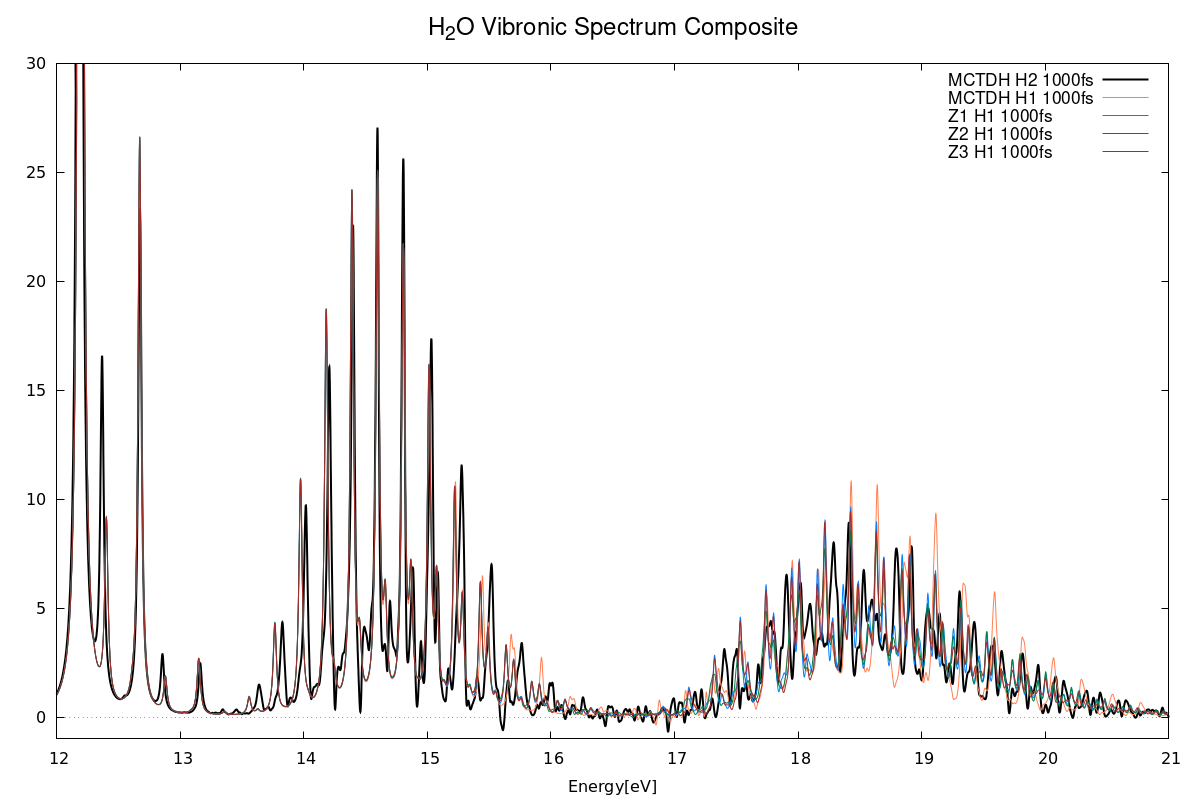
\includegraphics[width=1\columnwidth]{images/Jun_10_H2O_composite.png}
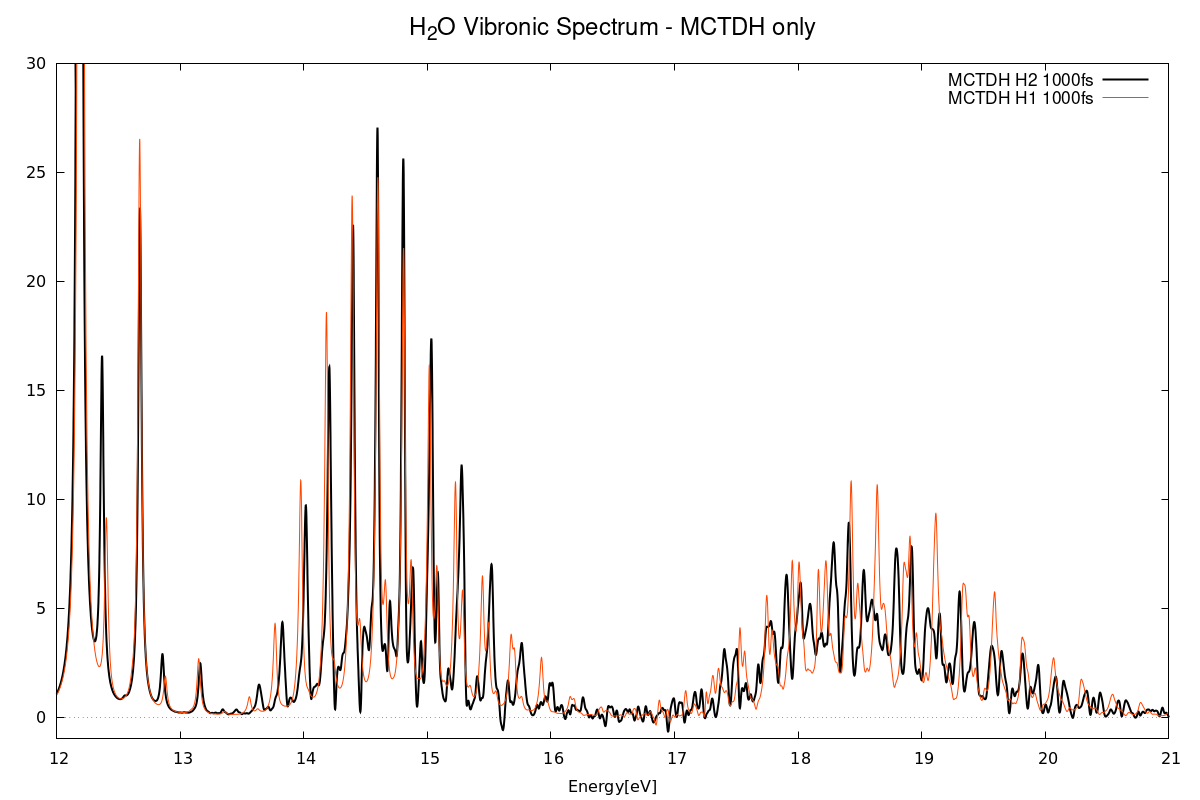
\includegraphics[width=1\columnwidth]{images/Jun_10_H2O_MCTDH_ONLY.png}
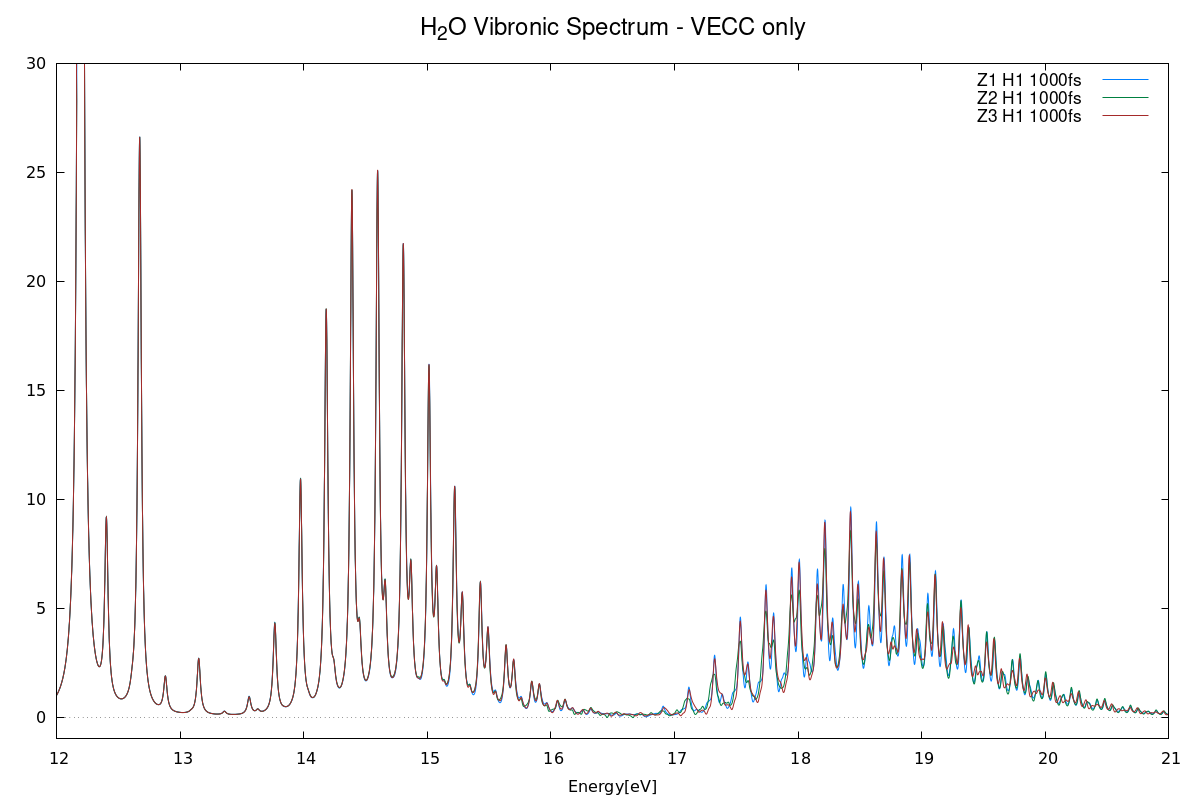
\includegraphics[width=1\columnwidth]{images/Jun_10_H2O_VECC_ONLY.png}
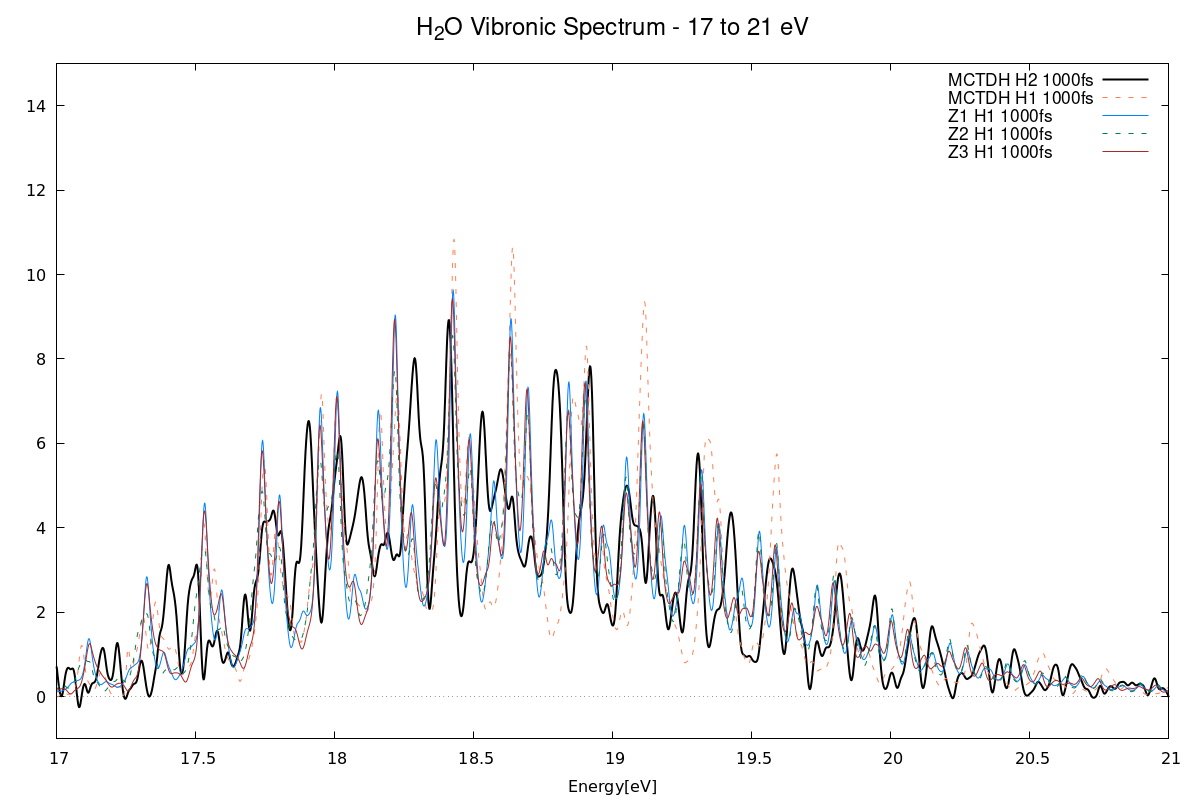
\includegraphics[width=1\columnwidth]{images/Jun_10_H2O_17to21eV.png}

Water was the first molecular species investigated in this research project and was the original test case for running GAMESS calculations. The active space of $H2O^+$ is 6o7e. 

\begin{lstlisting}[language=Fortran, caption=Example H2O Input File]
 $guess  guess=moread norb=24 purify=.t. norder=1 $end
 $mcscf  cistep=gmcci fullnr=.t. finci=mos
         acurcy=1.d-6 maxit=100 $end
 $mrmp   mrpt=gmcpt rdvecs=.f. $end
 $gmcpt  nmofzc=0 nmodoc=1 nmoact=6 nelact=7 stsym(1)=A
         reftyp=ormas nspace=1 mstart(1)=2 mine(1)=7 maxe(1)=7
         kstate(1)=1,1,1
         wstate(1)=1,1,1
         iwgt=0 thrwgt=-1.0 krot=.f. kszdoe=.f. knospn=.f.
         thrde=-1.0 edshft=0.02 $end
 $data
 H2O 3 state diabatization
 C1
 O           8.0   0.0000000000   0.0000000000  -0.0529241093
 H           1.0   0.7493169121  -0.0000000000   0.5549604347
 H           1.0  -0.7493169121   0.0000000000   0.5549604347
\end{lstlisting}

\begin{lstlisting}
    nmofzc=0 nmodoc=1 nmoact=6 nelact=7 mstart(1)=2 icharg = 1 mult = 2 gbasis = ccd state(1) = 4
\end{lstlisting}


% add short description of file
% show table with Hamiltonian parameters
% show image of molecule? (probably unnecessary)
% show spectra from MCTDH and VECC (maybe show constant, linear, quadratic, SOC?)
% discuss the results? are they identical, good this system was just top test xyz, and it behaved as we expected.

% ------------------------------------------------------------------------------------
\subsection{CH2O}
blah
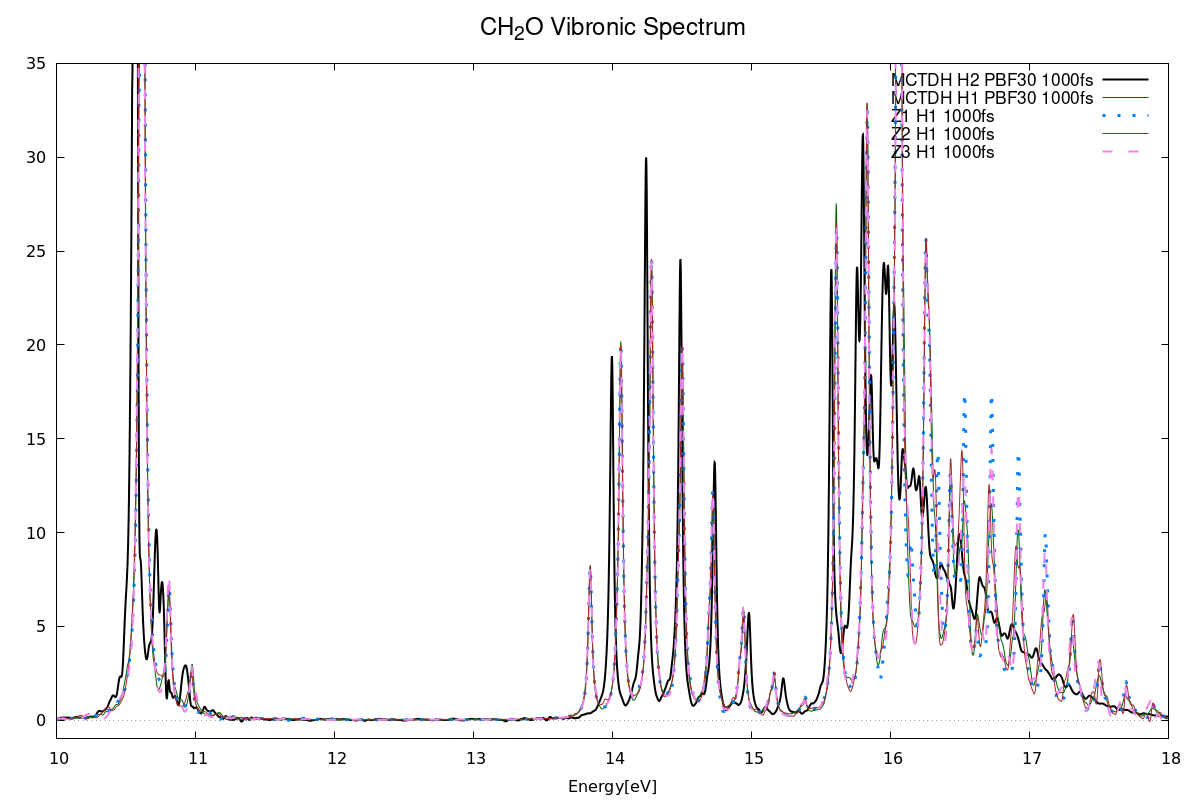
\includegraphics[width=1\columnwidth]{images/Jun_13_CH2O_composite.png}
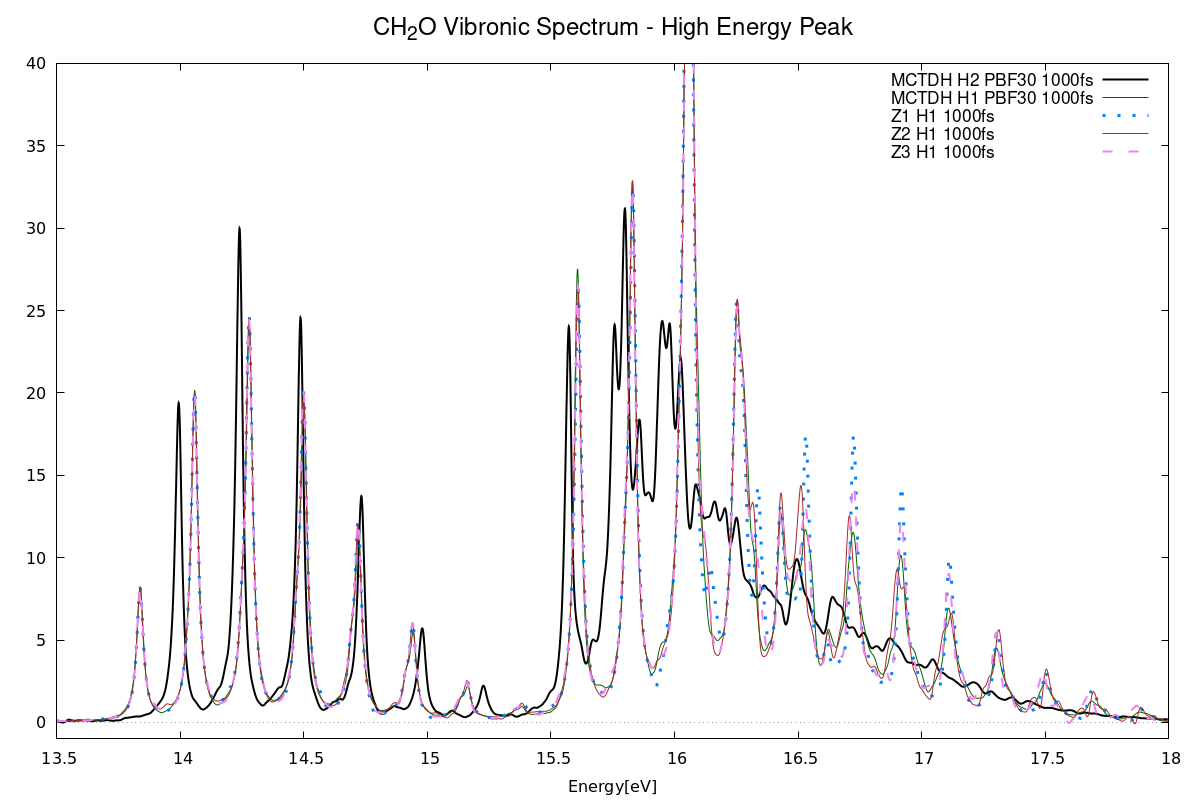
\includegraphics[width=1\columnwidth]{images/Jun_13_CH2O_highpeak.png}
% TEXT MUST ALWAYS FOLLOW THE IMAGES TO ENSURE THERE ARE NO RANDOM BLANK PAGES!!
add short description of file
show table with Hamiltonian parameters
show image of molecule? (progbably unnnecessary)
show spectra from MCTDH and VECC (maybe show constant, linear, quadratic, SOC?)
discuss the results? are they identical, good this system was just top test xyz, and it behaved as we expected.

% ------------------------------------------------------------------------------------
\subsection{NH3}
blahj
\begin{figure}[H]
    \center
    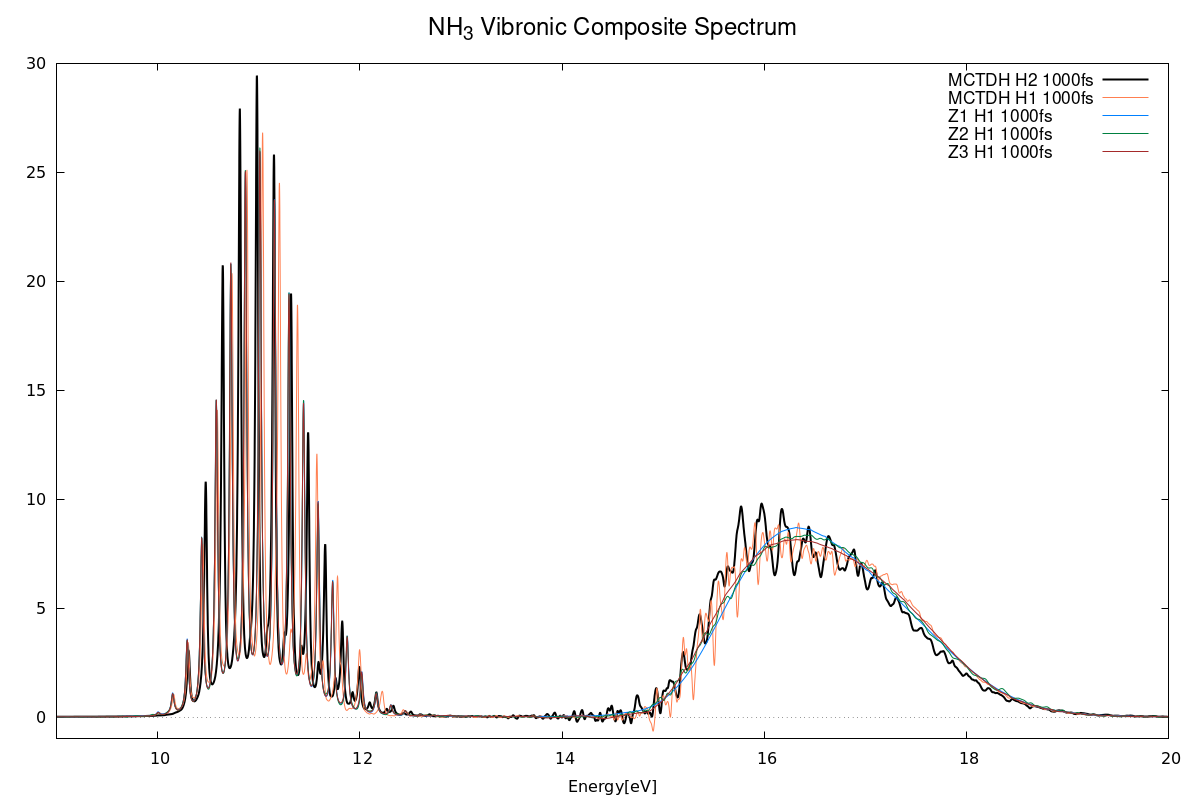
\includegraphics[width=1\columnwidth]{images/Jun_10_NH3_composite.png}
    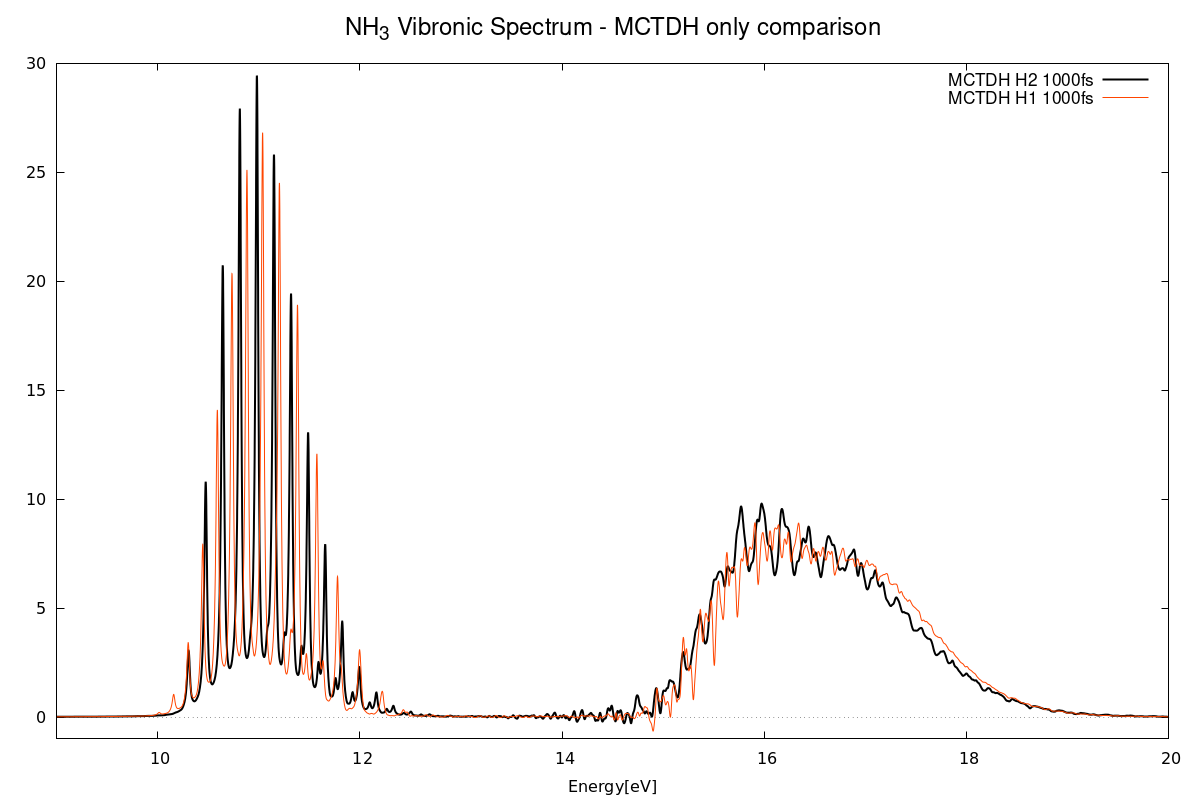
\includegraphics[width=1\columnwidth]{images/Jun_10_NH3_MCTDH_ONLY.png}
\end{figure}
\begin{figure}[H]
    \center
    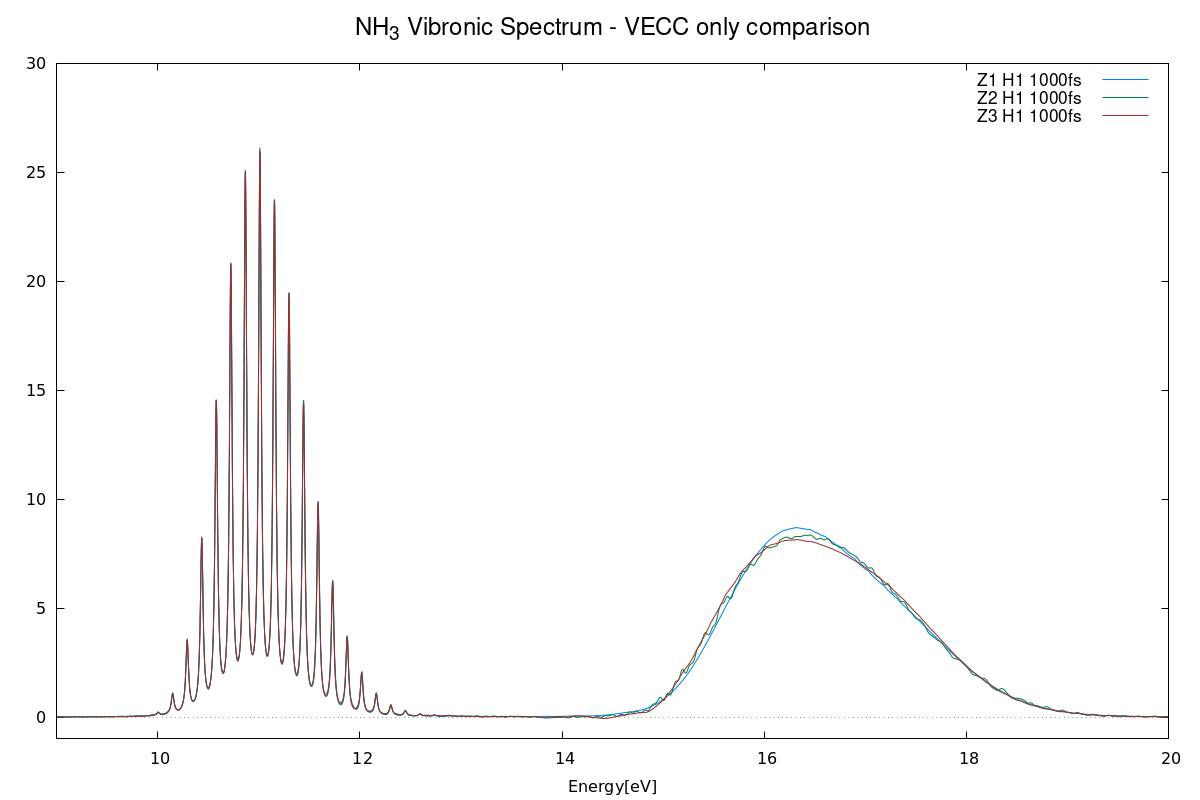
\includegraphics[width=1\columnwidth]{images/Jun_10_NH3_VECC_ONLY.png}
    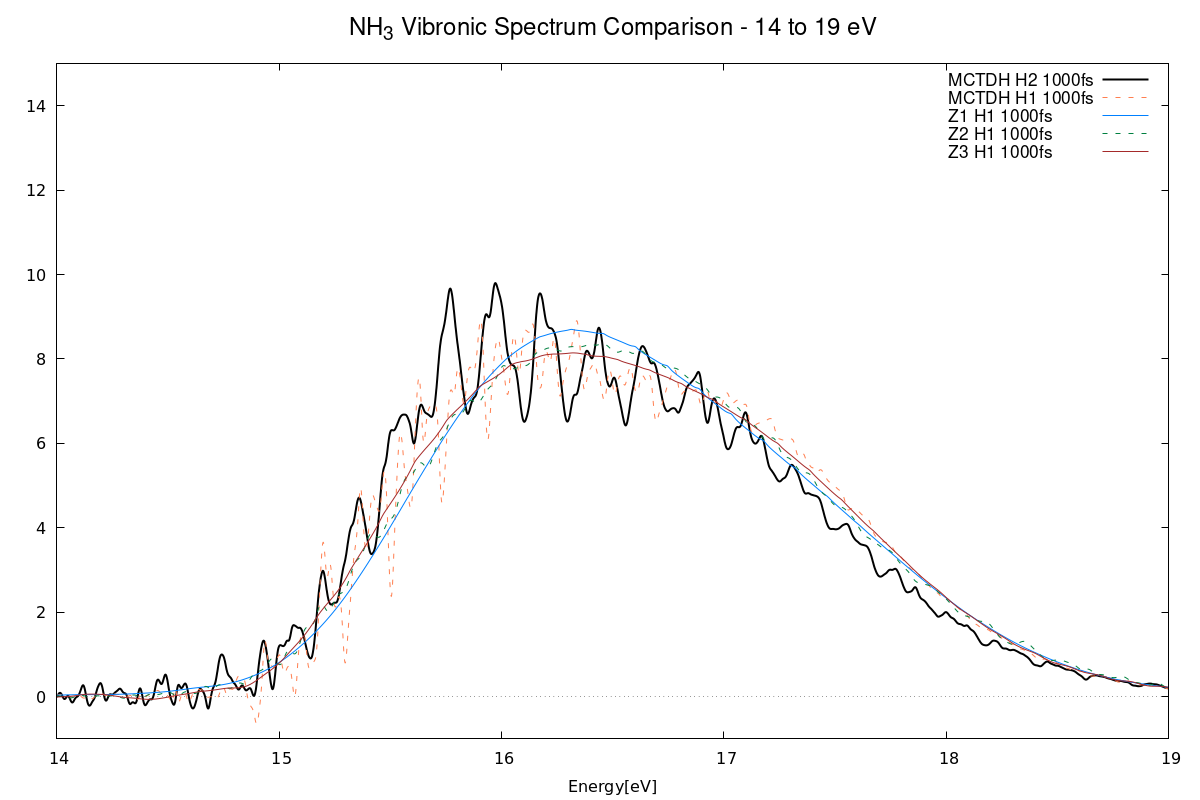
\includegraphics[width=1\columnwidth]{images/Jun_10_NH3_14to19eV.png}
\end{figure}

add short description of file
show table with Hamiltonian parameters
show image of molecule? (progbably unnnecessary)
show spectra from MCTDH and VECC (maybe show constant, linear, quadratic, SOC?)
discuss the results? are they identical, good this system was just top test xyz, and it behaved as we expected.

% ------------------------------------------------------------------------------------
\subsection{PH3}
blah
\begin{figure}[H]
    \center
    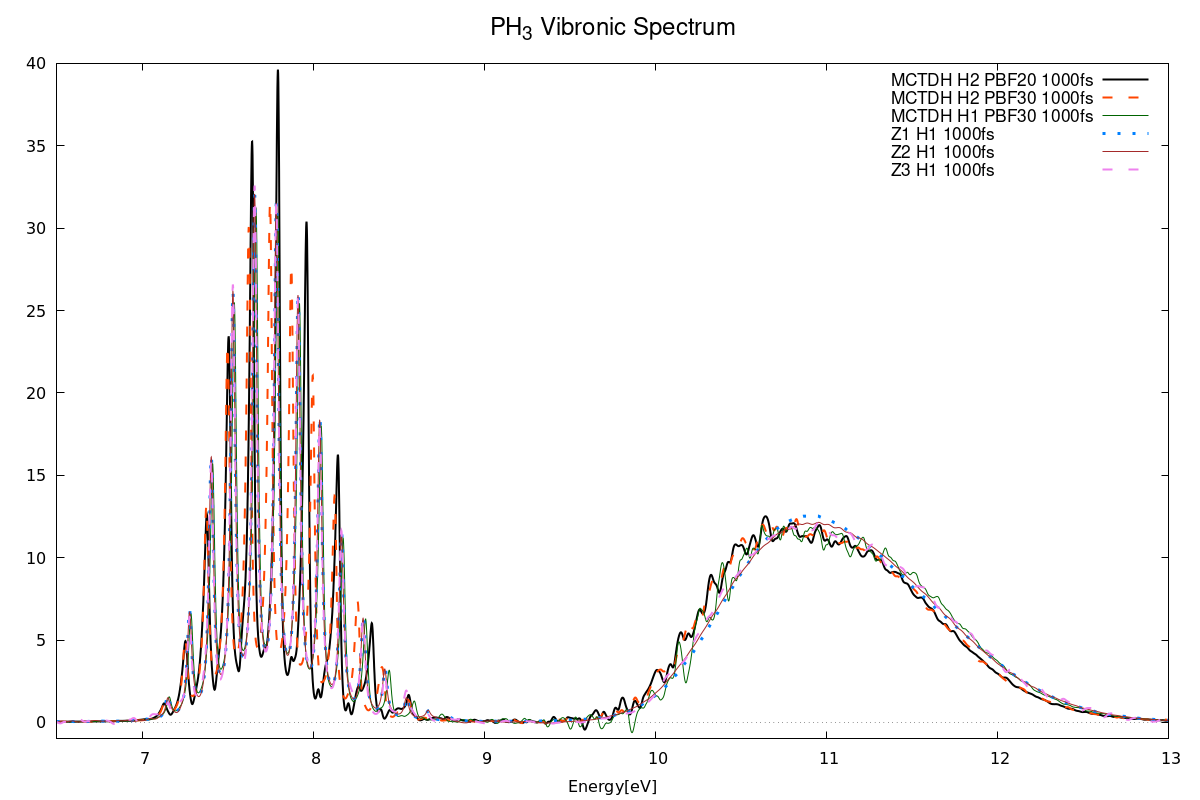
\includegraphics[width=1\columnwidth]{images/Jun_12_PH3_composite.png}
    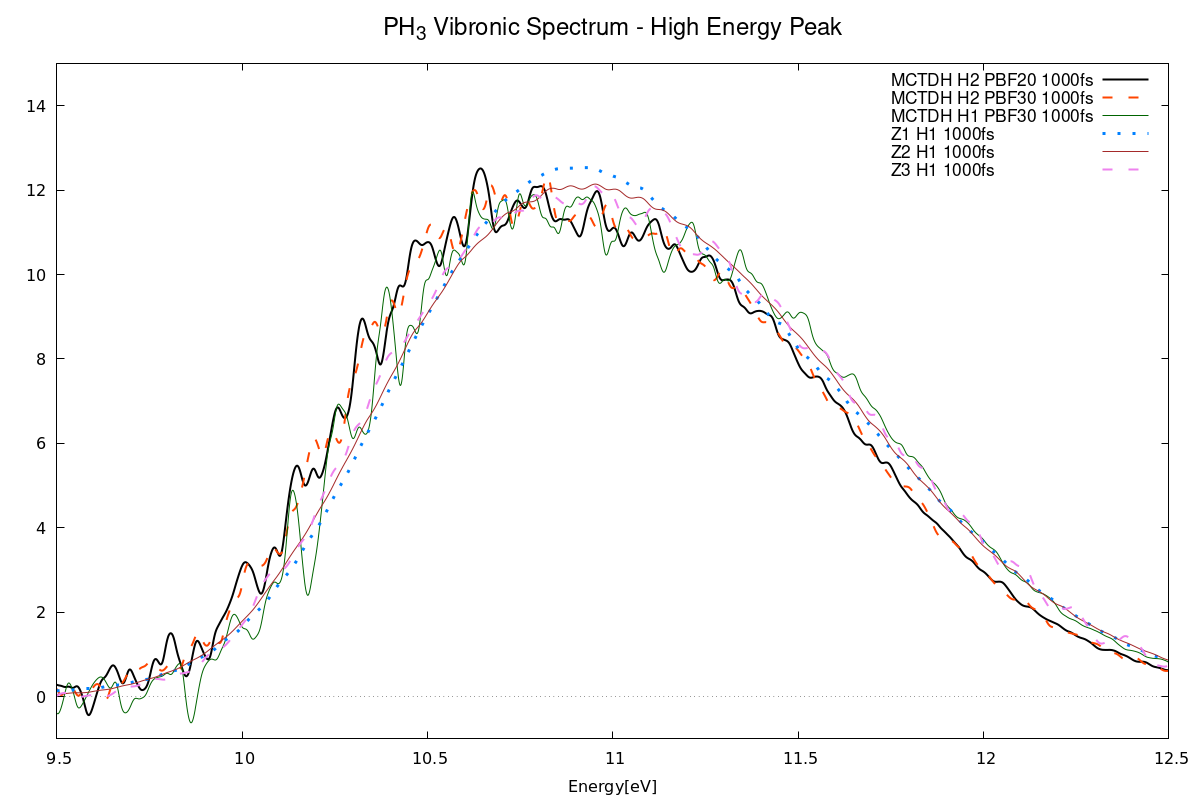
\includegraphics[width=1\columnwidth]{images/Jun_12_PH3_highpeak.png}
\end{figure}

% ------------------------------------------------------------------------------------
% ------------------------------------------------------------------------------------
\section{Complex systems}
% ------------------------------------------------------------------------------------
%A paragraph that talks about the three systems. 
As we explained in (section intro) transition metal complexes are of high importance because <some reason>.
We primarily focused on CoF3, RhF3 and Fe(CO)5 beacuse of <some reason>.
The two smaller systems (CoF3, RhF3) are good for benchmarking the model generation as well as fine-tuning the calculation parameters for MCTDH and VECC.
The large system (Fe(CO)5) is expected to be very difficult and has only some citation of a paper and demonstrate how its real tough and scary

To align VECC and MCTDH, it was a monumental task to get things right. We had to consult with Dieter Meyer! Finetuning. Hurdles as Marcel would say...


% ------------------------------------------------------------------------------------
\subsection{CoF3}
blah, no empty page \\
% OLD SPECTRA
% 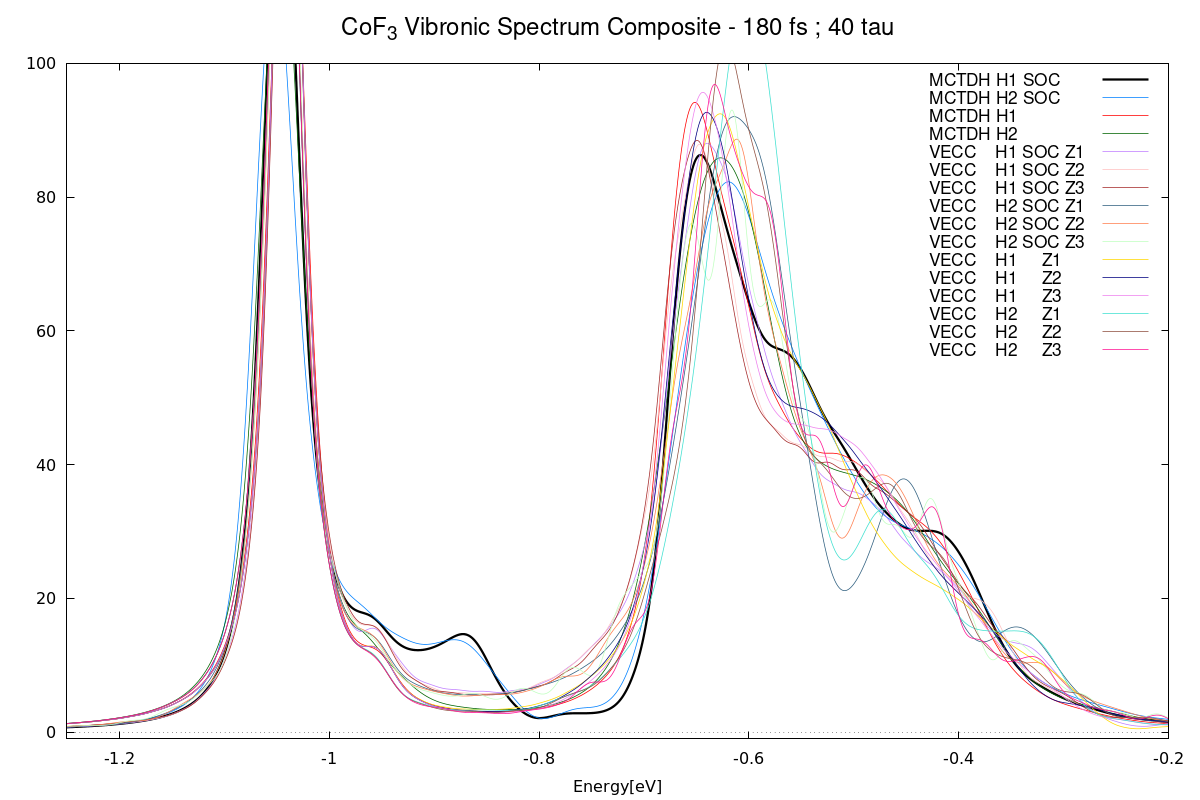
\includegraphics[width=1\columnwidth]{images/COF3_FINAL/Jun_24_CoF3_waterfall_composite.png}
% 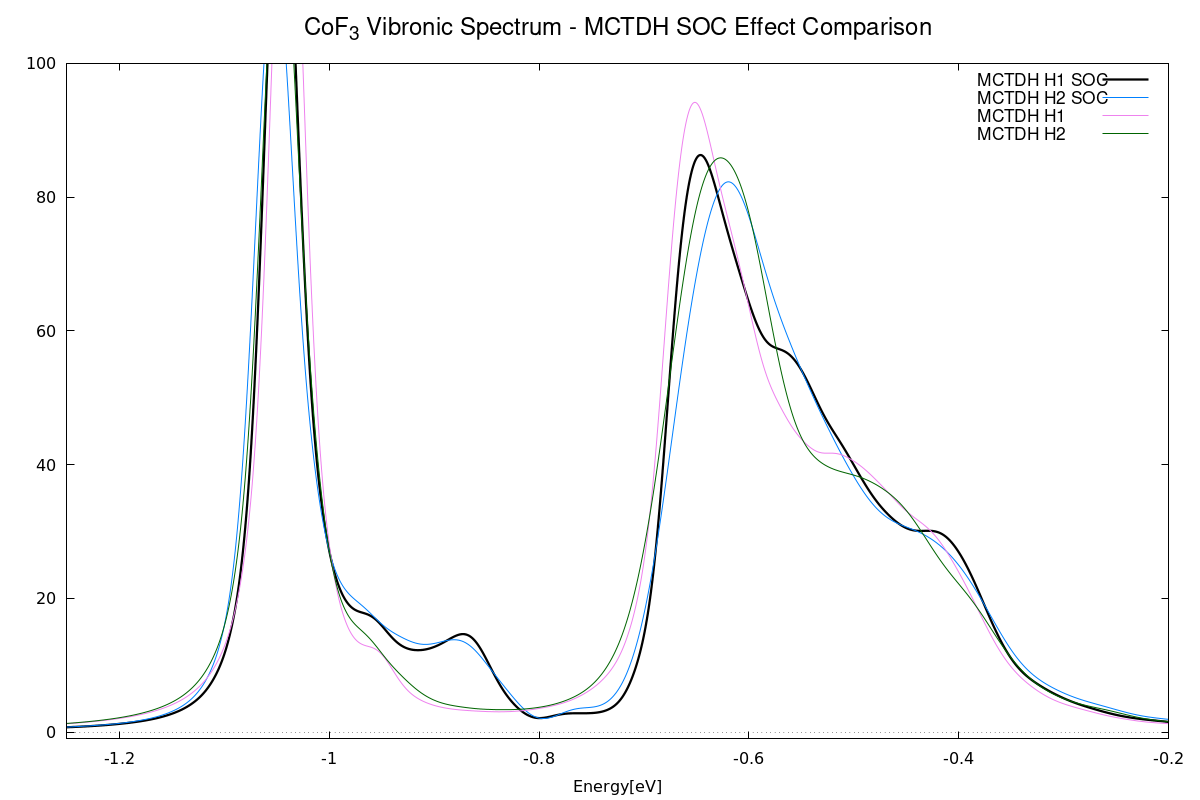
\includegraphics[width=1\columnwidth]{images/COF3_FINAL/Jun_24_CoF3_MCTDH_SOC.png}
% 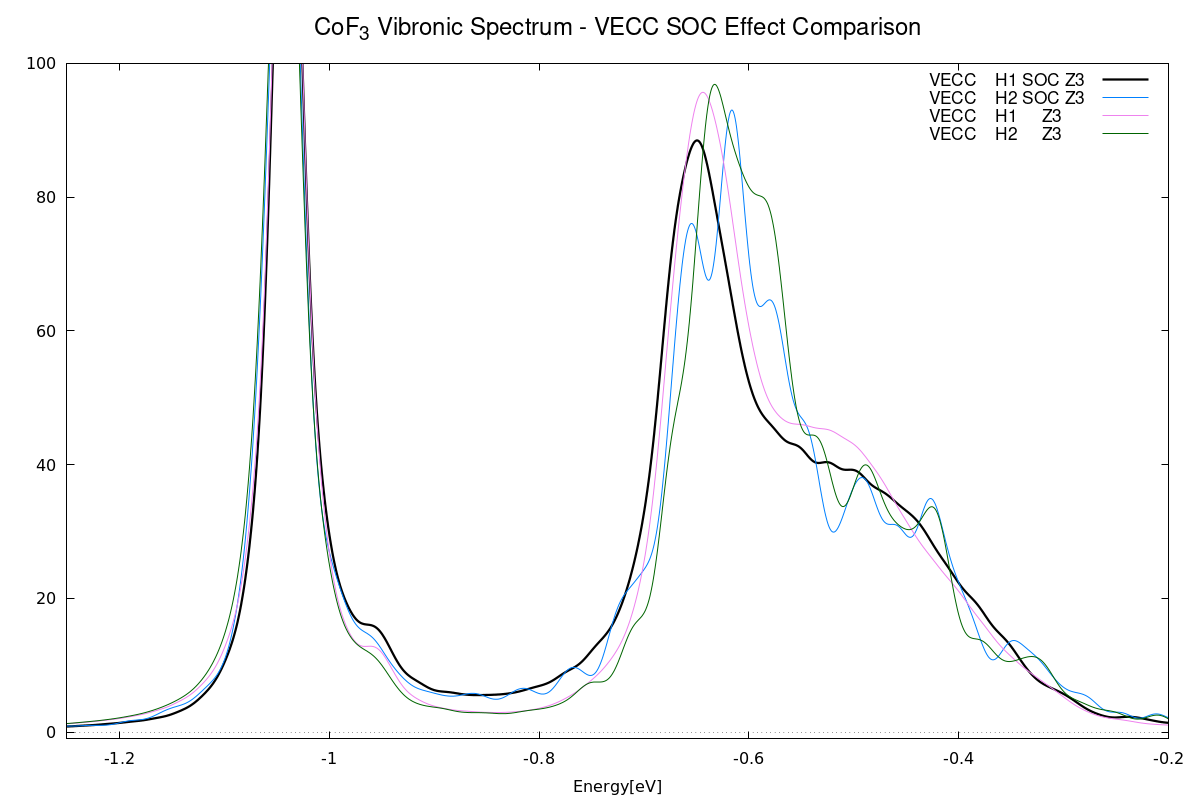
\includegraphics[width=1\columnwidth]{images/COF3_FINAL/Jun_24_CoF3_VECC_SOC.png}
% 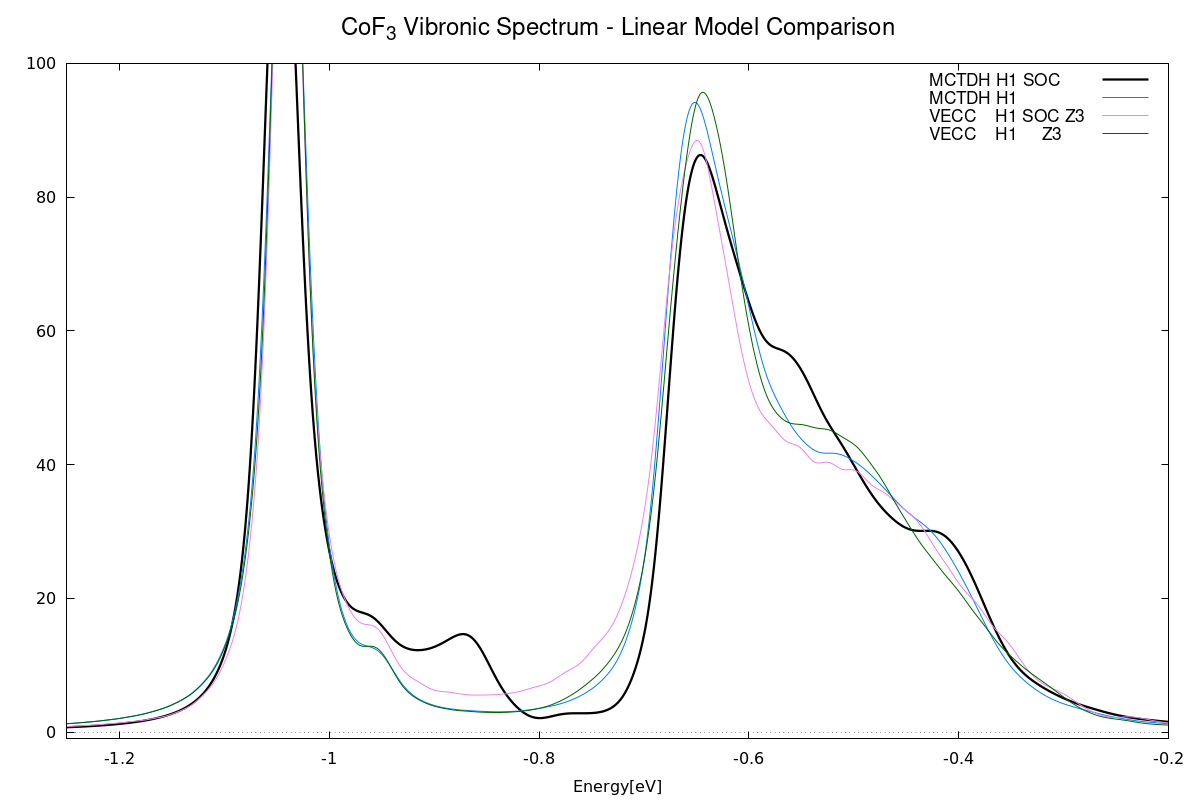
\includegraphics[width=1\columnwidth]{images/COF3_FINAL/Jun_24_CoF3_Linears.png}
% 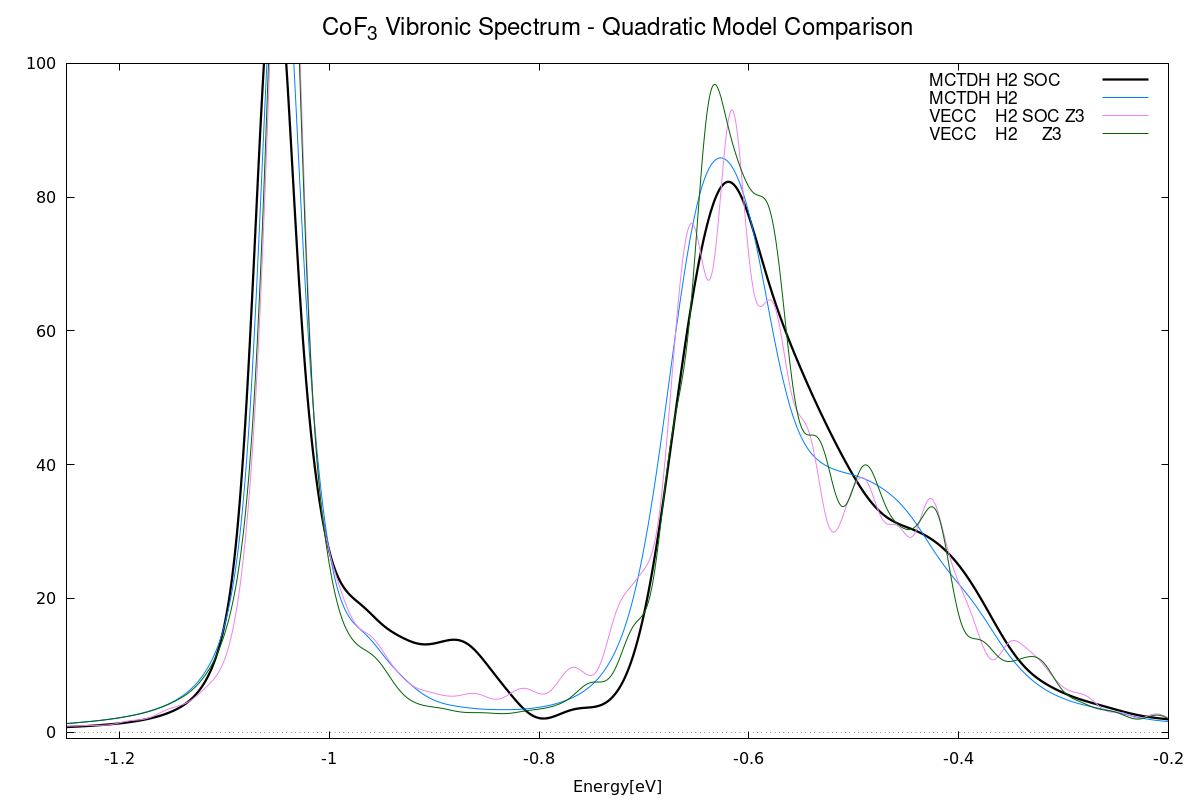
\includegraphics[width=1\columnwidth]{images/COF3_FINAL/Jun_24_CoF3_Quadratics.png}
% 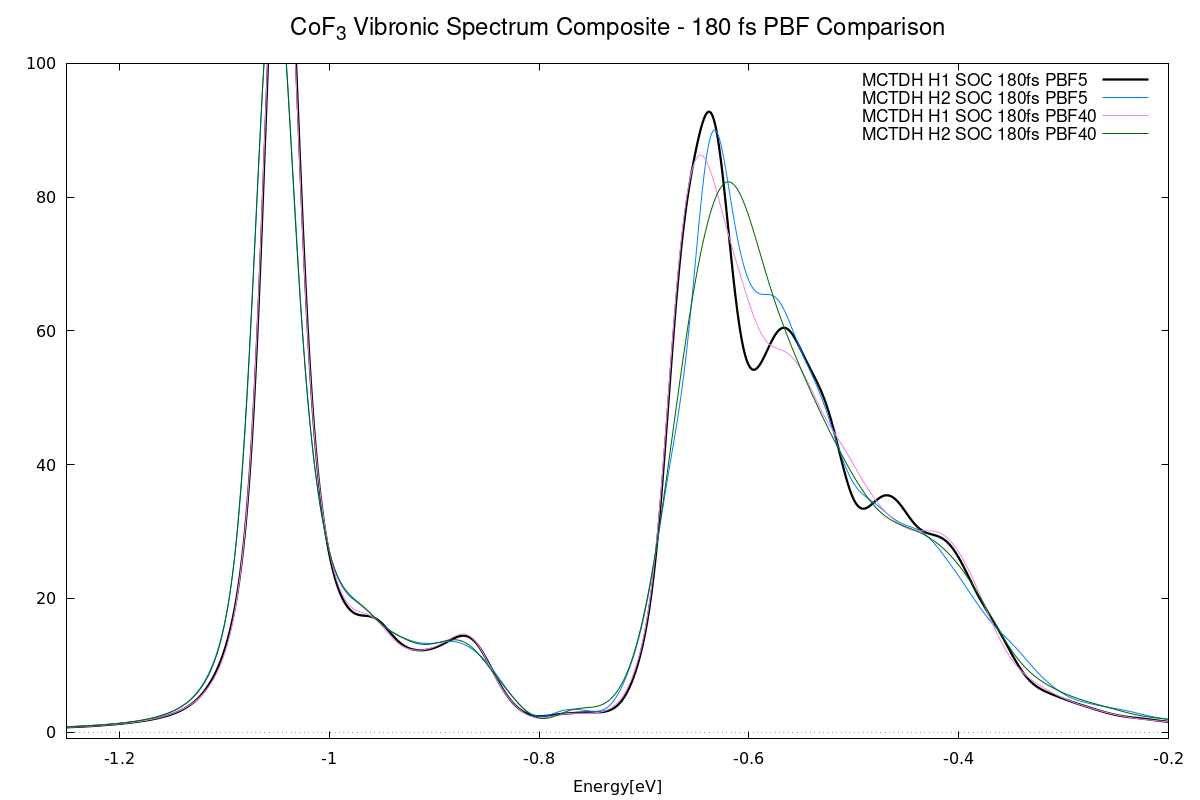
\includegraphics[width=1\columnwidth]{images/COF3_FINAL/Jun_24_CoF3_PBF_180fs.png}
% 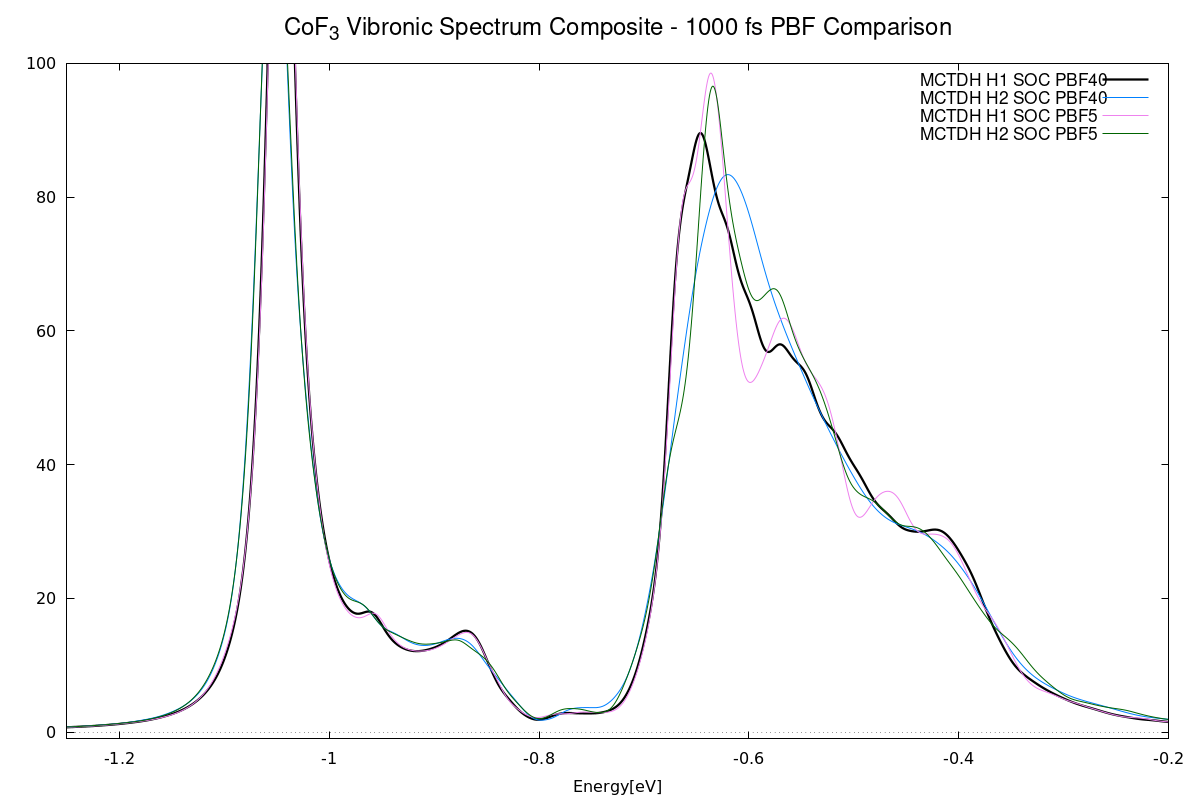
\includegraphics[width=1\columnwidth]{images/COF3_FINAL/Jun_24_CoF3_PBF_1000fs.png}

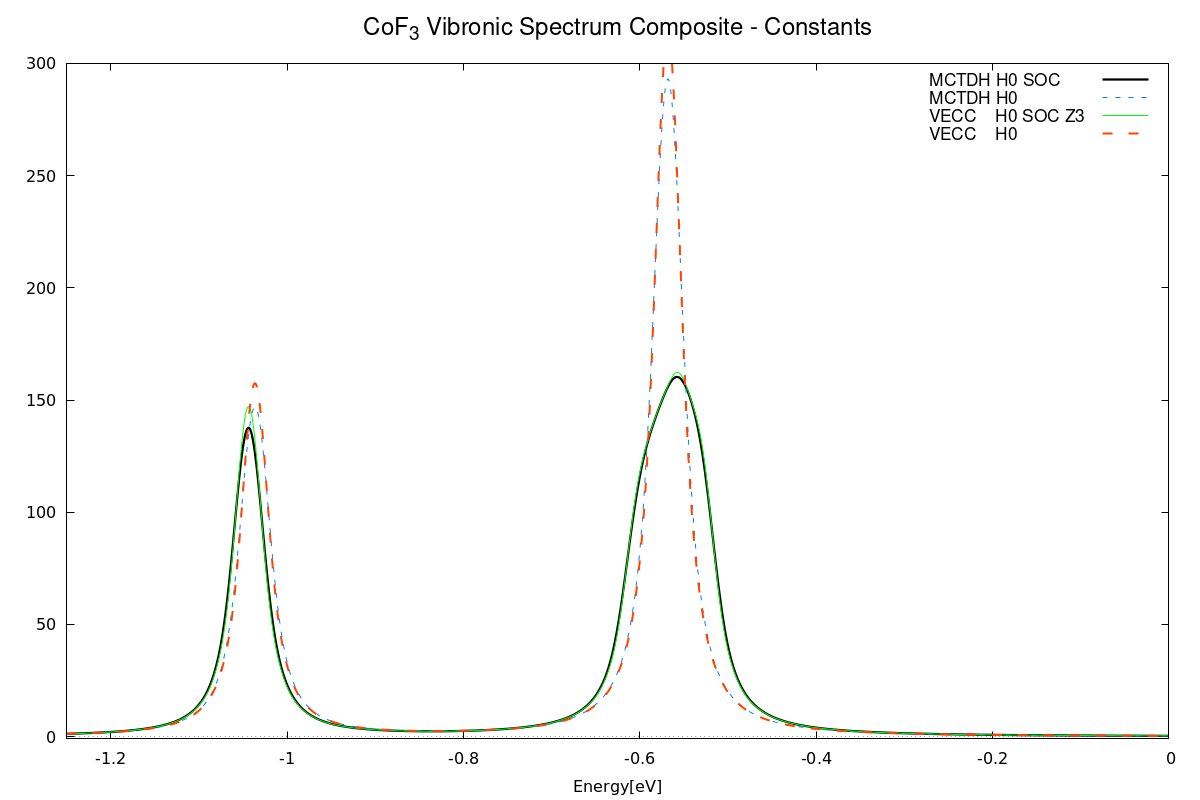
\includegraphics[width=1\columnwidth]{images/COF3_FINAL/Jul_08_CoF3_constants.png}
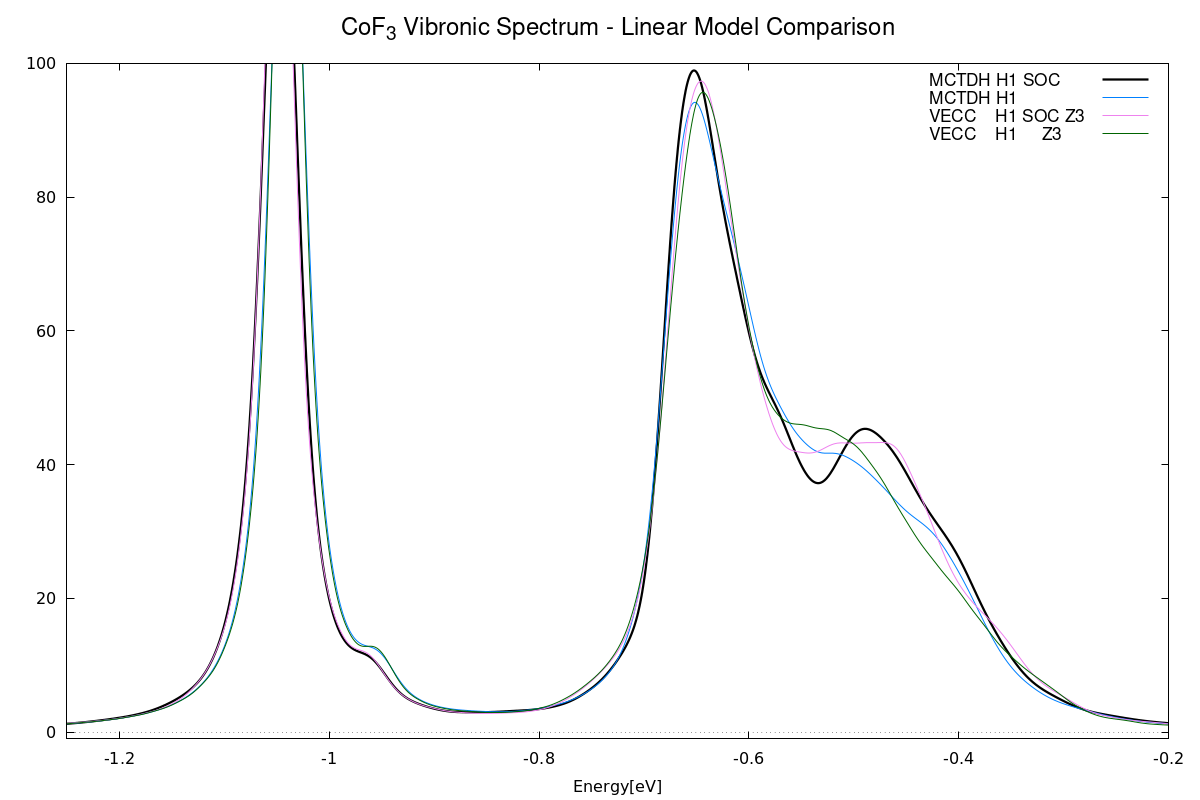
\includegraphics[width=1\columnwidth]{images/COF3_FINAL/Jul_08_CoF3_Linears.png}
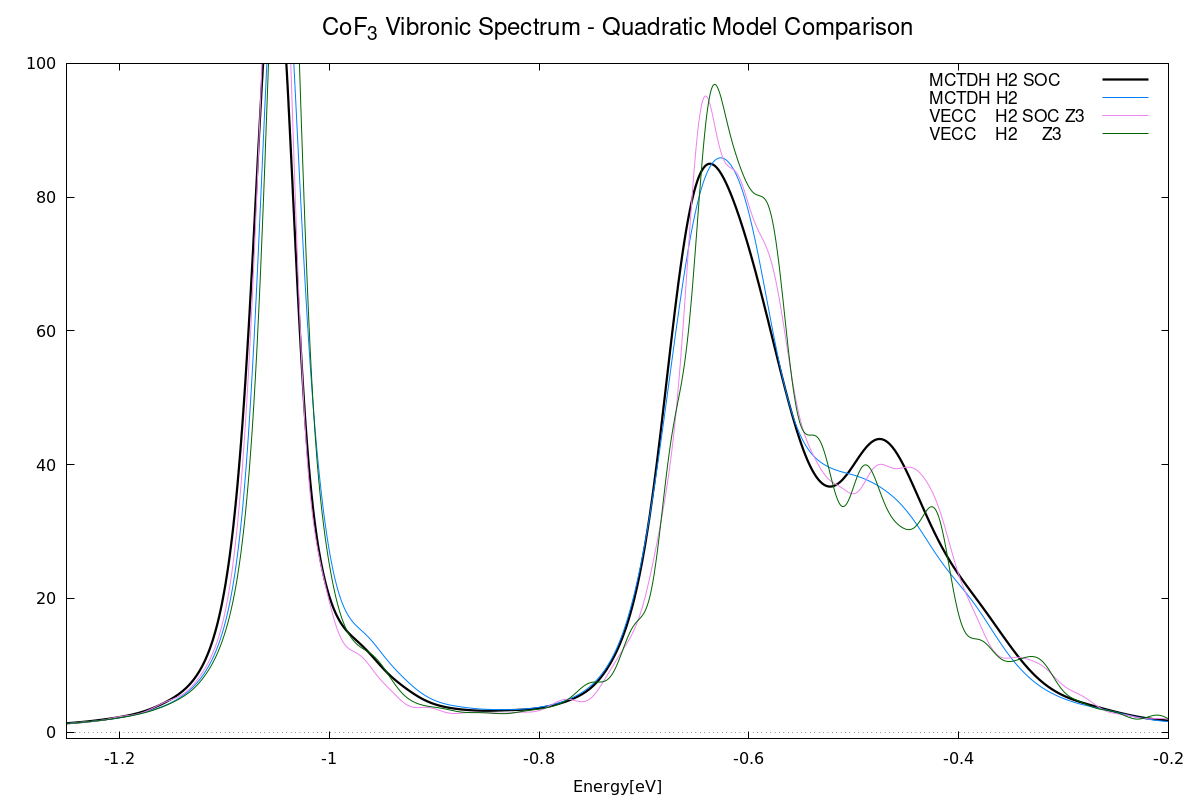
\includegraphics[width=1\columnwidth]{images/COF3_FINAL/Jul_08_CoF3_Quadratics.png}
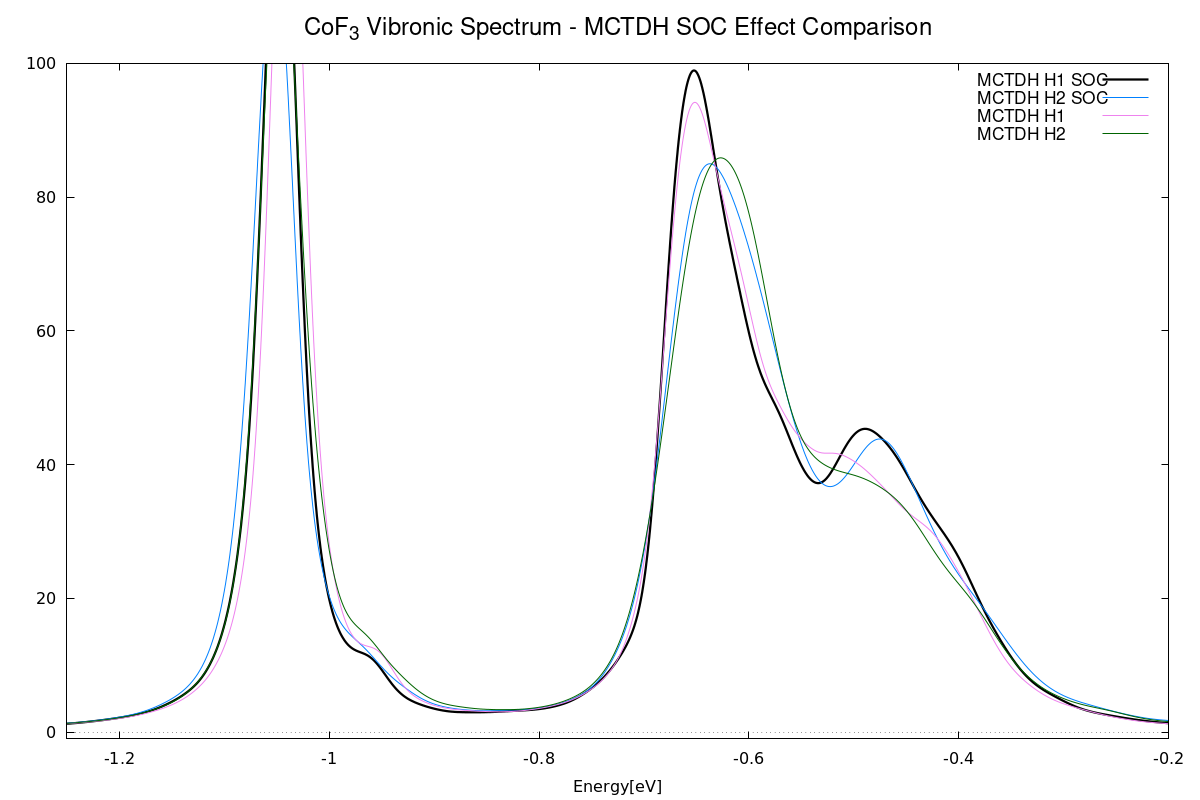
\includegraphics[width=1\columnwidth]{images/COF3_FINAL/Jul_08_CoF3_MCTDH_SOC.png}
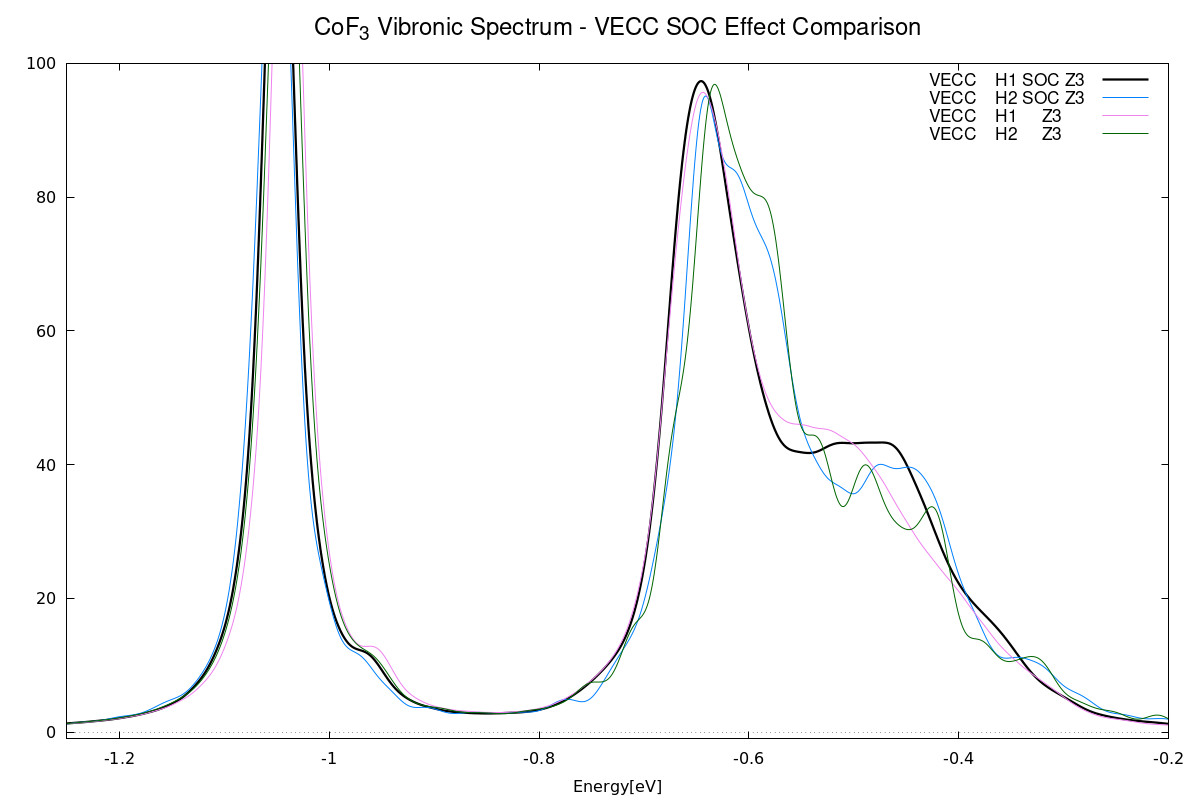
\includegraphics[width=1\columnwidth]{images/COF3_FINAL/Jul_08_CoF3_VECC_SOC.png}
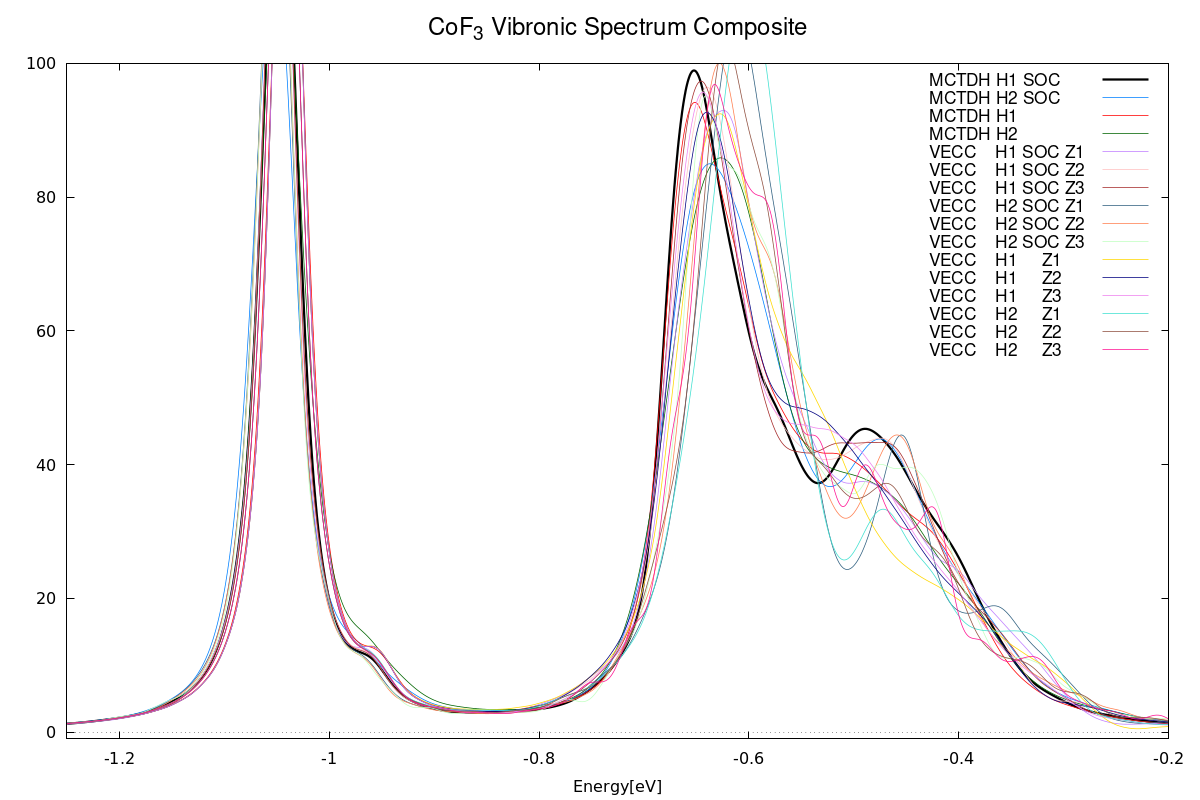
\includegraphics[width=1\columnwidth]{images/COF3_FINAL/Jul_08_CoF3_waterfall_composite.png}

% Comparison of Tau \\
% 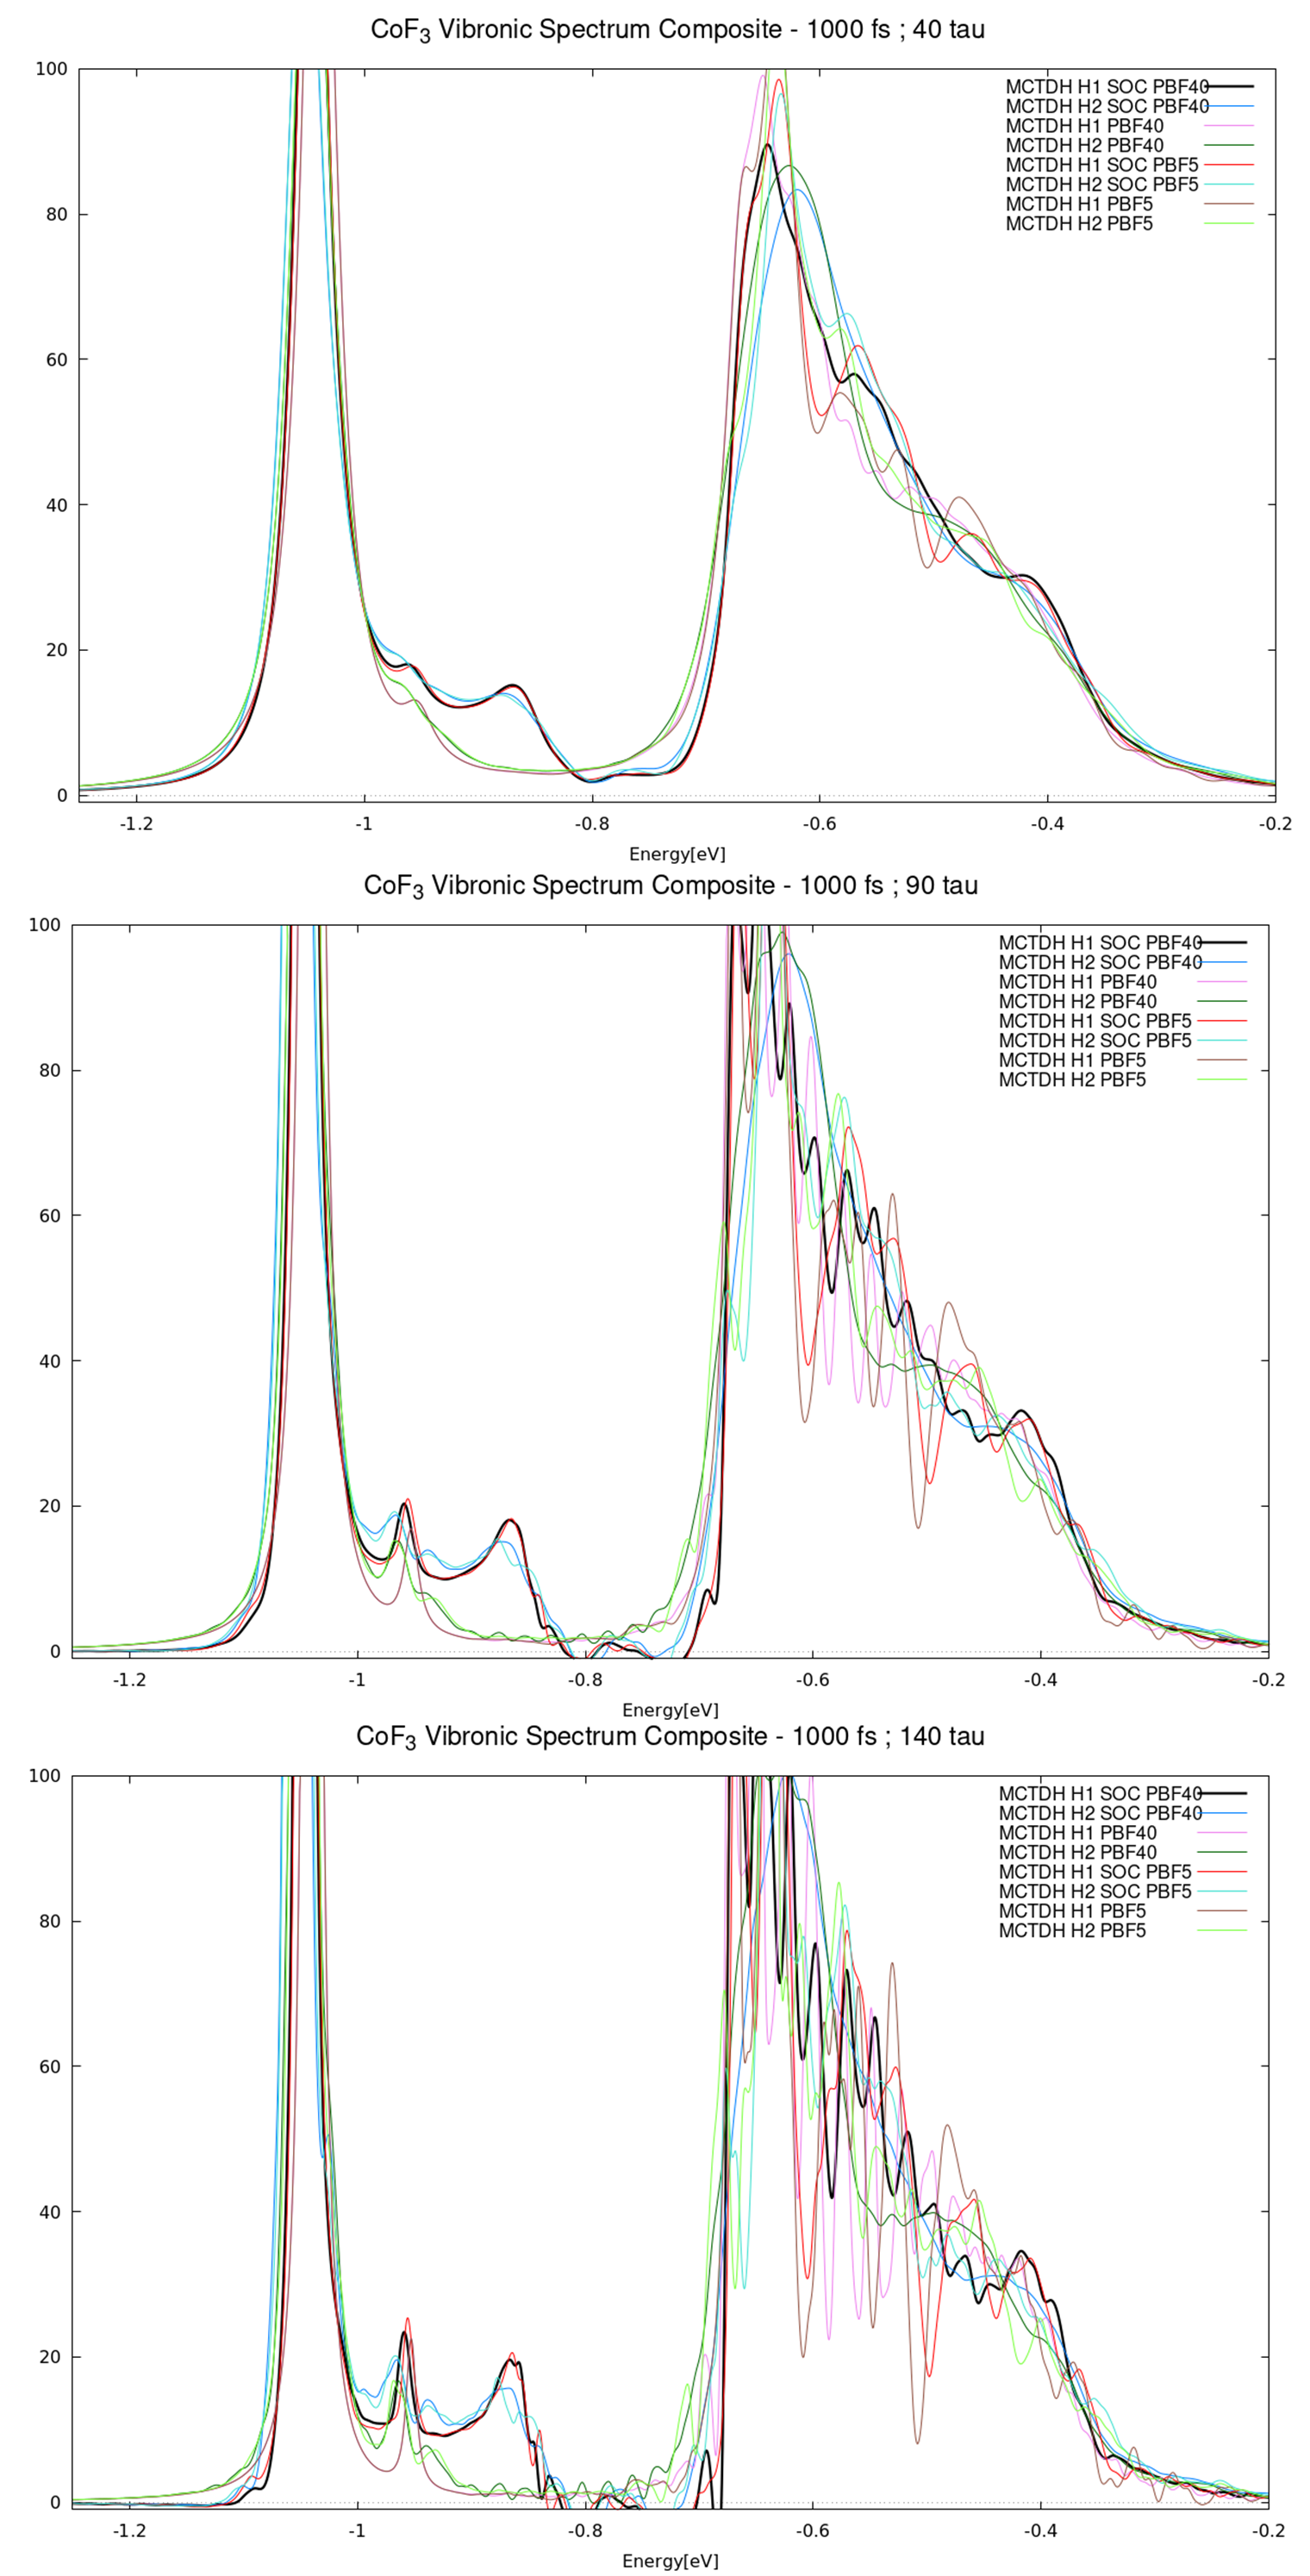
\includegraphics[width=0.7\columnwidth]{images/TAU_COMPARE_VERT.png}
% \begin{figure}[H]
%     \center
%     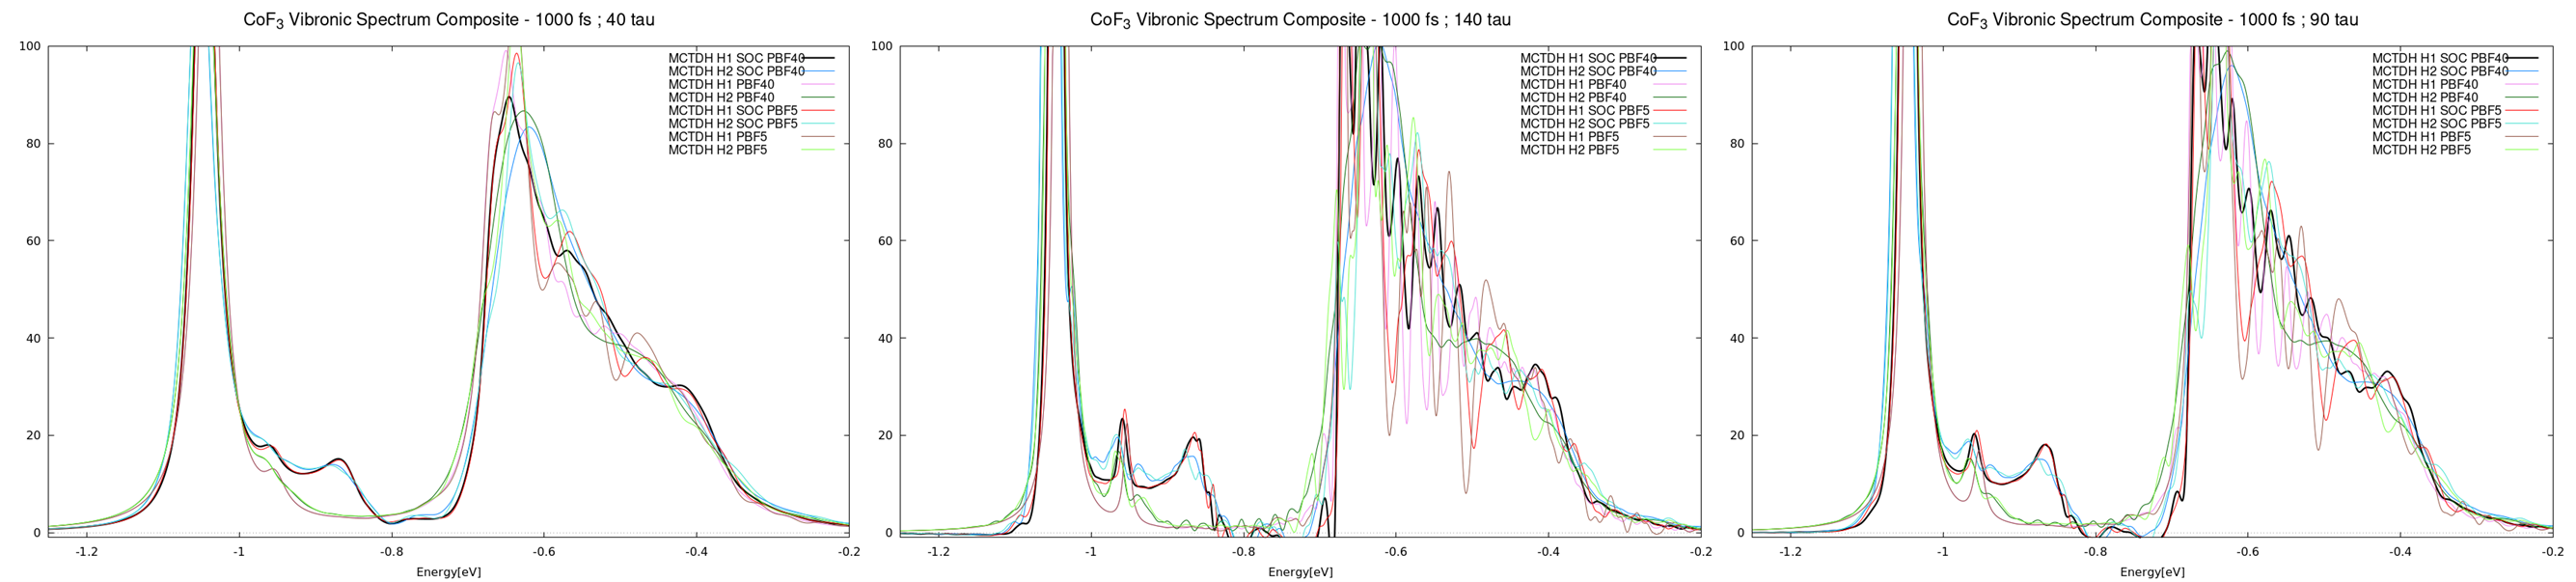
\includegraphics[width=1.3\columnwidth]{images/TAU_COMPARE.png}
% \end{figure}
% 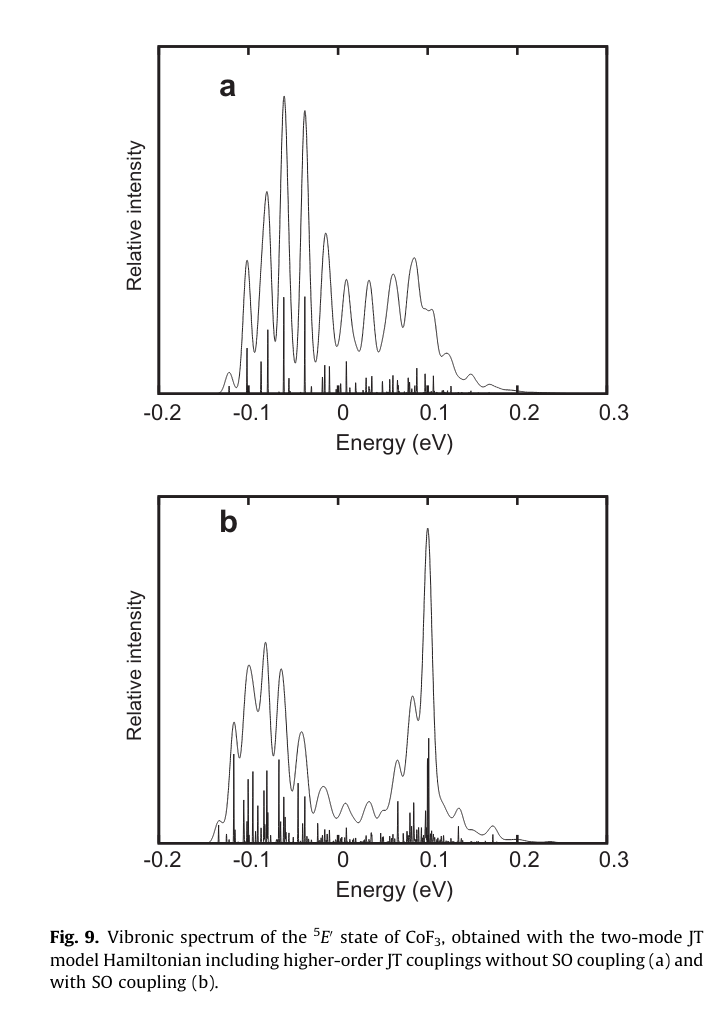
\includegraphics[width=1\columnwidth]{images/COMPARE_EXPERIMENTAL/CoF3_simulation_mondal.PNG}
% taken from "Jahn–Teller and spin–orbit coupling effects in transition-metal trifluorides" //

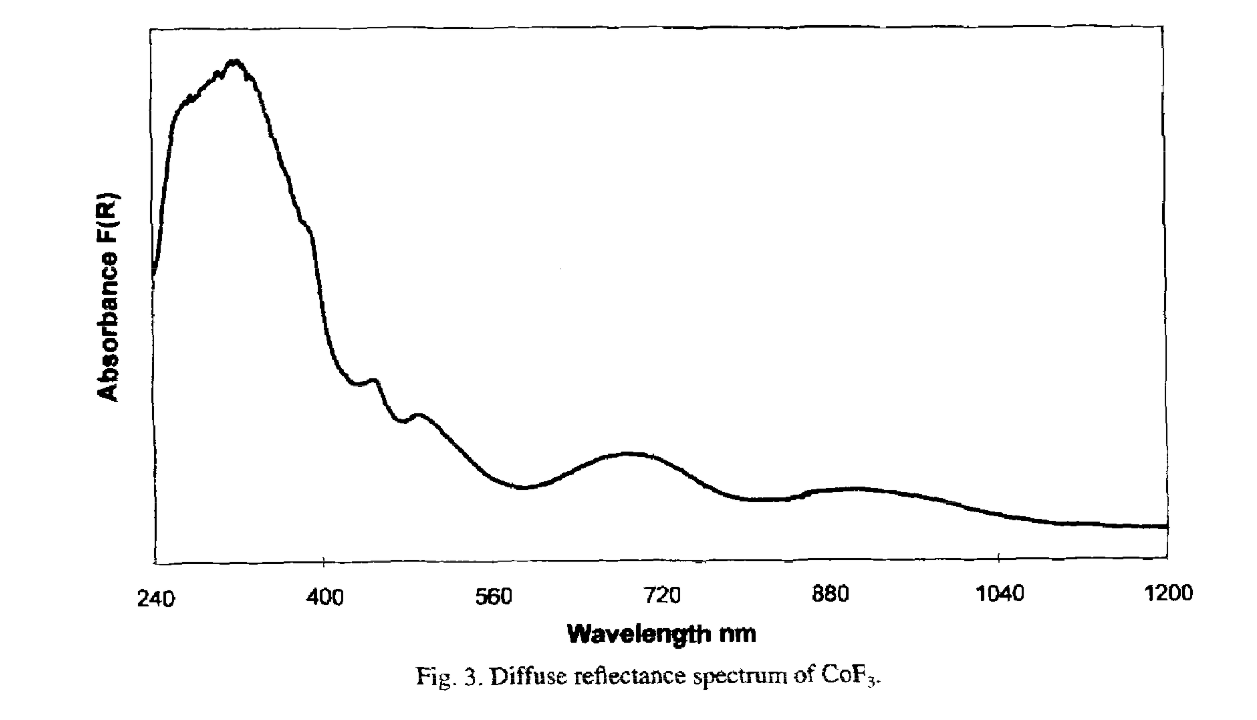
\includegraphics[width=1\columnwidth]{images/COMPARE_EXPERIMENTAL/CoF3_reflectance_hector.PNG}
taken from "UV-visible spectroscopic studies of group 8-10 metal trifluorides" //



add short description of file
show table with Hamiltonian parameters
show image of molecule? (progbably unnnecessary)
show spectra from MCTDH and VECC (maybe show constant, linear, quadratic, SOC?)
discuss the results? are they identical, good this system was just top test xyz, and it behaved as we expected.
% ------------------------------------------------------------------------------------
\subsection{RhF3}
blah
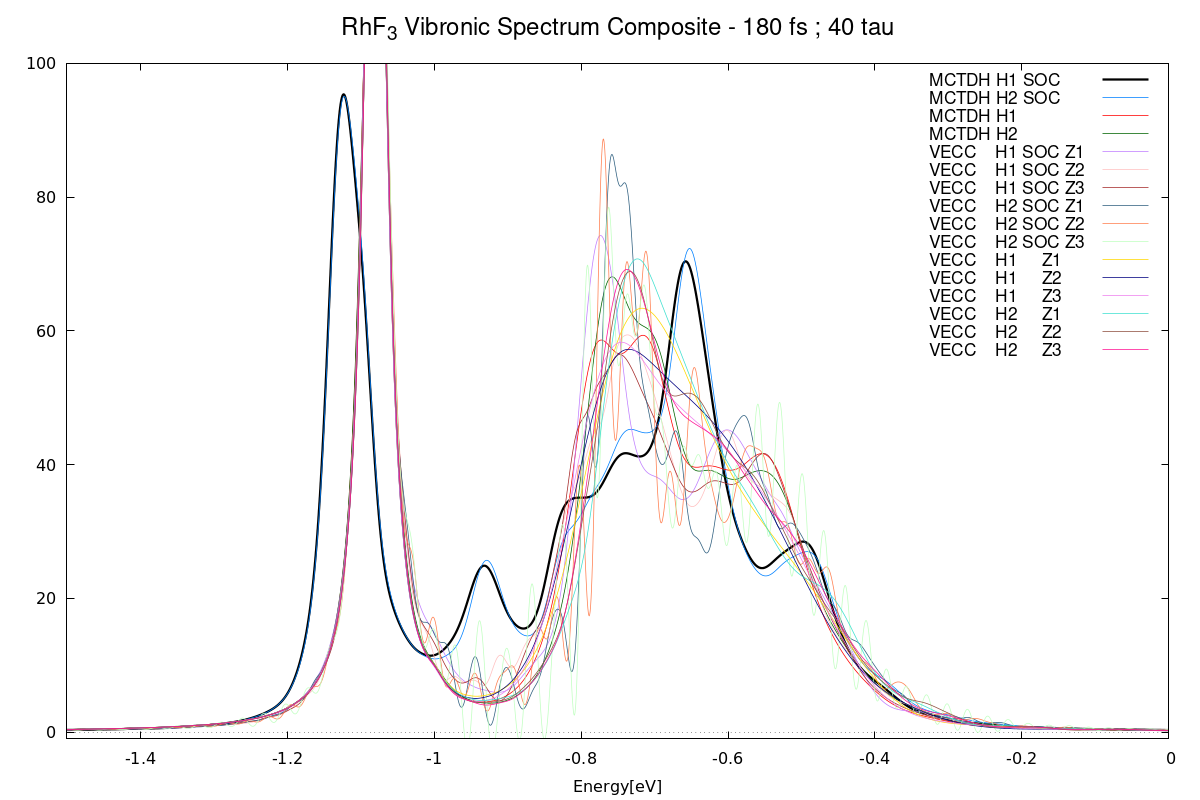
\includegraphics[width=1\columnwidth]{images/RhF3_FINAL/Jun_24_RhF3_waterfall_composite.png}
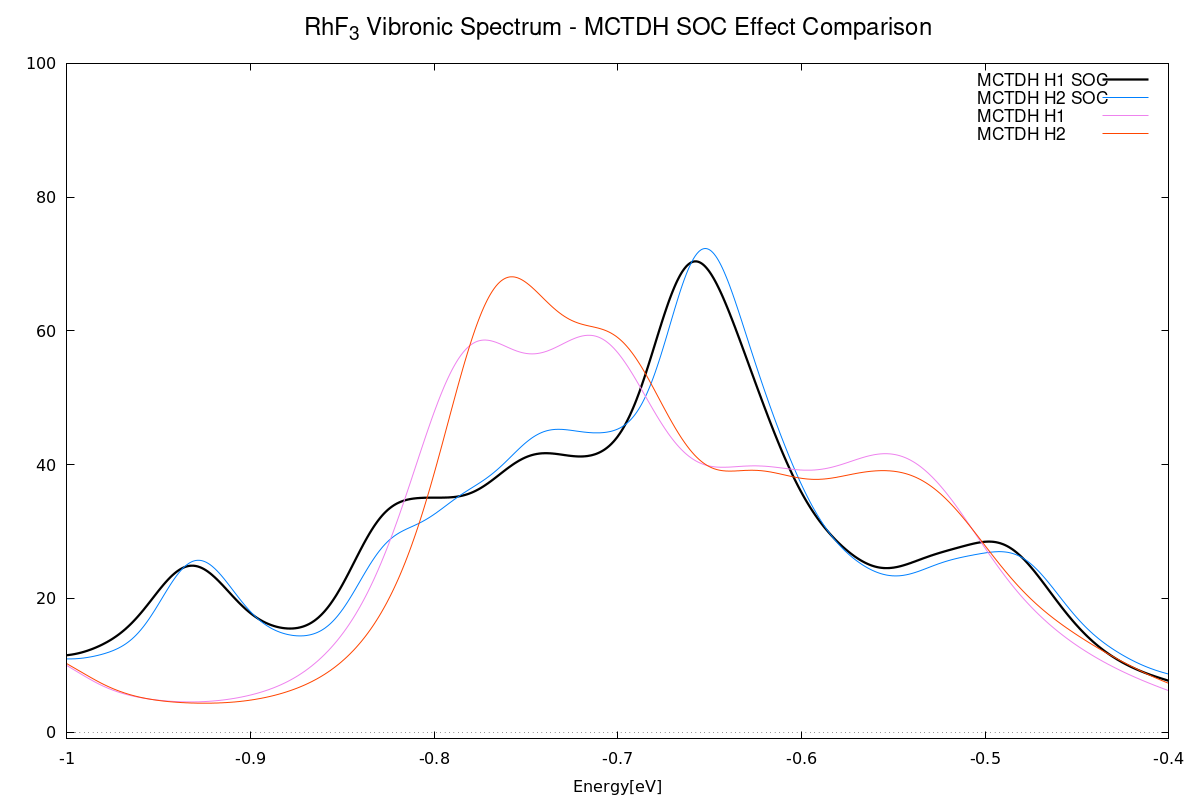
\includegraphics[width=1\columnwidth]{images/RhF3_FINAL/Jun_24_RhF3_MCTDH_SOC.png}
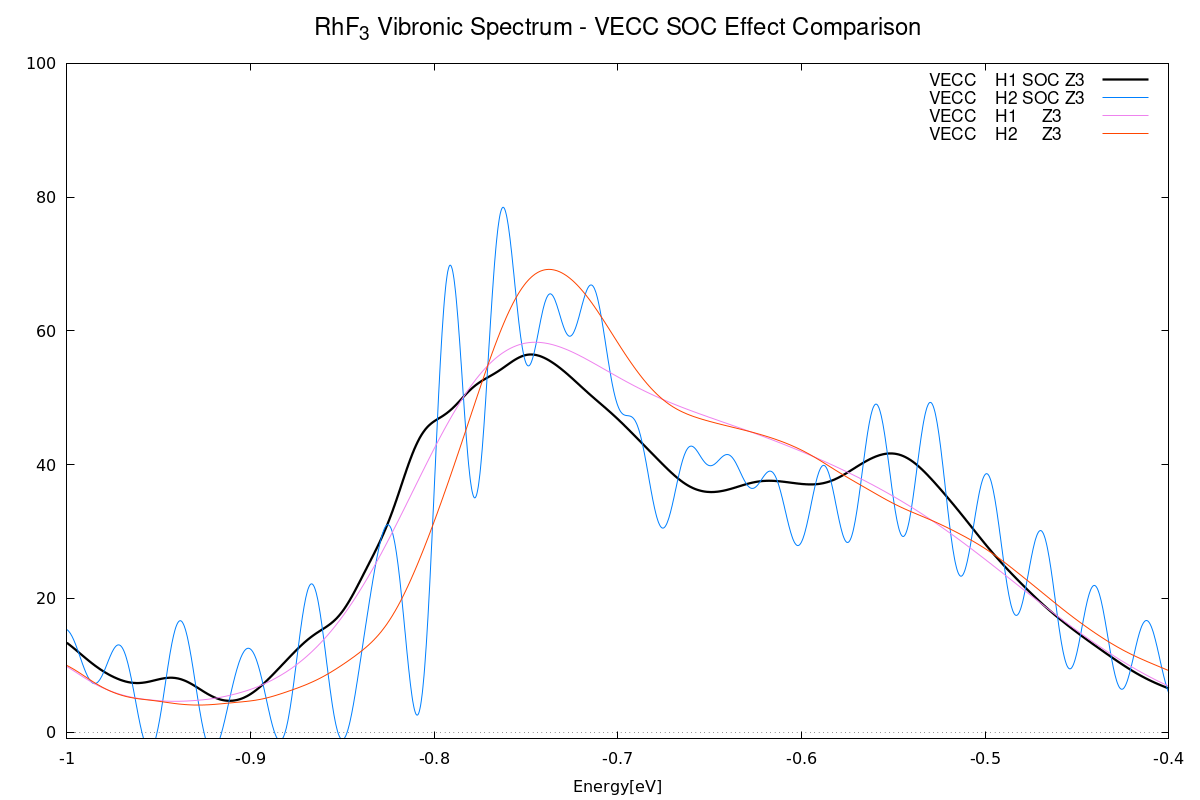
\includegraphics[width=1\columnwidth]{images/RhF3_FINAL/Jun_24_RhF3_VECC_SOC.png}
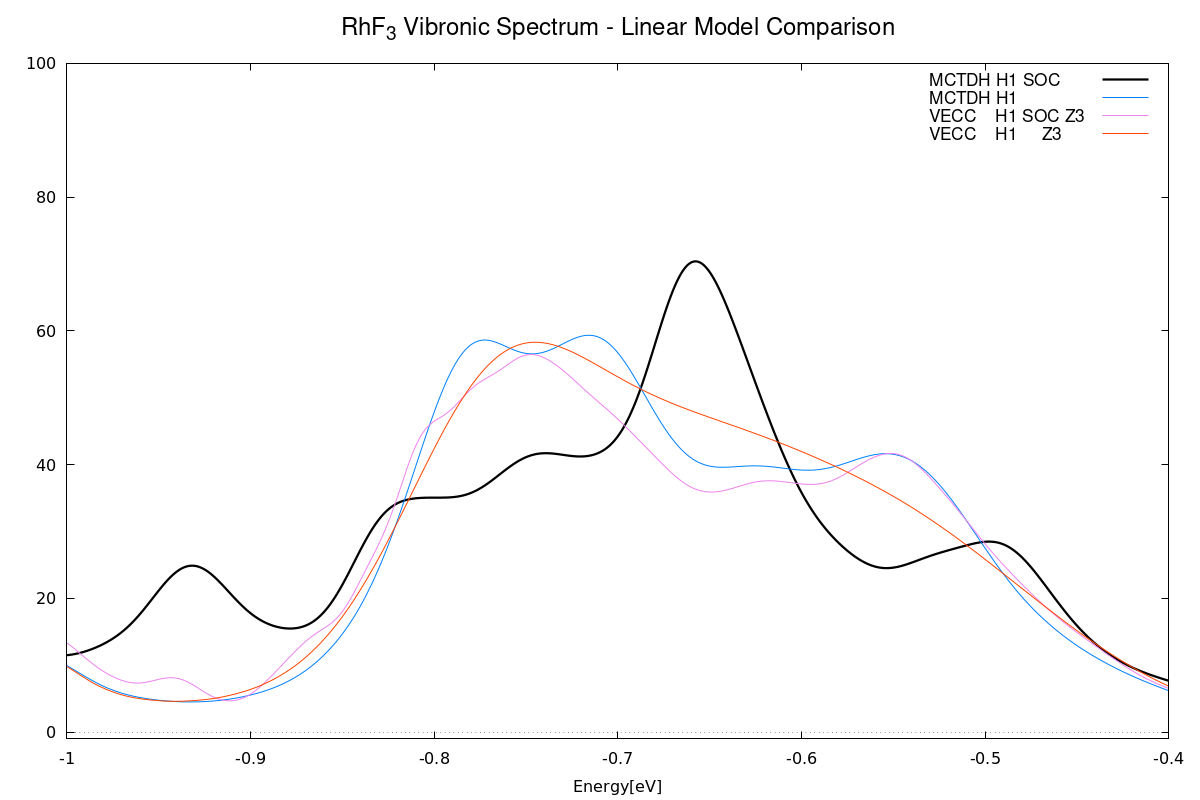
\includegraphics[width=1\columnwidth]{images/RhF3_FINAL/Jun_24_RhF3_Linears.png}
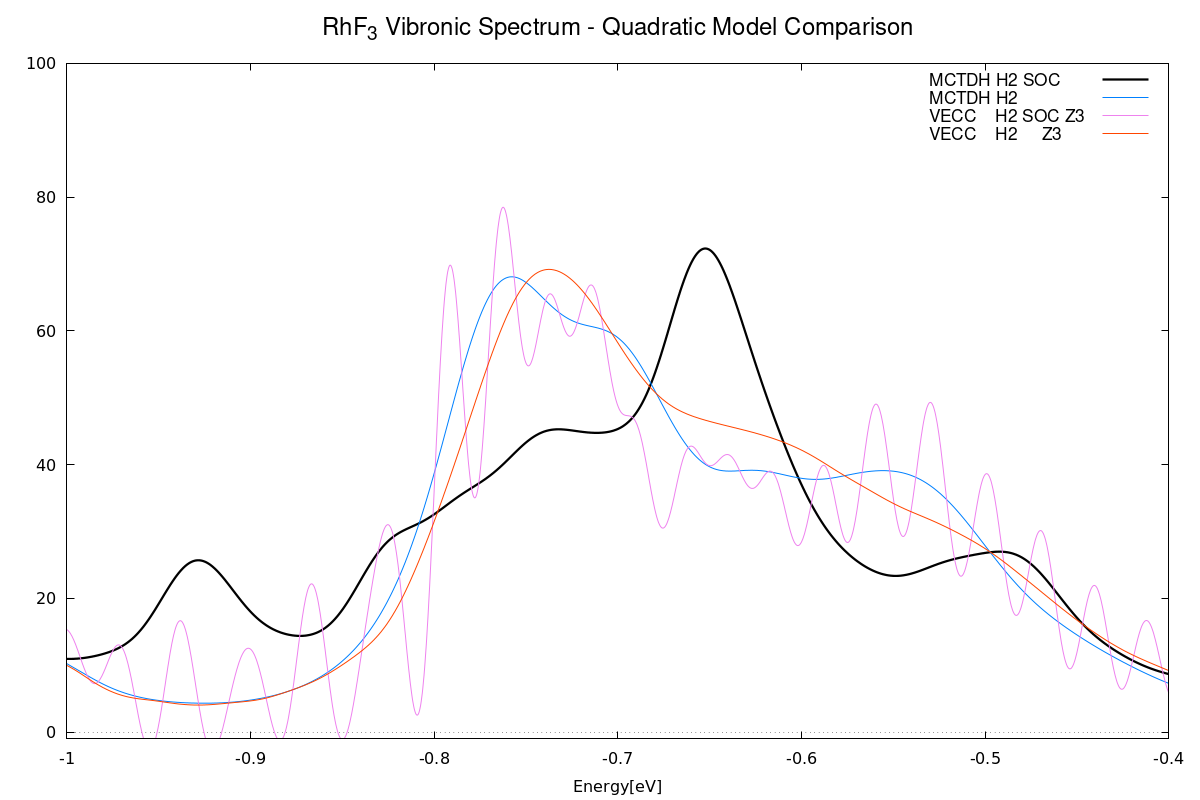
\includegraphics[width=1\columnwidth]{images/RhF3_FINAL/Jun_24_RhF3_Quadratics.png}
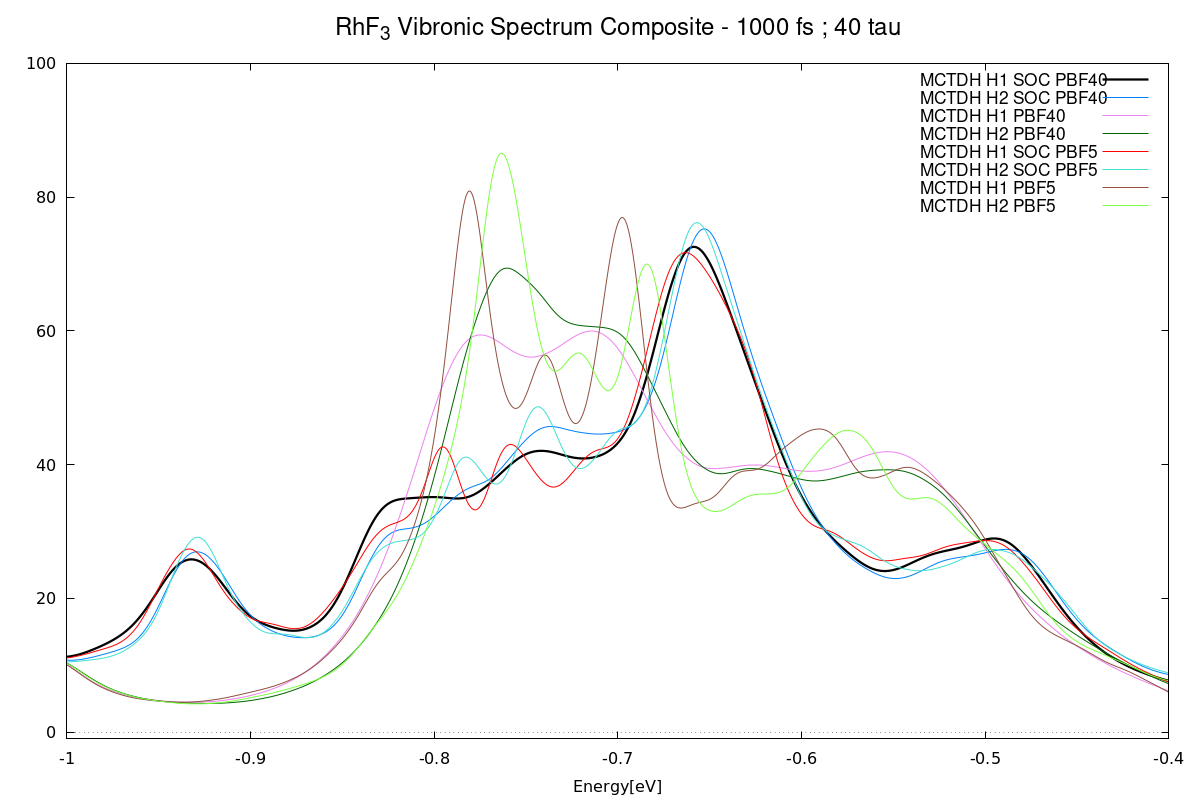
\includegraphics[width=1\columnwidth]{images/RhF3_FINAL/Jun_24_RhF3_longprop_40tau.png}
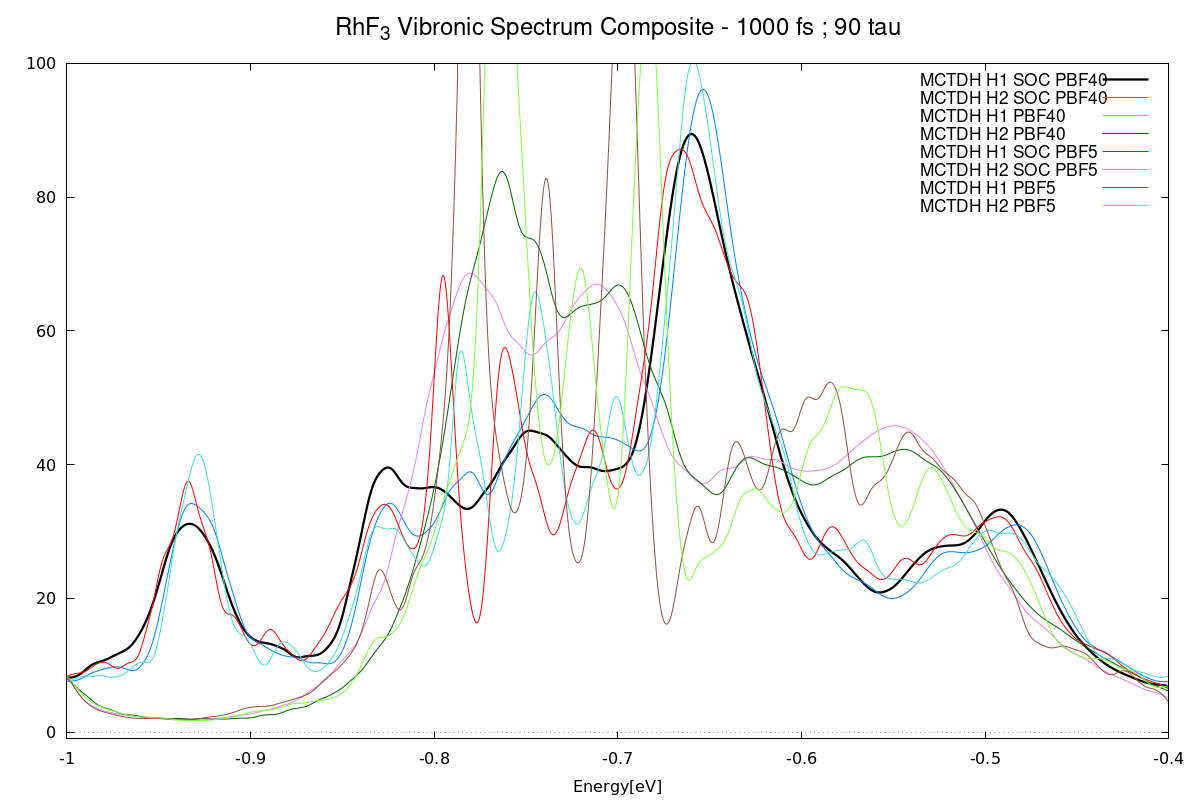
\includegraphics[width=1\columnwidth]{images/RhF3_FINAL/Jun_24_RhF3_longprop_90tau.png}
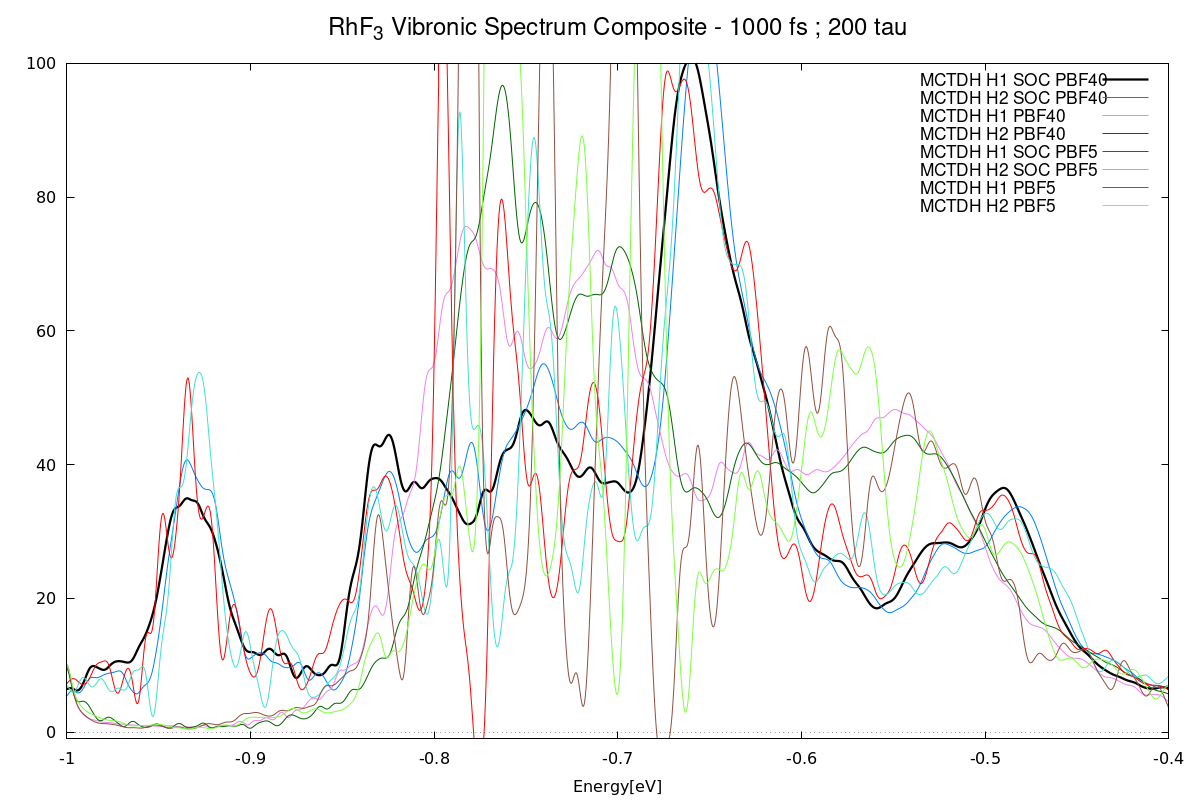
\includegraphics[width=1\columnwidth]{images/RhF3_FINAL/Jun_24_RhF3_longprop_200tau.png}

TAU MAKES A HUGE DIFFERENCE FOR RHF3! ESPECIALLY IF IT IS LONG PROPAGATION MCTDH.\\
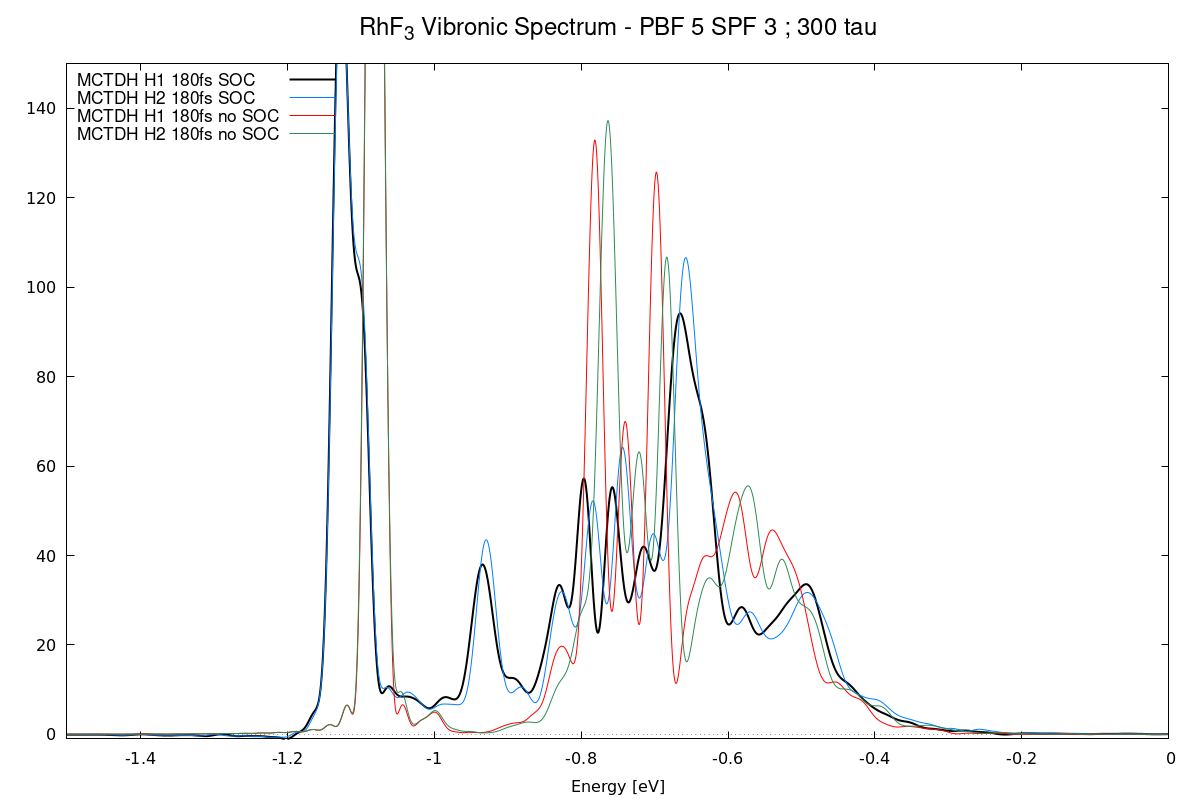
\includegraphics[width=1\columnwidth]{images/Jun_20_RhF3_vanilla_300tau.png} \\

HOWEVER THE PROBLEM IS THAT VECC CANNOT HANDLE LARGE TAU AND CANNOT HANDLE LARGE FS PROPAGATION ELSE DIVERGES SO 180FS 40 TAU IS IDEAL FOR COMPARISON!!

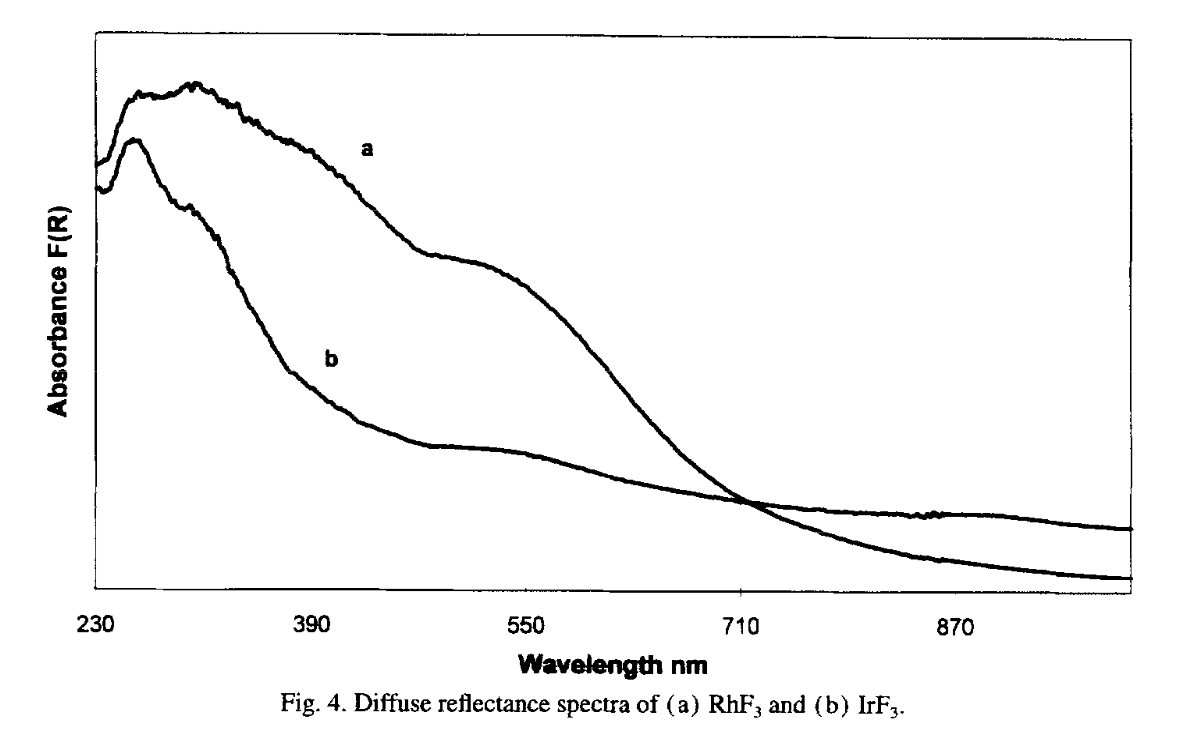
\includegraphics[width=1\columnwidth]{images/COMPARE_EXPERIMENTAL/RhF3_reflectance_hector.PNG}
taken from "UV-visible spectroscopic studies of group 8-10 metal trifluorides" //


add short description of file
show table with Hamiltonian parameters
show image of molecule? (progbably unnnecessary)
show spectra from MCTDH and VECC (maybe show constant, linear, quadratic, SOC?)
discuss the results? are they identical, good this system was just top test xyz, and it behaved as we expected.

% ------------------------------------------------------------------------------------
\subsection{Fe(CO)5}
add short description of file
show table with Hamiltonian parameters
show image of molecule? (progbably unnnecessary)
show spectra from MCTDH and VECC (maybe show constant, linear, quadratic, SOC?)
discuss the results? are they identical, good this system was just top test xyz, and it behaved as we expected.

\begin{figure}[!ht]
    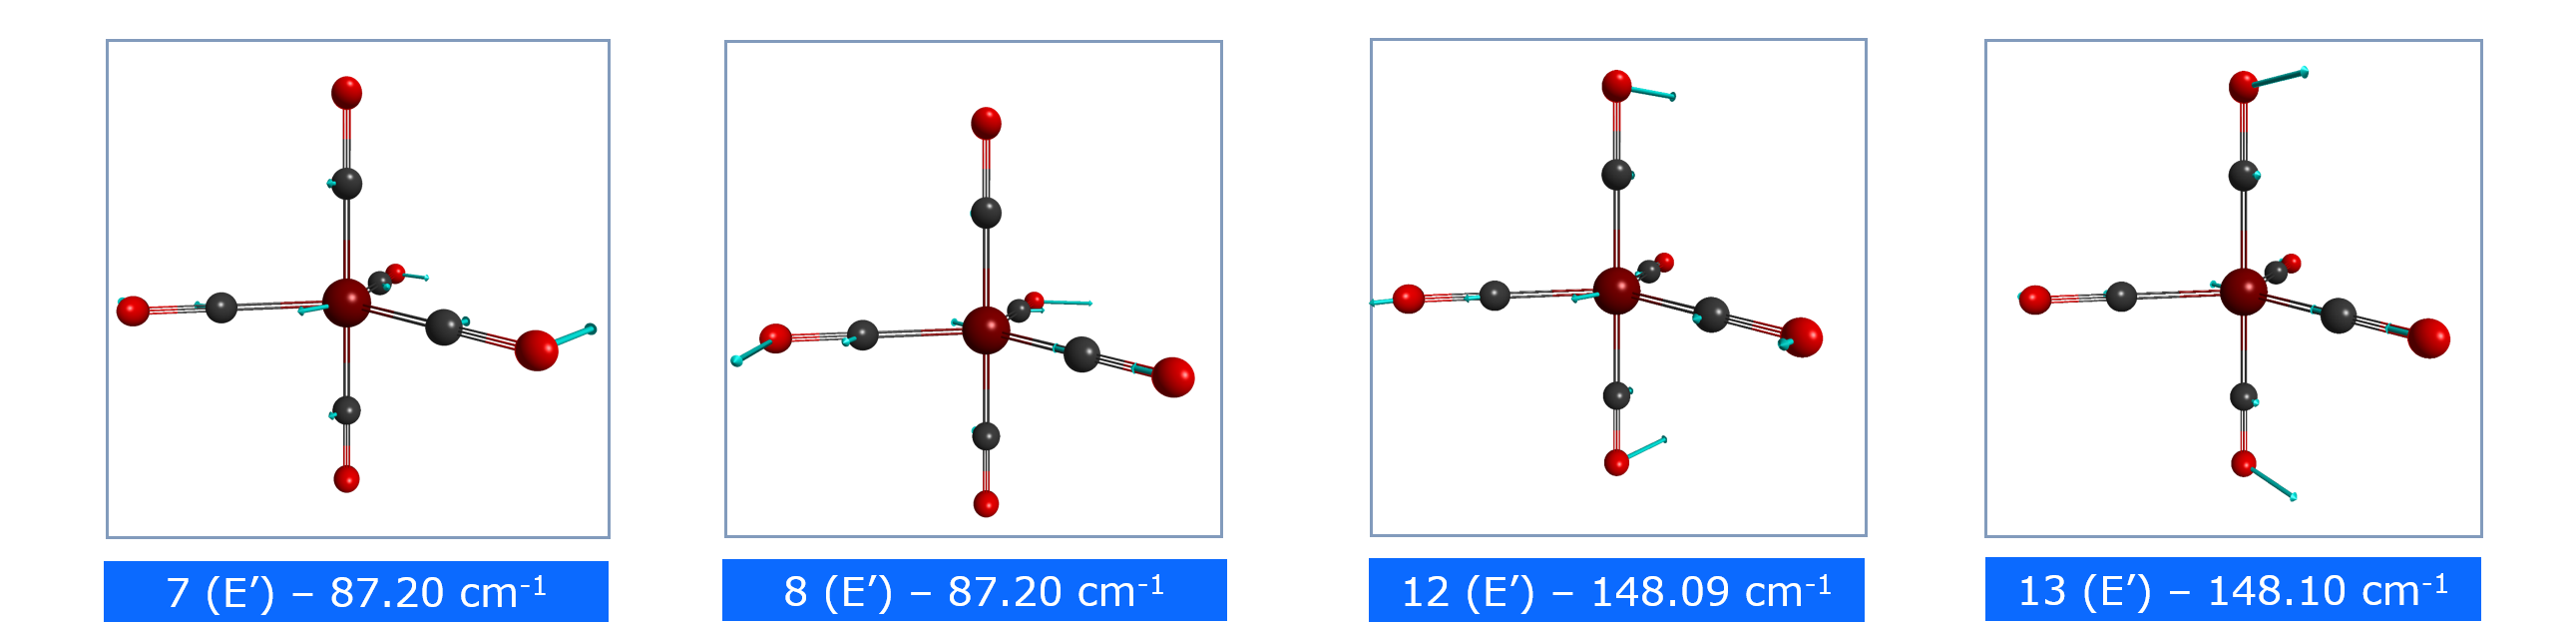
\includegraphics[width=1\columnwidth]{images/screened_former4.png}
    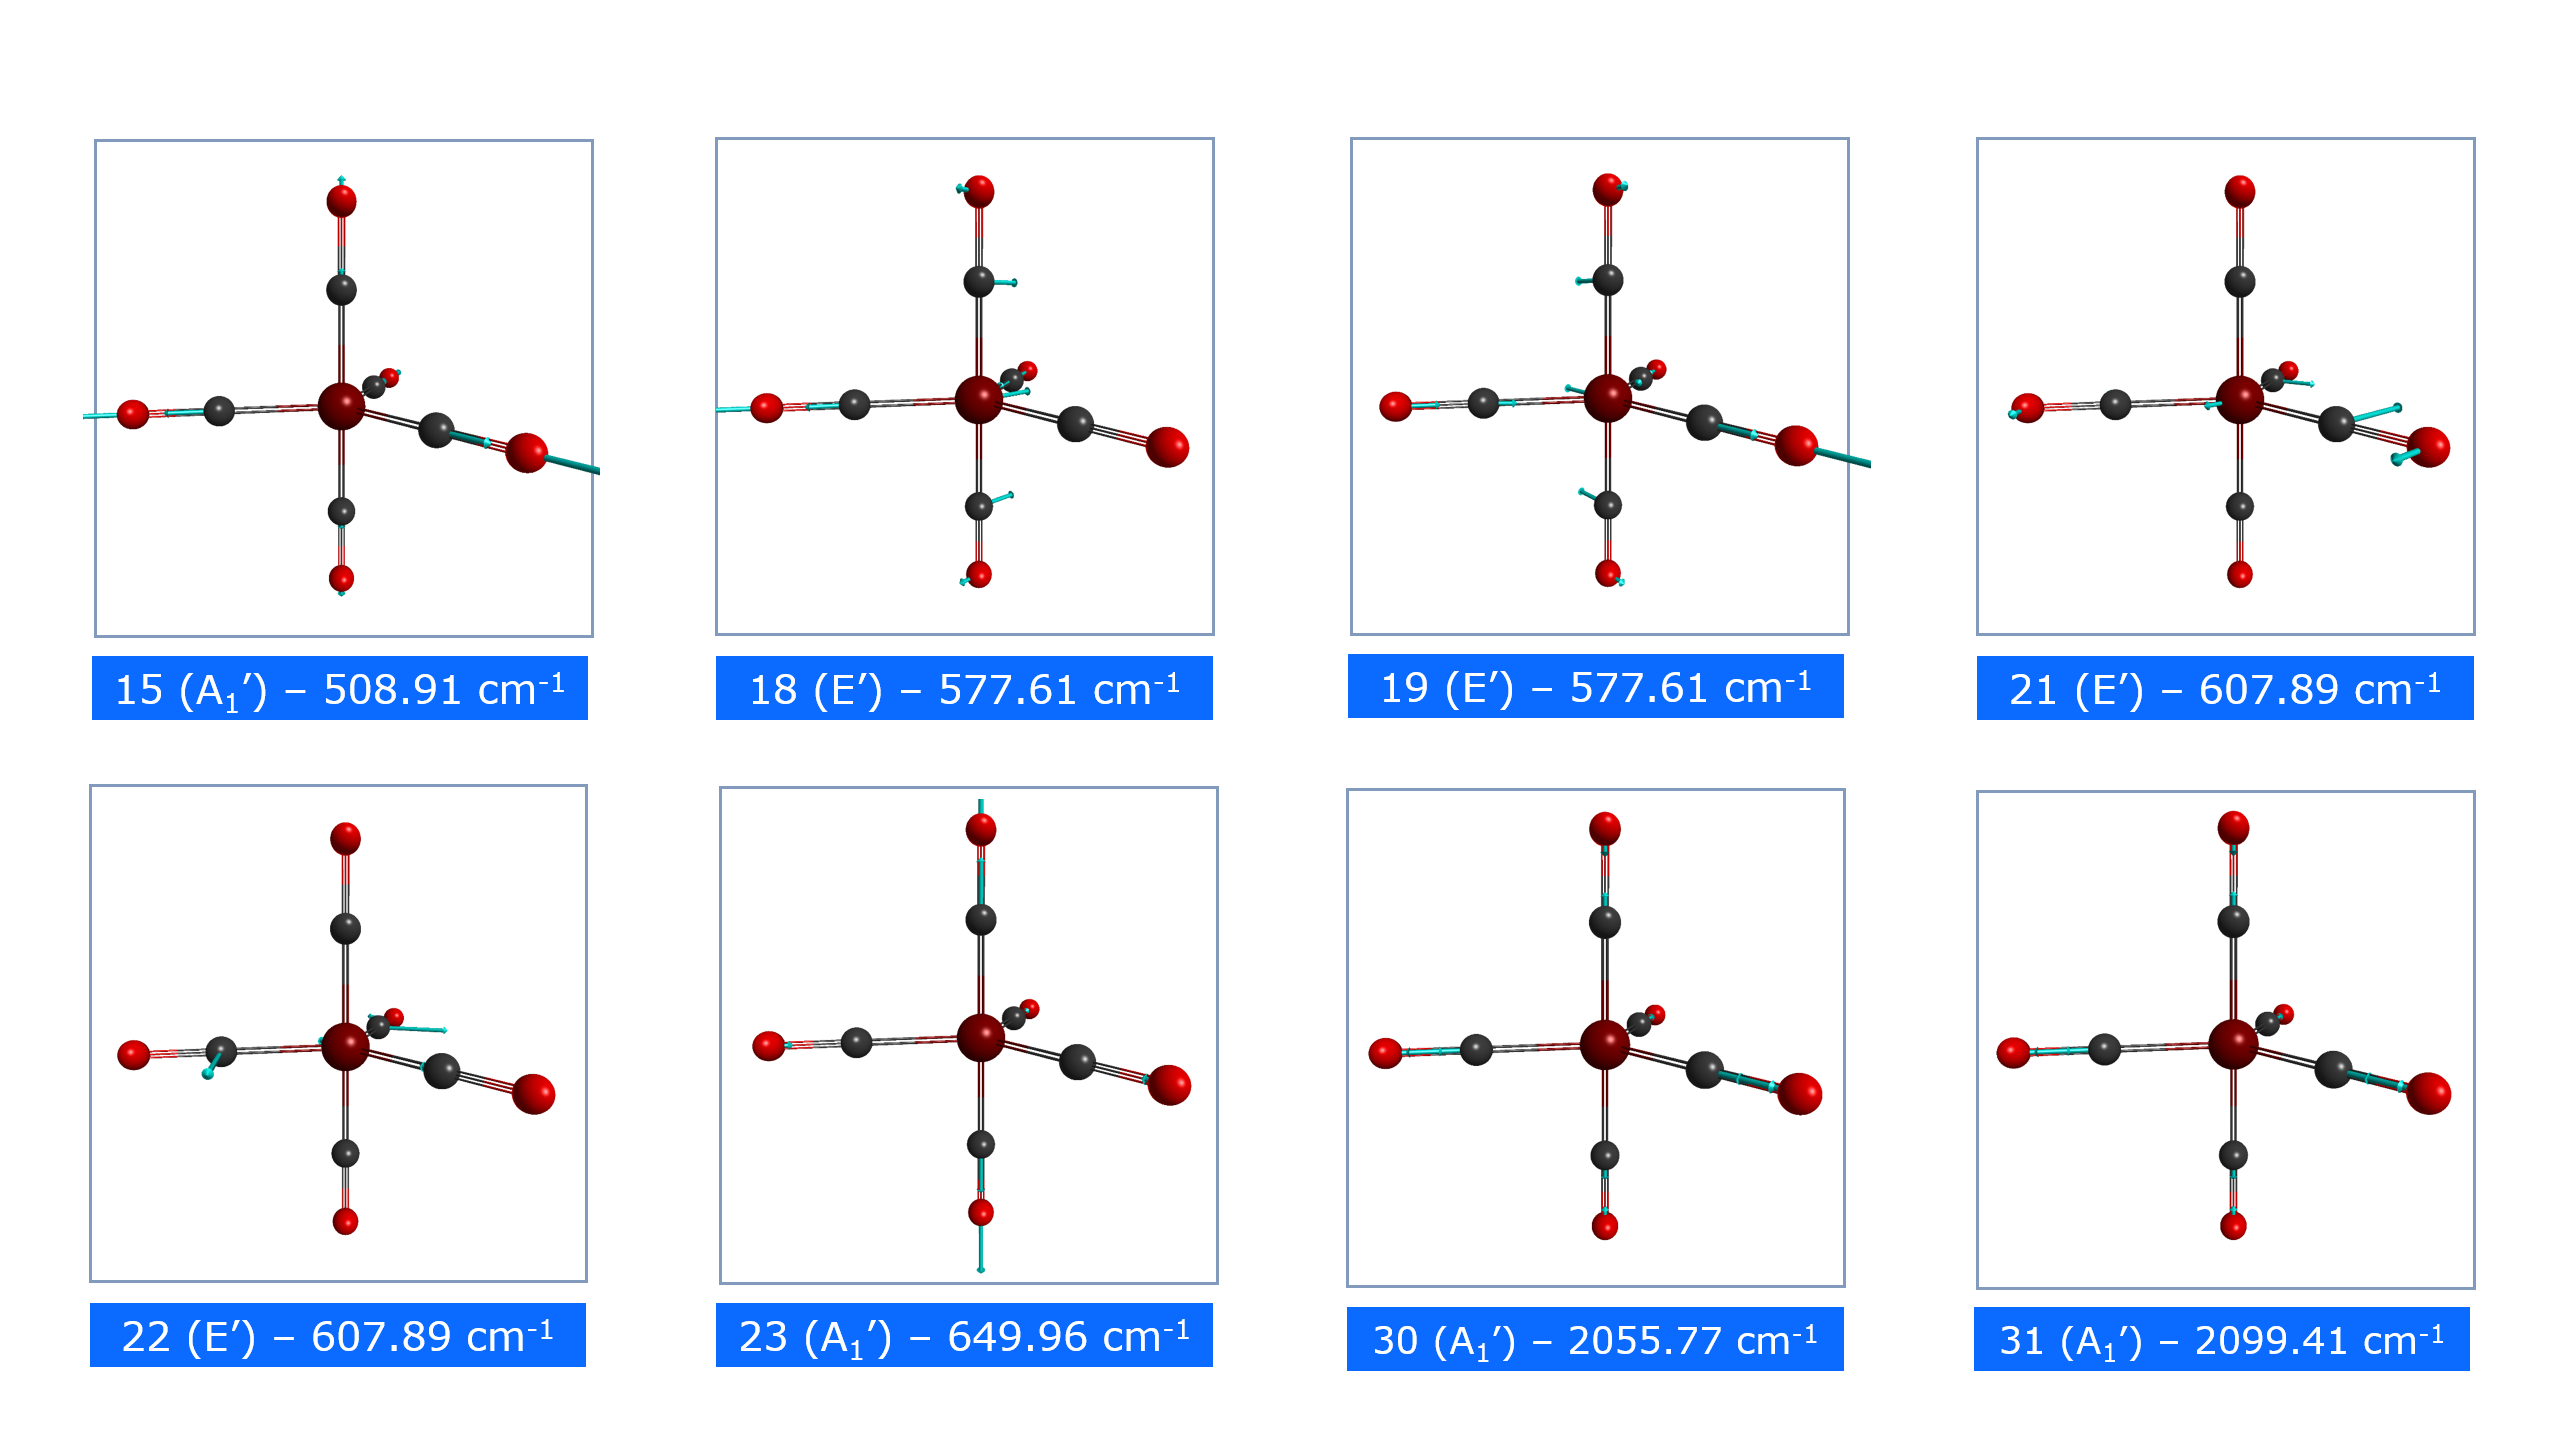
\includegraphics[width=1\columnwidth, trim={0in 0in 0in 0.75in},clip]{images/screened_latter8.png}
    \center
    \small{Fig . Screened 12 out of 27 modes. }
\end{figure}

    

% ------------------------------------------------------------------------------------
\subsection{Vibronic spectra of test case pnictogen hydrides}

% ------------------------------------------------------------------------------------
\subsection{Spectra of \ce{D_{3h}} SOC transition metal complexes (\ce{CoF3} and \ce{RhF3})}

% \section{Dimanganese decacarbonyl, \ce{Mn2(CO)10}}
% https://www.sciencedirect.com/science/article/pii/S0022328X12006237

% ------------------------------------------------------------------------------------
% ------------------------------------------------------------------------------------
\section{Iron pentacarbonyl, \ce{Fe(CO)5}}
% ------------------------------------------------------------------------------------
carbonyl ligand, due to carbonyls' known stabilizing effect on metals

    Using \ce{Fe(CO)5} as an example: we first recognized that the full valence active space was 11o18e. However, doing a oneshot for even the ground state equilibrium geometry calculation did not result in anywhere near convergence. Instead, we had to slowly build up the transition metal compound's ground state geometry by filling in bunches of electrons and orbitals at a time. The initial calculation was a 4+ cation, with a multiplicity of 1. Next, a calculation of 1+ charge and multiplicity of 4, due to three unpaired electrons between a set of a" and e' of orbitals 46 through 48. This calculation resolved the orbital ranking: a" was lower than e'. Finally, a third calculation was ultimately performed on the fully electron-filled molecule and this neutral model yielded the full equilibrium geometry. CHEMICAL INTUITION NEEDED!
    
    We first started by doing an optimization of \ce{Fe(CO)5^4+}. Then, we introduced 2 electrons (multiplicity of 3), and then made it neutral. Observed that the irreducible representation orbital ranking of HOMO was $e'$ and LUMO was $a_{1}'$ After obtaining the equilibrium geometry, we proceeded to fill the active space. 4o4e, 5o8e, 6o8e, 6o10e, 8o10e, 9o12e, and the finally the full valent 11o18e. However, 11o18e did not seem to converge no matter what we tried. So we opted for 8o10e to tide us over and achieve a reasonable spectrum.

    Curse of dimensionality when doing 33 modes ... gigantic ... ML-MCTDH is needed according to Prateek: https://mattermodeling.stackexchange.com/questions/535/what-is-the-largest-system-for-which-vibrationally-resolved-electronic-spectra-h \\

    So we screened modes using effective vibronic coupling magnitude above a threshold. Linear couplings only. See JCTC singlet and triplet fission paper. Heart-wrenching that MCTDH could only compile up to 220k parameters when we needed 260k for our full model. Emailed Prateek and H.D.-Meyer. We can assert that only these 12 modes belong to the model. Incredible struggle, but nah, we'd win. Selected screen modes: [7, 8, 12, 13, 15, 18, 19, 21, 22, 23, 30, 31]. 12 out of 27. TZ: show a spreadsheet of screenshots here, displaying the ones we selected, does it make sense according to out analysis? \\

    (see email with Dieter) We have good news. Prof. Meyer advised that the MCTDH-84 version I was running was outdated and that upgrading to the newest 86 version would do the trick. Fortunately Toby had a copy of 86 too on hand. Not only has the parameter limitation seemed to be resolved, but it similarly resolves a secondary issue in 84 where parallelized runs where erroring out (but works now in 86!).

    Stitching together various functionalities, tuning

    May 29th: we have done plotting of diabatic energies today and saw that mode 15 was equatorial dissociation and mode 23 was axial dissociation. Equatorial dissociation leads to one of the COs on the horizontal plane leaving, resulting in the axial COs to bend down and resulting in Td symmetry. Whereas, axial dissociation results in one CO on principal axis leaving and resulting in C3v symmetry.

    An optimal and desirable system for exhibiting both JT and SOC effects is a large iron complex with low-lying degenerate electronic states and carbonyl ligand, due to carbonyls' known stabilizing effect on metals (Nooijen discussion referenece)

    \url{https://stackoverflow.com/questions/19412382/gnuplot-line-types#19420678}

    We are using ORMAS+GMCPT!
    \url{https://ccl.scc.kyushu-u.ac.jp/~nakano/gmcpt.html}

    Normally we use Douglas-Kroll (DK) in the $\$relfwn$ group, howeveer Sapporo basis sets like RELWFN=LUT-IOTC instead.
    
    Scale breaks things. We have to fix things, redesign, change this, change that... \\
    Emphasize the technical hiccups, airplane dashboard ... It is fickle. On a macro level VECC gets it right, however does not get the fine structure peaks. 

We cannot simplify everything down to a one-size fits all simple model. The sheer amount of parameters and caveats each spectra run takes translates into it being incomplete in some way if we do not alter the parameters specific for the case we are looking at. Overall you have to make decisions and cleverly choose an array of compatible parameters. Having reservations about a job is needed, oftentimes a double or even triple check is prudent.


FeCO SOC effect not observed probably because it is too subtle and weak. 

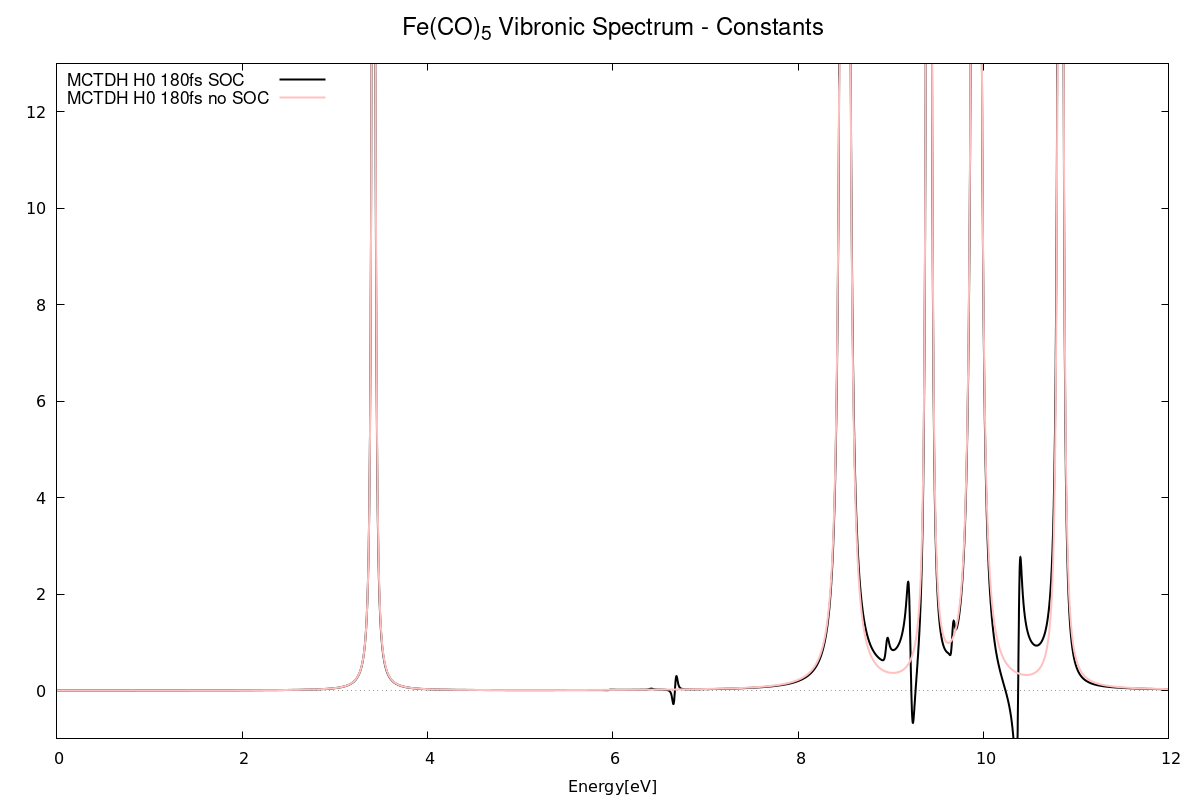
\includegraphics[width=1\columnwidth]{images/Jun_17_FeCO_constants.png}

\includegraphics[width=1\columnwidth]{images/op_FeCO3Q_17st_PBF7_tf100.00_xyz_spectrum_1900by900.png}

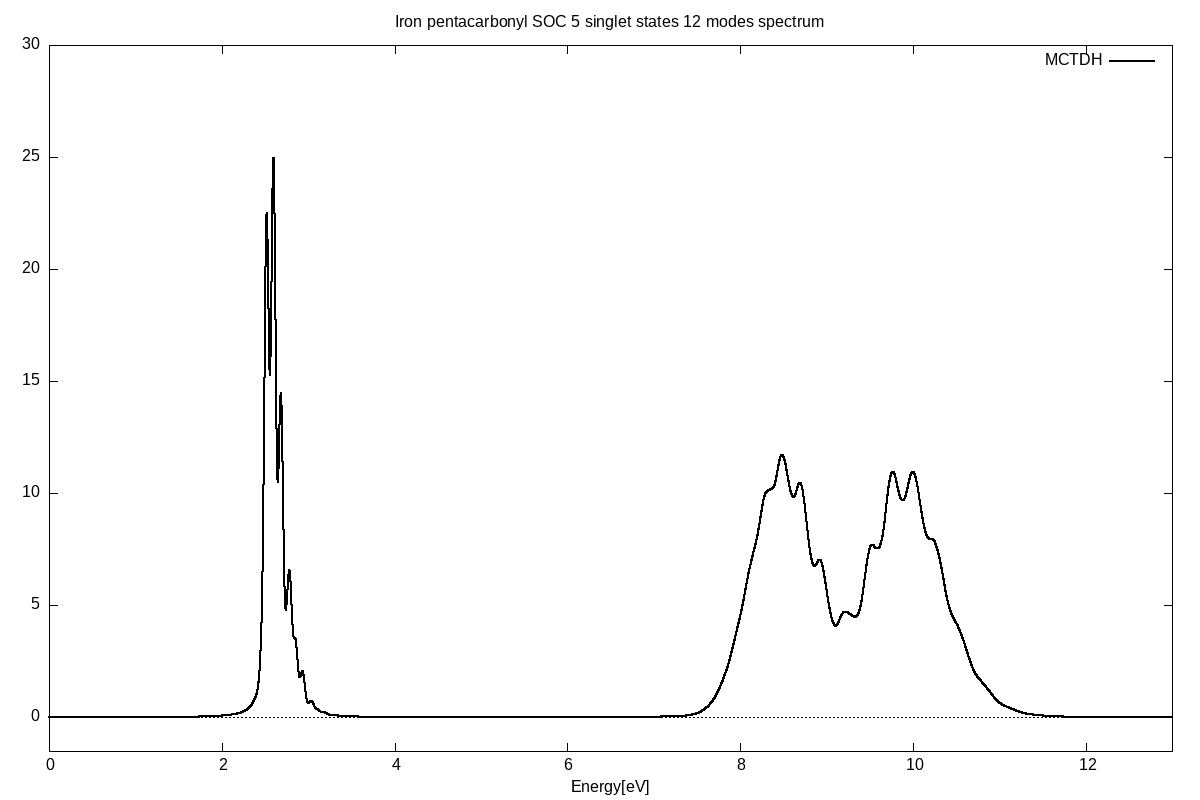
\includegraphics[width=1\columnwidth]{images/op_FeCO3Q_5st_PBF7_tf100.00_xyz_spectrum_5singlets.png}

\includegraphics[width=1\columnwidth]{images/Jun_18_FeCO_waterfall_composite_collated.png}

\includegraphics[width=1\columnwidth]{images/Jun_18_FeCO_vanilla_vs_orig.png}

\includegraphics[width=1\columnwidth]{images/FeCO_FINAL/Jun_25_FeCO_waterfall_composite_collated.png}
\includegraphics[width=1\columnwidth]{images/FeCO_FINAL/Jun_25_FeCO_MCTDH_SOC.png}
\includegraphics[width=1\columnwidth]{images/FeCO_FINAL/Jun_25_FeCO_VECC_SOC.png}
\includegraphics[width=1\columnwidth]{images/FeCO_FINAL/Jun_25_FeCO_higherpeak_collated.png}




\includegraphics[width=1\columnwidth]{images/COMPARE_EXPERIMENTAL/FeCO_atkins.PNG}
taken from "High-resolution X-ray absorption spectroscopy of iron carbonyl complexes" //

\includegraphics[width=1\columnwidth]{images/COMPARE_EXPERIMENTAL/FeCO_odwyer.PNG}
taken from "Infrared Spectra and Normal Coordinate Analysis of Iron Pentacarbonyl” // 



\includegraphics[width=1\columnwidth]{images/pes_progression.PNG}


\ce{D_{3h}} Character Table
\begin{table}[h]\centering
    \caption{Character Table for the $D_{3h}$ Point Group}
    \begin{tabular}{c|cccccc}
        \hline
        $D_{3h}$ & $E$ & $2C_3$ & $3C'_2$ & $\sigma_h$ & $2S_3$ & $3\sigma_v$ \\
        \hline
        $A'_1$   & 1 &  1 &  1 &  1 &  1 &  1 \\
        $A'_2$   & 1 &  1 & -1 &  1 &  1 & -1 \\
        $A''_1$  & 1 &  1 &  1 & -1 & -1 & -1 \\
        $A''_2$  & 1 &  1 & -1 & -1 & -1 &  1 \\
        $E'$     & 2 & -1 &  0 &  2 & -1 &  0 \\
        $E''$    & 2 & -1 &  0 & -2 &  1 &  0 \\
        \hline
    \end{tabular}
    \label{tab:character_table_d3h}
\end{table}

\clearpage
\begin{lstlisting}[frame=single, language=xml]
 Maximal values (all times and states);  final time:     8.20 fs
   #  dof     grid(begin)    grid(end)      basis(begin)   basis(end)
   1  v01     0.003819209    0.004304504    1.000000000    0.069330648
   2  v02     0.002394854    0.002907799    1.000000000    0.094262965
   3  v03     0.006564292    0.011120993    1.000000000    0.054929234
   4  v04     0.008430379    0.007697208    1.000000000    0.060806006
   5  v05     0.000016531    0.378852129    1.000000000    0.008608200
   6  v06     0.000240223    0.018687338    1.000000000    0.000193951
   7  v07     0.000044060    0.046103045    1.000000000    0.000832838
   8  v08     0.030122789    0.021198401    1.000000000    0.007997538
   9  v09     0.053021628    0.015153312    1.000000000    0.010167416
  10  v10     0.000000222    0.360995024    1.000000000    0.029714981
  11  v11     0.001646049    0.000000013    1.000000000    0.000000208
  12  v12     0.000002498    0.001008901    1.000000000    0.000000019
\end{lstlisting}

and lines <x>\texttt{5  v05     0.000016531    0.378852129    1.000000000    0.008608200} and <x> \texttt{ 10  v10     0.000000222    0.360995024    1.000000000    0.029714981}



\begin{lstlisting}[frame=single, language=xml]
rdgpop86 1 0
 mode dof  dim   DVR     modelabel
   1    1    8   HO      v01
   1    2    8   HO      v02
   1    3   10   HO      v03
   1    4   10   HO      v04
   2    5   30   HO      v05
   2    6   20   HO      v06
   2    7   20   HO      v07
   3    8   30   HO      v08
   3    9   30   HO      v09
   3   10   30   HO      v10
   4   11   16   HO      v11
   4   12   12   HO      v12

 Maximal values (all times and states);  final time:     8.20 fs
   #  dof     grid(begin)    grid(end)      basis(begin)   basis(end)
   1  v01     0.003819209    0.004304504    1.000000000    0.069330648
   2  v02     0.002394854    0.002907799    1.000000000    0.094262965
   3  v03     0.006564292    0.011120993    1.000000000    0.054929234
   4  v04     0.008430379    0.007697208    1.000000000    0.060806006
   5  v05     0.000016531    0.378852129    1.000000000    0.008608200 /*bf*/
   6  v06     0.000240223    0.018687338    1.000000000    0.000193951
   7  v07     0.000044060    0.046103045    1.000000000    0.000832838
   8  v08     0.030122789    0.021198401    1.000000000    0.007997538
   9  v09     0.053021628    0.015153312    1.000000000    0.010167416
  10  v10     0.000000222    0.360995024    1.000000000    0.029714981 /*bf*/
  11  v11     0.001646049    0.000000013    1.000000000    0.000000208
  12  v12     0.000002498    0.001008901    1.000000000    0.000000019

**********************************************************

rdcheck86 0 0

mode: No. of SPFs per state : modelabels
   1 :   6  10  10   8  12   1 :  v01 v02 v03 v04
   2 :   6   8   8   8   8   1 :  v05 v06 v07
   3 :   6  10  10  10  12   1 :  v08 v09 v10
   4 :   5   5   5   5   5   1 :  v11 v12

 tinit =      0.000 fs,    tout =      0.100 fs
----------------------------------------------------------
 Maximum over time of lowest nat.-weight;    time :      50.00 fs
 mode    s = 1      s = 2      s = 3      s = 4      s = 5      s = 6
   1   2.848E-03  7.210E-03  6.974E-03  9.912E-03  4.711E-03  0.000E+00
   2   2.567E-03  6.879E-03  7.224E-03  8.111E-03  8.778E-03  0.000E+00
   3   2.259E-03  9.978E-03  9.306E-03  6.689E-03  8.065E-03  0.000E+00
   4   8.478E-05  3.963E-06  6.035E-06  1.653E-05  4.295E-05  0.000E+00

\end{lstlisting}

\begin{lstlisting}[frame=single, language=xml,]
#         Electronic transition moments         #
# --------------------------------------------- #

Ex_s00_s01               =    0.100000000   , au
Ex_s01_s02               =    0.100000000   , au
Ex_s00_s02               =    0.100000000   , au
Ex_s01_s03               =    0.100000000   , au
Ex_s02_s03               =    0.100000000   , au
Ex_s00_s03               =    0.100000000   , au


#         Electronic transition moments         #
# --------------------------------------------- #

Ex_s00_s01               =    0.000000000    , au
Ex_s01_s02               =    0.000000000    , au
Ex_s00_s02               =   -0.097354000    , au
Ex_s01_s03               =   -0.000000000    , au
Ex_s02_s03               =    0.000000000    , au
Ex_s00_s03               =   -0.097353000    , au
\end{lstlisting}


No matter how much we tried to increase the primitive basis grid size, the end state is always highly populated, meaning that the potentials are unbound.



% \section{Tris(bipyridine)ruthenium(II) chloride, \ce{[Ru(bpy)3]Cl2}}
%     \subsection{https://en.wikipedia.org/wiki/Tris(bipyridine)ruthenium(II)_chloride}
    
% \section{https://pubs.acs.org/doi/10.1021/ic800091y}

% \section{Copper halides}

\newpage
AVOID DOING TDH AT ALL COSTS!!! IT EXPLODED MY SCRATCH
\begin{lstlisting}
[bjb2chen@narval3 ~]$ diskusage_report
                             Description                Space           # of files
                /home (project bjb2chen)             636M/50G             12k/500k
             /scratch (project bjb2chen)              19T/20T            18k/1000k
         /project (project def-mnooijen)           138G/1000G             14k/500k
        /nearline (project def-mnooijen)            98k/1000G               4/5000

    [bjb2chen@narval3 Apr26_redo_SOC]$ du -ah SOC_CORRECTION/ | sort -hr | head -n 20
19T     SOC_CORRECTION/TDH/mctdh/op_FeCO27Q_17st_fullmodes

\end{lstlisting}

\newpage

Haruyuki Nakano. Hisao Nakamura. See conversation with Neil on June 3rd.

SOC: https://pubs.aip.org/aip/jcp/article/146/14/144103/195065 Metal trifluorides: https://www.scie
Diabatic states: G. J. Atchity and K. Ruedenberg, Theor. Chem. Acc. 97, 47 (1997).https://doi.org/10.
https://pubs.aip.org/aip/jcp/article/115/22/10353/946057/The-direct-calculation-of-diabatic-
states-based-on
UV spectra: https://onlinelibrary.wiley.com/doi/10.1002/qua.10724
Linear vibronic models: https://pubs.acs.org/doi/10.1021/acs.jctc.1c00022 (Santoro)

We are using ORMAS+GMCPT! Student guide that really crystallized my knowledge of GMC-QDPT:
\url{ttps://ccl.scc.kyushu-u.ac.jp/~nakano/gmcpt.html}

% file:///Users/bjc/Downloads/configurational_uniformity_hisao.pdf - configurational uniformity paper

% J Comput Chem 23: 1166–1175, 2002 : GMC-QDPT paper
    
% \subsection{https://pubs.acs.org/doi/10.1021/jacs.2c01469} - this is the iron pentacarbonyl modern paper
% \subsection{https://pubs.acs.org/doi/10.1021/jp992474u}
% \subsection{https://pubs.aip.org/aip/jcp/article/75/6/2560/791508/The-Jahn-Teller-effect-in-the-photoelectron} \\

Iron pentacarbonyl, haruyuki nakano and mark s gordon https://pubs.rsc.org/en/content/articlepdf/1999/cp/a808518h


This is a very good diagram showing interdependencies: https://en.wikipedia.org/wiki/Complete\_active\_space\_perturbation\_theory

This is a good consideration for future work, running the calculations via GPU acceleration: 
https://www.nvidia.com/es-la/data-center/gpu-accelerated-applications/gamess/

MCTDH troubleshooting
% https://www.pci.uni-heidelberg.de/tc/usr/mctdh/doc.86/mctdh/trouble.html#redim 

% GAMESS input documentation: https://www.msg.chem.iastate.edu/gamess/GAMESS_Manual/docs-input.txt


\url{https://en.wikipedia.org/wiki/Dung_beetle}


\lstset{
  basicstyle=\ttfamily\footnotesize,
  keywordstyle=\color{blue}\bfseries,
  stringstyle=\color{red},
  commentstyle=\color{green}\itshape,
  numbers=left,
  numberstyle=\tiny\color{gray},
  stepnumber=1,
  numbersep=5pt,
  frame=single,
  breaklines=true,
  captionpos=b,
  escapeinside={(*@}{@*)},
  morekeywords={def, print} % Custom keywords
}

\begin{lstlisting}[language=Python, caption=Example Python Code]
# This is a comment
def hello_world():
    print("Hello, world!")
\end{lstlisting}

\input{chapters/caveats}

\chapter{Conclusion}
Diabatization is at the heart of current vibronics research. Although it provides a numerical result, it can be applied to generalized situations. Perhaps one day there will be analytical models that can solve vibronics entirely.


\url{https://www.sci.uwaterloo.ca/~nooijen/website/research.html}
\url{https://yorkspace.library.yorku.ca/server/api/core/bitstreams/302f290d-535e-462e-8ca5-1e59fc3b376f/content}
\url{https://pubs.acs.org/doi/10.1021/jp0456990}
\url{https://www.sci.uwaterloo.ca/~nooijen/website/vibron/VC/Manual.pdf}%



%======================================================================
%----------------------------------------------------------------------
% END MATERIAL
% Bibliography, Appendices, Index, etc.
%----------------------------------------------------------------------
\ifendmatter%
% Bibliography


% This specifies the location of the file containing the bibliographic information.
% It assumes you're using BibTeX to manage your references (if not, why not?).
\ifprintversion%
    \cleardoublepage% This is needed if the "book" document class is used, to place the anchor in the correct page, because the bibliography will start on its own page.
\else%
    \clearpage% % Use \clearpage instead if the document class uses the "oneside" argument
\fi

\phantomsection% % With hyperref package, enables hyperlinking from the table of contents to bibliography

% The following statement causes the title "References" to be used for the bibliography section:
% \renewcommand*{\bibname}{References}

% Add the References to the Table of Contents
\addcontentsline{toc}{chapter}{\textbf{Bibliography}}

%\renewcommand*{\bibfont}{\scriptsize}

% The following statement causes the specified references to be added to the bibliography even if they were not cited in the text.
% The asterisk is a wildcard that causes all entries in the bibliographic database to be included (optional).
\nocite{*}
\printbibliography[title={Bibliography}]

%----------------------------------------------------------------------

Appendices (commented out for now)

% The \appendix statement indicates the beginning of the appendices.
\ifprintversion%
    \cleardoublepage\phantomsection%
\else
    \thispagestyle{plain}
    \pagestyle{plain}
    \clearpage
\fi
%
\appendix
\appendixpage%

% Add an un-numbered title page before the appendices and a line in the Table of Contents
% \chapter*{APPENDICES}
% \addcontentsline{toc}{chapter}{APPENDICES}

% Appendices are just more chapters, with different labeling (letters instead of numbers).
%----------------------------------------------------------------------
%----------------------------------------------------------------------
\chapter{Name of first appendix chapter\label{app:pimc_notes_chapter}}
%----------------------------------------------------------------------

% \input{base_latex_files/appendices/lst_smatrix_elements}


% GLOSSARIES (Lists of definitions, abbreviations, symbols, etc. provided by the glossaries-extra package)
% -----------------------\------
% \iffinalize \addcontentsline{toc}{chapter}{Glossary} \chapter*{Glossary} \clearpage \else \fi
% \printglossaries   % this prints the acronyms
\clearpage%
\phantomsection%     % allows hyperref to link to the correct page
\fi  % NEEDED TO END THE `ifendmatter` ABOVE
% \iffinalize \addcontentsline{toc}{chapter}{Index} \chapter*{Index} \clearpage \else \fi
%----------------------------------------------------------------------


%----------------------------------------------------------------------
% rememeber to run "makeglossaries benny_chen" from terminal in the project folder
%----------------------------------------------------------------------
\end{document} % end of logical document
%----------------------------------------------------------------------

% all acronyms should be written out in full the first time used
% seperately in the abstract and in the main text



